\chapter{Introduction}
Loudspeakers today come in all sizes, types and shapes, has existed for over a century and is used by all, but it has yet to be perfected. In the 1980's an entirely new loudspeaker type, the active loudspeaker, began popping up and has gained popularity ever since. The rise of the active loudspeaker can probably be attributed to the rise of the digital signal processing which means that there are endlessly possibilities of processing a input signal like equalizing, compressing or synthesizing for example.

These possibilities means the the potential of the active loudspeaker is far greater than the passive loudspeaker because the active loudspeaker has the amplifier   

Danger

protection

Optimal sound 

% The market for Bluetooth loudspeakers has been growing considerably the last few years. According to \gls{CTA} the revenue of Bluetooth loudspeakers has been growing 69 \% between 2013 and 2014 \cite{sou:CTA}. The high growth is partly due to the increasing usage of smartphones and music streaming services, such as Spotify. As a result it is now more desirable for some users to wirelessly connect the smartphone to an audio system through for instance Bluetooth. By doing so, the user can use the smartphone to remote control his or her audio system. 

% Wireless loudspeakers are primarily active loudspeakers and are usually small. As a result of the physical limitations the loudspeaker may not play very loud and the performance of the loudspeaker in the bass region is limited.   

%To compensate for the lack of bass the user may want to boost the bass in order to achieve a more rich sound. However because of the limited size, increasing the bass can potentially lead to sound distortions caused by clipping or enclosure vibrations. The measurements in \autoref{fig:introduction} shows how a boost in the bass region can distort the sound.

% \begin{figure}[H]
% \centering
% \tikzsetnextfilename{signal}
% % This file was created by matlab2tikz.
%
%The latest updates can be retrieved from
%  http://www.mathworks.com/matlabcentral/fileexchange/22022-matlab2tikz-matlab2tikz
%where you can also make suggestions and rate matlab2tikz.
%
\definecolor{mycolor1}{rgb}{0.00000,0.44700,0.74100}%
\definecolor{mycolor2}{rgb}{0.85000,0.32500,0.09800}%
%
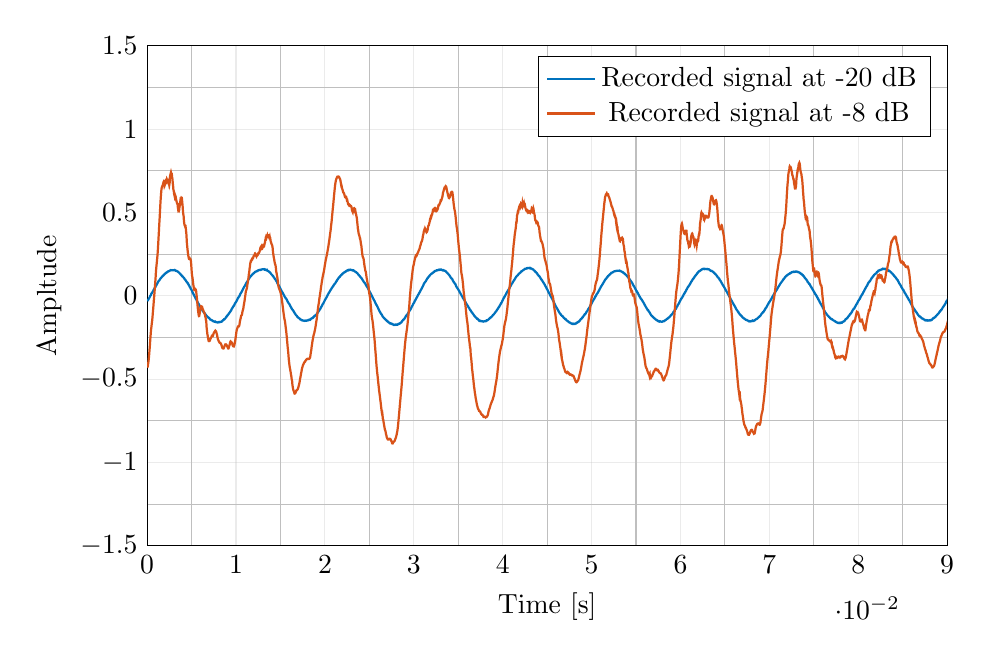
\begin{tikzpicture}

\begin{axis}[%
width=4in,
height=2.5in,
    grid = both,
    minor tick num=1,
    every major grid/.style={opacity=0.3},
    major tick length=0pt,
    minor tick length=0pt,
scale only axis,
xmin=0,
xmax=0.09,
xlabel={Time [s]},
ymin=-1.5,
ymax=1.5,
ylabel={Ampltude},
axis background/.style={fill=white}
]
\addplot [color=mycolor1,solid,thick]
  table[row sep=crcr]{%
2.26757369614512e-05	-0.0328369140625\\
4.53514739229025e-05	-0.02972412109375\\
6.80272108843537e-05	-0.027435302734375\\
9.0702947845805e-05	-0.024932861328125\\
0.000113378684807256	-0.023895263671875\\
0.000136054421768707	-0.02191162109375\\
0.000158730158730159	-0.01983642578125\\
0.00018140589569161	-0.018402099609375\\
0.000204081632653061	-0.01605224609375\\
0.000226757369614512	-0.014068603515625\\
0.000249433106575964	-0.011749267578125\\
0.000272108843537415	-0.009124755859375\\
0.000294784580498866	-0.006683349609375\\
0.000317460317460317	-0.00439453125\\
0.000340136054421769	-0.001434326171875\\
0.00036281179138322	0.000579833984375\\
0.000385487528344671	0.001953125\\
0.000408163265306122	0.003631591796875\\
0.000430839002267574	0.007354736328125\\
0.000453514739229025	0.0113525390625\\
0.000476190476190476	0.013397216796875\\
0.000498866213151927	0.01416015625\\
0.000521541950113379	0.0147705078125\\
0.00054421768707483	0.0172119140625\\
0.000566893424036281	0.020050048828125\\
0.000589569160997732	0.021759033203125\\
0.000612244897959184	0.0238037109375\\
0.000634920634920635	0.026397705078125\\
0.000657596371882086	0.027740478515625\\
0.000680272108843537	0.02886962890625\\
0.000702947845804989	0.031829833984375\\
0.00072562358276644	0.03570556640625\\
0.000748299319727891	0.0372314453125\\
0.000770975056689342	0.038848876953125\\
0.000793650793650794	0.041229248046875\\
0.000816326530612245	0.0435791015625\\
0.000839002267573696	0.0457763671875\\
0.000861678004535147	0.047821044921875\\
0.000884353741496599	0.050567626953125\\
0.00090702947845805	0.05145263671875\\
0.000929705215419501	0.052490234375\\
0.000952380952380952	0.0550537109375\\
0.000975056689342404	0.05914306640625\\
0.000997732426303855	0.0614013671875\\
0.00102040816326531	0.062103271484375\\
0.00104308390022676	0.06439208984375\\
0.00106575963718821	0.066558837890625\\
0.00108843537414966	0.068572998046875\\
0.00111111111111111	0.0709228515625\\
0.00113378684807256	0.074066162109375\\
0.00115646258503401	0.076202392578125\\
0.00117913832199546	0.077545166015625\\
0.00120181405895692	0.079559326171875\\
0.00122448979591837	0.0819091796875\\
0.00124716553287982	0.0850830078125\\
0.00126984126984127	0.08746337890625\\
0.00129251700680272	0.08843994140625\\
0.00131519274376417	0.09027099609375\\
0.00133786848072562	0.09173583984375\\
0.00136054421768707	0.0921630859375\\
0.00138321995464853	0.09375\\
0.00140589569160998	0.095672607421875\\
0.00142857142857143	0.097320556640625\\
0.00145124716553288	0.099090576171875\\
0.00147392290249433	0.101531982421875\\
0.00149659863945578	0.104339599609375\\
0.00151927437641723	0.10528564453125\\
0.00154195011337868	0.106475830078125\\
0.00156462585034014	0.107421875\\
0.00158730158730159	0.108673095703125\\
0.00160997732426304	0.1104736328125\\
0.00163265306122449	0.1121826171875\\
0.00165532879818594	0.113677978515625\\
0.00167800453514739	0.11480712890625\\
0.00170068027210884	0.115875244140625\\
0.00172335600907029	0.116790771484375\\
0.00174603174603175	0.118560791015625\\
0.0017687074829932	0.119781494140625\\
0.00179138321995465	0.120635986328125\\
0.0018140589569161	0.122283935546875\\
0.00183673469387755	0.123809814453125\\
0.001859410430839	0.125030517578125\\
0.00188208616780045	0.124969482421875\\
0.0019047619047619	0.1268310546875\\
0.00192743764172336	0.128265380859375\\
0.00195011337868481	0.129302978515625\\
0.00197278911564626	0.130584716796875\\
0.00199546485260771	0.1318359375\\
0.00201814058956916	0.132537841796875\\
0.00204081632653061	0.13311767578125\\
0.00206349206349206	0.134429931640625\\
0.00208616780045351	0.13665771484375\\
0.00210884353741497	0.13739013671875\\
0.00213151927437642	0.137847900390625\\
0.00215419501133787	0.13946533203125\\
0.00217687074829932	0.1407470703125\\
0.00219954648526077	0.14117431640625\\
0.00222222222222222	0.140960693359375\\
0.00224489795918367	0.14215087890625\\
0.00226757369614512	0.143341064453125\\
0.00229024943310658	0.14422607421875\\
0.00231292517006803	0.144805908203125\\
0.00233560090702948	0.146392822265625\\
0.00235827664399093	0.14703369140625\\
0.00238095238095238	0.14642333984375\\
0.00240362811791383	0.14752197265625\\
0.00242630385487528	0.148284912109375\\
0.00244897959183673	0.148406982421875\\
0.00247165532879819	0.149078369140625\\
0.00249433106575964	0.149139404296875\\
0.00251700680272109	0.149993896484375\\
0.00253968253968254	0.151153564453125\\
0.00256235827664399	0.15118408203125\\
0.00258503401360544	0.151702880859375\\
0.00260770975056689	0.153106689453125\\
0.00263038548752834	0.15399169921875\\
0.0026530612244898	0.1534423828125\\
0.00267573696145125	0.1531982421875\\
0.0026984126984127	0.153533935546875\\
0.00272108843537415	0.15338134765625\\
0.0027437641723356	0.153411865234375\\
0.00276643990929705	0.153961181640625\\
0.0027891156462585	0.154144287109375\\
0.00281179138321995	0.15386962890625\\
0.00283446712018141	0.153717041015625\\
0.00285714285714286	0.1539306640625\\
0.00287981859410431	0.153778076171875\\
0.00290249433106576	0.1533203125\\
0.00292517006802721	0.1531982421875\\
0.00294784580498866	0.153472900390625\\
0.00297052154195011	0.153350830078125\\
0.00299319727891156	0.15325927734375\\
0.00301587301587302	0.1533203125\\
0.00303854875283447	0.154144287109375\\
0.00306122448979592	0.15496826171875\\
0.00308390022675737	0.15557861328125\\
0.00310657596371882	0.1551513671875\\
0.00312925170068027	0.153656005859375\\
0.00315192743764172	0.15228271484375\\
0.00317460317460317	0.151397705078125\\
0.00319727891156463	0.151763916015625\\
0.00321995464852608	0.151275634765625\\
0.00324263038548753	0.149658203125\\
0.00326530612244898	0.1494140625\\
0.00328798185941043	0.149505615234375\\
0.00331065759637188	0.149322509765625\\
0.00333333333333333	0.14910888671875\\
0.00335600907029478	0.148101806640625\\
0.00337868480725624	0.14752197265625\\
0.00340136054421769	0.146392822265625\\
0.00342403628117914	0.1461181640625\\
0.00344671201814059	0.145416259765625\\
0.00346938775510204	0.143798828125\\
0.00349206349206349	0.14276123046875\\
0.00351473922902494	0.142303466796875\\
0.00353741496598639	0.1417236328125\\
0.00356009070294785	0.140625\\
0.0035827664399093	0.13922119140625\\
0.00360544217687075	0.1378173828125\\
0.0036281179138322	0.1368408203125\\
0.00365079365079365	0.1356201171875\\
0.0036734693877551	0.133758544921875\\
0.00369614512471655	0.132568359375\\
0.003718820861678	0.132232666015625\\
0.00374149659863946	0.130584716796875\\
0.00376417233560091	0.1282958984375\\
0.00378684807256236	0.12701416015625\\
0.00380952380952381	0.12591552734375\\
0.00383219954648526	0.123687744140625\\
0.00385487528344671	0.1226806640625\\
0.00387755102040816	0.122528076171875\\
0.00390022675736961	0.121734619140625\\
0.00392290249433107	0.118927001953125\\
0.00394557823129252	0.11669921875\\
0.00396825396825397	0.1163330078125\\
0.00399092970521542	0.116241455078125\\
0.00401360544217687	0.1156005859375\\
0.00403628117913832	0.11358642578125\\
0.00405895691609977	0.1124267578125\\
0.00408163265306122	0.1104736328125\\
0.00410430839002268	0.10821533203125\\
0.00412698412698413	0.1068115234375\\
0.00414965986394558	0.106536865234375\\
0.00417233560090703	0.1048583984375\\
0.00419501133786848	0.101898193359375\\
0.00421768707482993	0.100555419921875\\
0.00424036281179138	0.099365234375\\
0.00426303854875283	0.097900390625\\
0.00428571428571429	0.095703125\\
0.00430839002267574	0.094207763671875\\
0.00433106575963719	0.093353271484375\\
0.00435374149659864	0.0906982421875\\
0.00437641723356009	0.08831787109375\\
0.00439909297052154	0.087249755859375\\
0.00442176870748299	0.085906982421875\\
0.00444444444444444	0.084075927734375\\
0.0044671201814059	0.081939697265625\\
0.00448979591836735	0.080902099609375\\
0.0045124716553288	0.079864501953125\\
0.00453514739229025	0.07708740234375\\
0.0045578231292517	0.074920654296875\\
0.00458049886621315	0.073486328125\\
0.0046031746031746	0.073577880859375\\
0.00462585034013605	0.071044921875\\
0.00464852607709751	0.06787109375\\
0.00467120181405896	0.065948486328125\\
0.00469387755102041	0.064178466796875\\
0.00471655328798186	0.06201171875\\
0.00473922902494331	0.0595703125\\
0.00476190476190476	0.057464599609375\\
0.00478458049886621	0.0543212890625\\
0.00480725623582766	0.05194091796875\\
0.00482993197278912	0.050537109375\\
0.00485260770975057	0.049224853515625\\
0.00487528344671202	0.046630859375\\
0.00489795918367347	0.04290771484375\\
0.00492063492063492	0.040374755859375\\
0.00494331065759637	0.03961181640625\\
0.00496598639455782	0.037689208984375\\
0.00498866213151927	0.03509521484375\\
0.00501133786848073	0.033721923828125\\
0.00503401360544218	0.03094482421875\\
0.00505668934240363	0.0269775390625\\
0.00507936507936508	0.024444580078125\\
0.00510204081632653	0.022491455078125\\
0.00512471655328798	0.01904296875\\
0.00514739229024943	0.015899658203125\\
0.00517006802721088	0.014678955078125\\
0.00519274376417234	0.01312255859375\\
0.00521541950113379	0.009857177734375\\
0.00523809523809524	0.007110595703125\\
0.00526077097505669	0.00543212890625\\
0.00528344671201814	0.003265380859375\\
0.00530612244897959	0.00048828125\\
0.00532879818594104	-0.001556396484375\\
0.00535147392290249	-0.00384521484375\\
0.00537414965986395	-0.006439208984375\\
0.0053968253968254	-0.009033203125\\
0.00541950113378685	-0.011688232421875\\
0.0054421768707483	-0.013916015625\\
0.00546485260770975	-0.01617431640625\\
0.0054875283446712	-0.018646240234375\\
0.00551020408163265	-0.021026611328125\\
0.0055328798185941	-0.022247314453125\\
0.00555555555555555	-0.02508544921875\\
0.00557823129251701	-0.0284423828125\\
0.00560090702947846	-0.03082275390625\\
0.00562358276643991	-0.0318603515625\\
0.00564625850340136	-0.033935546875\\
0.00566893424036281	-0.03662109375\\
0.00569160997732426	-0.039215087890625\\
0.00571428571428571	-0.0421142578125\\
0.00573696145124717	-0.043975830078125\\
0.00575963718820862	-0.046478271484375\\
0.00578231292517007	-0.048004150390625\\
0.00580498866213152	-0.04962158203125\\
0.00582766439909297	-0.052490234375\\
0.00585034013605442	-0.05419921875\\
0.00587301587301587	-0.056610107421875\\
0.00589569160997732	-0.059234619140625\\
0.00591836734693878	-0.061187744140625\\
0.00594104308390023	-0.06317138671875\\
0.00596371882086168	-0.064971923828125\\
0.00598639455782313	-0.06671142578125\\
0.00600907029478458	-0.06817626953125\\
0.00603174603174603	-0.069183349609375\\
0.00605442176870748	-0.071868896484375\\
0.00607709750566893	-0.074310302734375\\
0.00609977324263039	-0.07647705078125\\
0.00612244897959184	-0.07861328125\\
0.00614512471655329	-0.080596923828125\\
0.00616780045351474	-0.081634521484375\\
0.00619047619047619	-0.08306884765625\\
0.00621315192743764	-0.08538818359375\\
0.00623582766439909	-0.088958740234375\\
0.00625850340136054	-0.091156005859375\\
0.00628117913832199	-0.0921630859375\\
0.00630385487528345	-0.0936279296875\\
0.0063265306122449	-0.095733642578125\\
0.00634920634920635	-0.0966796875\\
0.0063718820861678	-0.098663330078125\\
0.00639455782312925	-0.100433349609375\\
0.0064172335600907	-0.10113525390625\\
0.00643990929705215	-0.102874755859375\\
0.00646258503401361	-0.10498046875\\
0.00648526077097506	-0.10638427734375\\
0.00650793650793651	-0.107666015625\\
0.00653061224489796	-0.109283447265625\\
0.00655328798185941	-0.110809326171875\\
0.00657596371882086	-0.111907958984375\\
0.00659863945578231	-0.11358642578125\\
0.00662131519274376	-0.115692138671875\\
0.00664399092970522	-0.117156982421875\\
0.00666666666666667	-0.118743896484375\\
0.00668934240362812	-0.119415283203125\\
0.00671201814058957	-0.1209716796875\\
0.00673469387755102	-0.123077392578125\\
0.00675736961451247	-0.1243896484375\\
0.00678004535147392	-0.126068115234375\\
0.00680272108843537	-0.127105712890625\\
0.00682539682539682	-0.127685546875\\
0.00684807256235828	-0.12799072265625\\
0.00687074829931973	-0.128814697265625\\
0.00689342403628118	-0.13043212890625\\
0.00691609977324263	-0.132568359375\\
0.00693877551020408	-0.133453369140625\\
0.00696145124716553	-0.133331298828125\\
0.00698412698412698	-0.13427734375\\
0.00700680272108843	-0.1356201171875\\
0.00702947845804989	-0.137054443359375\\
0.00705215419501134	-0.138763427734375\\
0.00707482993197279	-0.140838623046875\\
0.00709750566893424	-0.14208984375\\
0.00712018140589569	-0.14202880859375\\
0.00714285714285714	-0.142822265625\\
0.00716553287981859	-0.1439208984375\\
0.00718820861678005	-0.1448974609375\\
0.0072108843537415	-0.144805908203125\\
0.00723356009070295	-0.145263671875\\
0.0072562358276644	-0.145721435546875\\
0.00727891156462585	-0.1466064453125\\
0.0073015873015873	-0.147430419921875\\
0.00732426303854875	-0.14752197265625\\
0.0073469387755102	-0.148681640625\\
0.00736961451247166	-0.150543212890625\\
0.00739229024943311	-0.151031494140625\\
0.00741496598639456	-0.151031494140625\\
0.00743764172335601	-0.152435302734375\\
0.00746031746031746	-0.15252685546875\\
0.00748299319727891	-0.15283203125\\
0.00750566893424036	-0.153472900390625\\
0.00752834467120181	-0.154327392578125\\
0.00755102040816326	-0.154876708984375\\
0.00757369614512472	-0.15576171875\\
0.00759637188208617	-0.1556396484375\\
0.00761904761904762	-0.1539306640625\\
0.00764172335600907	-0.153656005859375\\
0.00766439909297052	-0.15484619140625\\
0.00768707482993197	-0.156005859375\\
0.00770975056689342	-0.156768798828125\\
0.00773242630385487	-0.157623291015625\\
0.00775510204081633	-0.15716552734375\\
0.00777777777777778	-0.1573486328125\\
0.00780045351473923	-0.1578369140625\\
0.00782312925170068	-0.15850830078125\\
0.00784580498866213	-0.15899658203125\\
0.00786848072562358	-0.1597900390625\\
0.00789115646258503	-0.16033935546875\\
0.00791383219954649	-0.16058349609375\\
0.00793650793650794	-0.160400390625\\
0.00795918367346939	-0.159149169921875\\
0.00798185941043084	-0.1583251953125\\
0.00800453514739229	-0.15863037109375\\
0.00802721088435374	-0.1585693359375\\
0.00804988662131519	-0.157562255859375\\
0.00807256235827664	-0.157196044921875\\
0.0080952380952381	-0.15771484375\\
0.00811791383219955	-0.15899658203125\\
0.008140589569161	-0.158905029296875\\
0.00816326530612245	-0.158111572265625\\
0.0081859410430839	-0.157684326171875\\
0.00820861678004535	-0.156585693359375\\
0.0082312925170068	-0.15679931640625\\
0.00825396825396825	-0.156280517578125\\
0.00827664399092971	-0.15594482421875\\
0.00829931972789116	-0.155059814453125\\
0.00832199546485261	-0.154815673828125\\
0.00834467120181406	-0.155792236328125\\
0.00836734693877551	-0.155517578125\\
0.00839002267573696	-0.154205322265625\\
0.00841269841269841	-0.15264892578125\\
0.00843537414965987	-0.151611328125\\
0.00845804988662132	-0.1507568359375\\
0.00848072562358277	-0.149505615234375\\
0.00850340136054422	-0.147491455078125\\
0.00852607709750567	-0.146728515625\\
0.00854875283446712	-0.1458740234375\\
0.00857142857142857	-0.14483642578125\\
0.00859410430839002	-0.14447021484375\\
0.00861678004535148	-0.143798828125\\
0.00863945578231293	-0.14178466796875\\
0.00866213151927438	-0.139739990234375\\
0.00868480725623583	-0.139617919921875\\
0.00870748299319728	-0.139923095703125\\
0.00873015873015873	-0.138702392578125\\
0.00875283446712018	-0.1373291015625\\
0.00877551020408163	-0.1361083984375\\
0.00879818594104308	-0.134552001953125\\
0.00882086167800454	-0.13323974609375\\
0.00884353741496599	-0.131500244140625\\
0.00886621315192744	-0.1295166015625\\
0.00888888888888889	-0.126678466796875\\
0.00891156462585034	-0.12518310546875\\
0.00893424036281179	-0.12493896484375\\
0.00895691609977324	-0.123809814453125\\
0.00897959183673469	-0.1221923828125\\
0.00900226757369615	-0.119842529296875\\
0.0090249433106576	-0.11712646484375\\
0.00904761904761905	-0.116302490234375\\
0.0090702947845805	-0.115997314453125\\
0.00909297052154195	-0.114349365234375\\
0.0091156462585034	-0.112060546875\\
0.00913832199546485	-0.110565185546875\\
0.0091609977324263	-0.108978271484375\\
0.00918367346938776	-0.107635498046875\\
0.00920634920634921	-0.10589599609375\\
0.00922902494331066	-0.10406494140625\\
0.00925170068027211	-0.10211181640625\\
0.00927437641723356	-0.100341796875\\
0.00929705215419501	-0.09912109375\\
0.00931972789115646	-0.09722900390625\\
0.00934240362811791	-0.095306396484375\\
0.00936507936507937	-0.094024658203125\\
0.00938775510204082	-0.09228515625\\
0.00941043083900227	-0.090118408203125\\
0.00943310657596372	-0.088226318359375\\
0.00945578231292517	-0.08599853515625\\
0.00947845804988662	-0.0836181640625\\
0.00950113378684807	-0.080535888671875\\
0.00952380952380952	-0.077392578125\\
0.00954648526077098	-0.0758056640625\\
0.00956916099773243	-0.07415771484375\\
0.00959183673469388	-0.0726318359375\\
0.00961451247165533	-0.07061767578125\\
0.00963718820861678	-0.068328857421875\\
0.00965986394557823	-0.0660400390625\\
0.00968253968253968	-0.064208984375\\
0.00970521541950113	-0.06304931640625\\
0.00972789115646258	-0.062164306640625\\
0.00975056689342404	-0.060089111328125\\
0.00977324263038549	-0.058074951171875\\
0.00979591836734694	-0.0557861328125\\
0.00981859410430839	-0.053192138671875\\
0.00984126984126984	-0.050323486328125\\
0.00986394557823129	-0.0474853515625\\
0.00988662131519275	-0.046356201171875\\
0.0099092970521542	-0.044464111328125\\
0.00993197278911565	-0.041748046875\\
0.0099546485260771	-0.039825439453125\\
0.00997732426303855	-0.0382080078125\\
0.01	-0.036590576171875\\
0.0100226757369615	-0.034942626953125\\
0.0100453514739229	-0.032318115234375\\
0.0100680272108844	-0.02935791015625\\
0.0100907029478458	-0.027374267578125\\
0.0101133786848073	-0.025238037109375\\
0.0101360544217687	-0.022552490234375\\
0.0101587301587302	-0.0198974609375\\
0.0101814058956916	-0.016815185546875\\
0.0102040816326531	-0.014434814453125\\
0.0102267573696145	-0.01318359375\\
0.010249433106576	-0.011383056640625\\
0.0102721088435374	-0.0098876953125\\
0.0102947845804989	-0.007965087890625\\
0.0103174603174603	-0.005126953125\\
0.0103401360544218	-0.0029296875\\
0.0103628117913832	-0.00213623046875\\
0.0103854875283447	-0.001007080078125\\
0.0104081632653061	0.00177001953125\\
0.0104308390022676	0.005462646484375\\
0.010453514739229	0.008270263671875\\
0.0104761904761905	0.01031494140625\\
0.0104988662131519	0.012908935546875\\
0.0105215419501134	0.015167236328125\\
0.0105442176870748	0.01617431640625\\
0.0105668934240363	0.018280029296875\\
0.0105895691609977	0.020843505859375\\
0.0106122448979592	0.022064208984375\\
0.0106349206349206	0.02398681640625\\
0.0106575963718821	0.026580810546875\\
0.0106802721088435	0.02972412109375\\
0.010702947845805	0.031494140625\\
0.0107256235827664	0.033843994140625\\
0.0107482993197279	0.036865234375\\
0.0107709750566893	0.0390625\\
0.0107936507936508	0.04156494140625\\
0.0108163265306122	0.04388427734375\\
0.0108390022675737	0.04669189453125\\
0.0108616780045351	0.0487060546875\\
0.0108843537414966	0.050323486328125\\
0.0109070294784581	0.052825927734375\\
0.0109297052154195	0.055419921875\\
0.010952380952381	0.0567626953125\\
0.0109750566893424	0.058563232421875\\
0.0109977324263039	0.061065673828125\\
0.0110204081632653	0.062530517578125\\
0.0110430839002268	0.06451416015625\\
0.0110657596371882	0.06707763671875\\
0.0110884353741497	0.06982421875\\
0.0111111111111111	0.072723388671875\\
0.0111337868480726	0.07489013671875\\
0.011156462585034	0.07708740234375\\
0.0111791383219955	0.079132080078125\\
0.0112018140589569	0.0809326171875\\
0.0112244897959184	0.0823974609375\\
0.0112471655328798	0.08416748046875\\
0.0112698412698413	0.08587646484375\\
0.0112925170068027	0.088043212890625\\
0.0113151927437642	0.089996337890625\\
0.0113378684807256	0.09228515625\\
0.0113605442176871	0.09503173828125\\
0.0113832199546485	0.0972900390625\\
0.01140589569161	0.09942626953125\\
0.0114285714285714	0.100433349609375\\
0.0114512471655329	0.101715087890625\\
0.0114739229024943	0.104583740234375\\
0.0114965986394558	0.10662841796875\\
0.0115192743764172	0.1083984375\\
0.0115419501133787	0.110198974609375\\
0.0115646258503401	0.11138916015625\\
0.0115873015873016	0.112884521484375\\
0.011609977324263	0.11480712890625\\
0.0116326530612245	0.116668701171875\\
0.0116553287981859	0.117950439453125\\
0.0116780045351474	0.1182861328125\\
0.0117006802721088	0.119232177734375\\
0.0117233560090703	0.121429443359375\\
0.0117460317460317	0.123809814453125\\
0.0117687074829932	0.124908447265625\\
0.0117913832199546	0.1265869140625\\
0.0118140589569161	0.127288818359375\\
0.0118367346938776	0.127593994140625\\
0.011859410430839	0.129119873046875\\
0.0118820861678005	0.131317138671875\\
0.0119047619047619	0.132476806640625\\
0.0119274376417234	0.1331787109375\\
0.0119501133786848	0.134002685546875\\
0.0119727891156463	0.135345458984375\\
0.0119954648526077	0.135345458984375\\
0.0120181405895692	0.1363525390625\\
0.0120408163265306	0.138214111328125\\
0.0120634920634921	0.138702392578125\\
0.0120861678004535	0.139923095703125\\
0.012108843537415	0.141754150390625\\
0.0121315192743764	0.14300537109375\\
0.0121541950113379	0.143402099609375\\
0.0121768707482993	0.144195556640625\\
0.0121995464852608	0.145050048828125\\
0.0122222222222222	0.145050048828125\\
0.0122448979591837	0.145599365234375\\
0.0122675736961451	0.146484375\\
0.0122902494331066	0.14593505859375\\
0.012312925170068	0.146270751953125\\
0.0123356009070295	0.14764404296875\\
0.0123582766439909	0.149139404296875\\
0.0123809523809524	0.149444580078125\\
0.0124036281179138	0.14910888671875\\
0.0124263038548753	0.149261474609375\\
0.0124489795918367	0.150970458984375\\
0.0124716553287982	0.152740478515625\\
0.0124943310657596	0.153289794921875\\
0.0125170068027211	0.15325927734375\\
0.0125396825396825	0.1531982421875\\
0.012562358276644	0.154052734375\\
0.0125850340136054	0.154571533203125\\
0.0126077097505669	0.15447998046875\\
0.0126303854875283	0.15460205078125\\
0.0126530612244898	0.1549072265625\\
0.0126757369614512	0.15496826171875\\
0.0126984126984127	0.155975341796875\\
0.0127210884353742	0.155975341796875\\
0.0127437641723356	0.15521240234375\\
0.0127664399092971	0.155029296875\\
0.0127891156462585	0.155853271484375\\
0.01281179138322	0.156158447265625\\
0.0128344671201814	0.1572265625\\
0.0128571428571429	0.157928466796875\\
0.0128798185941043	0.158477783203125\\
0.0129024943310658	0.158660888671875\\
0.0129251700680272	0.158905029296875\\
0.0129478458049887	0.158782958984375\\
0.0129705215419501	0.15899658203125\\
0.0129931972789116	0.15887451171875\\
0.013015873015873	0.158660888671875\\
0.0130385487528345	0.159088134765625\\
0.0130612244897959	0.159271240234375\\
0.0130839002267574	0.159332275390625\\
0.0131065759637188	0.1590576171875\\
0.0131292517006803	0.15960693359375\\
0.0131519274376417	0.16015625\\
0.0131746031746032	0.159393310546875\\
0.0131972789115646	0.157867431640625\\
0.0132199546485261	0.15838623046875\\
0.0132426303854875	0.158477783203125\\
0.013265306122449	0.156585693359375\\
0.0132879818594104	0.155853271484375\\
0.0133106575963719	0.156890869140625\\
0.0133333333333333	0.157440185546875\\
0.0133560090702948	0.156524658203125\\
0.0133786848072562	0.155364990234375\\
0.0134013605442177	0.15557861328125\\
0.0134240362811791	0.154815673828125\\
0.0134467120181406	0.153778076171875\\
0.013469387755102	0.15411376953125\\
0.0134920634920635	0.154815673828125\\
0.0135147392290249	0.152618408203125\\
0.0135374149659864	0.150787353515625\\
0.0135600907029478	0.149505615234375\\
0.0135827664399093	0.148529052734375\\
0.0136054421768707	0.148284912109375\\
0.0136281179138322	0.14788818359375\\
0.0136507936507937	0.14752197265625\\
0.0136734693877551	0.146575927734375\\
0.0136961451247166	0.14599609375\\
0.013718820861678	0.144866943359375\\
0.0137414965986395	0.142913818359375\\
0.0137641723356009	0.1414794921875\\
0.0137868480725624	0.141082763671875\\
0.0138095238095238	0.14105224609375\\
0.0138321995464853	0.139678955078125\\
0.0138548752834467	0.138092041015625\\
0.0138775510204082	0.13580322265625\\
0.0139002267573696	0.13458251953125\\
0.0139229024943311	0.13323974609375\\
0.0139455782312925	0.1309814453125\\
0.013968253968254	0.129638671875\\
0.0139909297052154	0.128204345703125\\
0.0140136054421769	0.127105712890625\\
0.0140362811791383	0.125885009765625\\
0.0140589569160998	0.12457275390625\\
0.0140816326530612	0.123077392578125\\
0.0141043083900227	0.12127685546875\\
0.0141269841269841	0.120208740234375\\
0.0141496598639456	0.119110107421875\\
0.014172335600907	0.1182861328125\\
0.0141950113378685	0.117095947265625\\
0.0142176870748299	0.114959716796875\\
0.0142403628117914	0.11138916015625\\
0.0142630385487528	0.10968017578125\\
0.0142857142857143	0.10858154296875\\
0.0143083900226757	0.107330322265625\\
0.0143310657596372	0.105316162109375\\
0.0143537414965986	0.103057861328125\\
0.0143764172335601	0.100738525390625\\
0.0143990929705215	0.099761962890625\\
0.014421768707483	0.09967041015625\\
0.0144444444444444	0.097747802734375\\
0.0144671201814059	0.094696044921875\\
0.0144897959183673	0.091888427734375\\
0.0145124716553288	0.089996337890625\\
0.0145351473922903	0.08746337890625\\
0.0145578231292517	0.086334228515625\\
0.0145804988662132	0.084869384765625\\
0.0146031746031746	0.083160400390625\\
0.0146258503401361	0.079742431640625\\
0.0146485260770975	0.076171875\\
0.014671201814059	0.0738525390625\\
0.0146938775510204	0.0712890625\\
0.0147165532879819	0.06915283203125\\
0.0147392290249433	0.067779541015625\\
0.0147619047619048	0.06646728515625\\
0.0147845804988662	0.063995361328125\\
0.0148072562358277	0.06103515625\\
0.0148299319727891	0.059326171875\\
0.0148526077097506	0.057525634765625\\
0.014875283446712	0.055328369140625\\
0.0148979591836735	0.052520751953125\\
0.0149206349206349	0.049957275390625\\
0.0149433106575964	0.0472412109375\\
0.0149659863945578	0.04473876953125\\
0.0149886621315193	0.04302978515625\\
0.0150113378684807	0.0411376953125\\
0.0150340136054422	0.038726806640625\\
0.0150566893424036	0.0352783203125\\
0.0150793650793651	0.0333251953125\\
0.0151020408163265	0.031463623046875\\
0.015124716553288	0.028900146484375\\
0.0151473922902494	0.026702880859375\\
0.0151700680272109	0.024627685546875\\
0.0151927437641723	0.022369384765625\\
0.0152154195011338	0.02020263671875\\
0.0152380952380952	0.018829345703125\\
0.0152607709750567	0.016754150390625\\
0.0152834467120181	0.01416015625\\
0.0153061224489796	0.01171875\\
0.015328798185941	0.009429931640625\\
0.0153514739229025	0.007781982421875\\
0.0153741496598639	0.005615234375\\
0.0153968253968254	0.0032958984375\\
0.0154195011337868	0.0009765625\\
0.0154421768707483	-0.00201416015625\\
0.0154648526077098	-0.004364013671875\\
0.0154875283446712	-0.0064697265625\\
0.0155102040816327	-0.00860595703125\\
0.0155328798185941	-0.009735107421875\\
0.0155555555555556	-0.011322021484375\\
0.015578231292517	-0.01348876953125\\
0.0156009070294785	-0.01568603515625\\
0.0156235827664399	-0.01666259765625\\
0.0156462585034014	-0.017852783203125\\
0.0156689342403628	-0.01934814453125\\
0.0156916099773243	-0.021240234375\\
0.0157142857142857	-0.023712158203125\\
0.0157369614512472	-0.026275634765625\\
0.0157596371882086	-0.0291748046875\\
0.0157823129251701	-0.0325927734375\\
0.0158049886621315	-0.035186767578125\\
0.015827664399093	-0.036285400390625\\
0.0158503401360544	-0.038238525390625\\
0.0158730158730159	-0.040802001953125\\
0.0158956916099773	-0.0426025390625\\
0.0159183673469388	-0.044769287109375\\
0.0159410430839002	-0.046173095703125\\
0.0159637188208617	-0.0474853515625\\
0.0159863945578231	-0.048858642578125\\
0.0160090702947846	-0.050628662109375\\
0.016031746031746	-0.05303955078125\\
0.0160544217687075	-0.05584716796875\\
0.0160770975056689	-0.057769775390625\\
0.0160997732426304	-0.06005859375\\
0.0161224489795918	-0.06268310546875\\
0.0161451247165533	-0.065032958984375\\
0.0161678004535147	-0.067047119140625\\
0.0161904761904762	-0.0689697265625\\
0.0162131519274376	-0.0711669921875\\
0.0162358276643991	-0.074493408203125\\
0.0162585034013605	-0.076171875\\
0.016281179138322	-0.07794189453125\\
0.0163038548752834	-0.080352783203125\\
0.0163265306122449	-0.08221435546875\\
0.0163492063492063	-0.082794189453125\\
0.0163718820861678	-0.084136962890625\\
0.0163945578231292	-0.086578369140625\\
0.0164172335600907	-0.087646484375\\
0.0164399092970522	-0.0894775390625\\
0.0164625850340136	-0.091949462890625\\
0.0164852607709751	-0.093994140625\\
0.0165079365079365	-0.0953369140625\\
0.016530612244898	-0.097625732421875\\
0.0165532879818594	-0.100006103515625\\
0.0165759637188209	-0.101837158203125\\
0.0165986394557823	-0.103424072265625\\
0.0166213151927438	-0.105255126953125\\
0.0166439909297052	-0.107421875\\
0.0166666666666667	-0.10906982421875\\
0.0166893424036281	-0.11077880859375\\
0.0167120181405896	-0.11328125\\
0.016734693877551	-0.11529541015625\\
0.0167573696145125	-0.116668701171875\\
0.0167800453514739	-0.117889404296875\\
0.0168027210884354	-0.119140625\\
0.0168253968253968	-0.119598388671875\\
0.0168480725623583	-0.120635986328125\\
0.0168707482993197	-0.123565673828125\\
0.0168934240362812	-0.125885009765625\\
0.0169160997732426	-0.126312255859375\\
0.0169387755102041	-0.127227783203125\\
0.0169614512471655	-0.12939453125\\
0.016984126984127	-0.130645751953125\\
0.0170068027210884	-0.1314697265625\\
0.0170294784580499	-0.132080078125\\
0.0170521541950113	-0.1326904296875\\
0.0170748299319728	-0.133270263671875\\
0.0170975056689342	-0.13458251953125\\
0.0171201814058957	-0.13555908203125\\
0.0171428571428571	-0.135986328125\\
0.0171655328798186	-0.137420654296875\\
0.01718820861678	-0.139556884765625\\
0.0172108843537415	-0.14117431640625\\
0.0172335600907029	-0.14178466796875\\
0.0172562358276644	-0.141876220703125\\
0.0172789115646259	-0.142120361328125\\
0.0173015873015873	-0.14288330078125\\
0.0173242630385488	-0.143218994140625\\
0.0173469387755102	-0.14434814453125\\
0.0173696145124717	-0.145751953125\\
0.0173922902494331	-0.14691162109375\\
0.0174149659863946	-0.147186279296875\\
0.017437641723356	-0.14617919921875\\
0.0174603174603175	-0.146331787109375\\
0.0174829931972789	-0.14691162109375\\
0.0175056689342404	-0.1473388671875\\
0.0175283446712018	-0.1478271484375\\
0.0175510204081633	-0.148406982421875\\
0.0175736961451247	-0.1488037109375\\
0.0175963718820862	-0.1490478515625\\
0.0176190476190476	-0.149383544921875\\
0.0176417233560091	-0.14990234375\\
0.0176643990929705	-0.14990234375\\
0.017687074829932	-0.149688720703125\\
0.0177097505668934	-0.14984130859375\\
0.0177324263038549	-0.149139404296875\\
0.0177551020408163	-0.15008544921875\\
0.0177777777777778	-0.1497802734375\\
0.0178004535147392	-0.149627685546875\\
0.0178231292517007	-0.149749755859375\\
0.0178458049886621	-0.149932861328125\\
0.0178684807256236	-0.149078369140625\\
0.017891156462585	-0.148193359375\\
0.0179138321995465	-0.148590087890625\\
0.0179365079365079	-0.149322509765625\\
0.0179591836734694	-0.1490478515625\\
0.0179818594104308	-0.148284912109375\\
0.0180045351473923	-0.14849853515625\\
0.0180272108843537	-0.148651123046875\\
0.0180498866213152	-0.1480712890625\\
0.0180725623582766	-0.146881103515625\\
0.0180952380952381	-0.147552490234375\\
0.0181179138321995	-0.147216796875\\
0.018140589569161	-0.145751953125\\
0.0181632653061224	-0.144561767578125\\
0.0181859410430839	-0.14483642578125\\
0.0182086167800454	-0.145233154296875\\
0.0182312925170068	-0.144500732421875\\
0.0182539682539683	-0.14404296875\\
0.0182766439909297	-0.144073486328125\\
0.0182993197278912	-0.14361572265625\\
0.0183219954648526	-0.14178466796875\\
0.0183446712018141	-0.14141845703125\\
0.0183673469387755	-0.1422119140625\\
0.018390022675737	-0.1402587890625\\
0.0184126984126984	-0.13824462890625\\
0.0184353741496599	-0.13775634765625\\
0.0184580498866213	-0.1373291015625\\
0.0184807256235828	-0.13616943359375\\
0.0185034013605442	-0.13531494140625\\
0.0185260770975057	-0.13568115234375\\
0.0185487528344671	-0.1353759765625\\
0.0185714285714286	-0.133941650390625\\
0.01859410430839	-0.13287353515625\\
0.0186167800453515	-0.13275146484375\\
0.0186394557823129	-0.132659912109375\\
0.0186621315192744	-0.130157470703125\\
0.0186848072562358	-0.12890625\\
0.0187074829931973	-0.1287841796875\\
0.0187301587301587	-0.12774658203125\\
0.0187528344671202	-0.125762939453125\\
0.0187755102040816	-0.123870849609375\\
0.0187981859410431	-0.122711181640625\\
0.0188208616780045	-0.12152099609375\\
0.018843537414966	-0.12139892578125\\
0.0188662131519274	-0.1207275390625\\
0.0188888888888889	-0.120147705078125\\
0.0189115646258503	-0.118194580078125\\
0.0189342403628118	-0.116729736328125\\
0.0189569160997732	-0.1153564453125\\
0.0189795918367347	-0.11468505859375\\
0.0190022675736961	-0.113922119140625\\
0.0190249433106576	-0.112640380859375\\
0.019047619047619	-0.111572265625\\
0.0190702947845805	-0.110443115234375\\
0.0190929705215419	-0.108673095703125\\
0.0191156462585034	-0.106109619140625\\
0.0191383219954649	-0.104705810546875\\
0.0191609977324263	-0.1031494140625\\
0.0191836734693878	-0.10125732421875\\
0.0192063492063492	-0.09954833984375\\
0.0192290249433107	-0.097503662109375\\
0.0192517006802721	-0.095367431640625\\
0.0192743764172336	-0.09442138671875\\
0.019297052154195	-0.092803955078125\\
0.0193197278911565	-0.091400146484375\\
0.0193424036281179	-0.08941650390625\\
0.0193650793650794	-0.086669921875\\
0.0193877551020408	-0.084747314453125\\
0.0194104308390023	-0.083038330078125\\
0.0194331065759637	-0.081756591796875\\
0.0194557823129252	-0.0799560546875\\
0.0194784580498866	-0.0780029296875\\
0.0195011337868481	-0.07513427734375\\
0.0195238095238095	-0.0731201171875\\
0.019546485260771	-0.071319580078125\\
0.0195691609977324	-0.069000244140625\\
0.0195918367346939	-0.0660400390625\\
0.0196145124716553	-0.06378173828125\\
0.0196371882086168	-0.062530517578125\\
0.0196598639455782	-0.061004638671875\\
0.0196825396825397	-0.058258056640625\\
0.0197052154195011	-0.05517578125\\
0.0197278911564626	-0.053131103515625\\
0.019750566893424	-0.050445556640625\\
0.0197732426303855	-0.04803466796875\\
0.0197959183673469	-0.04766845703125\\
0.0198185941043084	-0.046295166015625\\
0.0198412698412698	-0.04345703125\\
0.0198639455782313	-0.040313720703125\\
0.0198866213151927	-0.037811279296875\\
0.0199092970521542	-0.035552978515625\\
0.0199319727891156	-0.033050537109375\\
0.0199546485260771	-0.030731201171875\\
0.0199773242630385	-0.02783203125\\
0.02	-0.025482177734375\\
0.0200226757369615	-0.023101806640625\\
0.0200453514739229	-0.02105712890625\\
0.0200680272108844	-0.01971435546875\\
0.0200907029478458	-0.017822265625\\
0.0201133786848073	-0.015472412109375\\
0.0201360544217687	-0.012908935546875\\
0.0201587301587302	-0.010498046875\\
0.0201814058956916	-0.008636474609375\\
0.0202040816326531	-0.006072998046875\\
0.0202267573696145	-0.003173828125\\
0.020249433106576	-0.001953125\\
0.0202721088435374	0.0001220703125\\
0.0202947845804989	0.003082275390625\\
0.0203174603174603	0.00628662109375\\
0.0203401360544218	0.007843017578125\\
0.0203628117913832	0.009490966796875\\
0.0203854875283447	0.01275634765625\\
0.0204081632653061	0.014892578125\\
0.0204308390022676	0.016632080078125\\
0.020453514739229	0.018951416015625\\
0.0204761904761905	0.020233154296875\\
0.0204988662131519	0.0220947265625\\
0.0205215419501134	0.024078369140625\\
0.0205442176870748	0.026092529296875\\
0.0205668934240363	0.028778076171875\\
0.0205895691609977	0.0303955078125\\
0.0206122448979592	0.032073974609375\\
0.0206349206349206	0.034942626953125\\
0.0206575963718821	0.037384033203125\\
0.0206802721088435	0.0380859375\\
0.020702947845805	0.03985595703125\\
0.0207256235827664	0.042572021484375\\
0.0207482993197279	0.044830322265625\\
0.0207709750566893	0.04681396484375\\
0.0207936507936508	0.047882080078125\\
0.0208163265306122	0.049774169921875\\
0.0208390022675737	0.0513916015625\\
0.0208616780045351	0.0531005859375\\
0.0208843537414966	0.055084228515625\\
0.020907029478458	0.057342529296875\\
0.0209297052154195	0.05841064453125\\
0.020952380952381	0.05938720703125\\
0.0209750566893424	0.062042236328125\\
0.0209977324263039	0.064697265625\\
0.0210204081632653	0.0672607421875\\
0.0210430839002268	0.06768798828125\\
0.0210657596371882	0.0694580078125\\
0.0210884353741497	0.07049560546875\\
0.0211111111111111	0.07183837890625\\
0.0211337868480726	0.0733642578125\\
0.021156462585034	0.0748291015625\\
0.0211791383219955	0.077484130859375\\
0.0212018140589569	0.079345703125\\
0.0212244897959184	0.08148193359375\\
0.0212471655328798	0.084564208984375\\
0.0212698412698413	0.08587646484375\\
0.0212925170068027	0.0865478515625\\
0.0213151927437642	0.088470458984375\\
0.0213378684807256	0.090667724609375\\
0.0213605442176871	0.09368896484375\\
0.0213832199546485	0.095977783203125\\
0.02140589569161	0.097015380859375\\
0.0214285714285714	0.09808349609375\\
0.0214512471655329	0.100006103515625\\
0.0214739229024943	0.10205078125\\
0.0214965986394558	0.103271484375\\
0.0215192743764172	0.10540771484375\\
0.0215419501133787	0.10809326171875\\
0.0215646258503401	0.109222412109375\\
0.0215873015873016	0.1097412109375\\
0.021609977324263	0.1112060546875\\
0.0216326530612245	0.113494873046875\\
0.0216553287981859	0.114715576171875\\
0.0216780045351474	0.114593505859375\\
0.0217006802721088	0.11676025390625\\
0.0217233560090703	0.11883544921875\\
0.0217460317460317	0.119842529296875\\
0.0217687074829932	0.12091064453125\\
0.0217913832199546	0.1220703125\\
0.0218140589569161	0.124114990234375\\
0.0218367346938775	0.124237060546875\\
0.021859410430839	0.125\\
0.0218820861678005	0.1268310546875\\
0.0219047619047619	0.128692626953125\\
0.0219274376417234	0.130584716796875\\
0.0219501133786848	0.130706787109375\\
0.0219727891156463	0.130859375\\
0.0219954648526077	0.13232421875\\
0.0220181405895692	0.133819580078125\\
0.0220408163265306	0.135009765625\\
0.0220634920634921	0.136627197265625\\
0.0220861678004535	0.137298583984375\\
0.022108843537415	0.137969970703125\\
0.0221315192743764	0.13836669921875\\
0.0221541950113379	0.139373779296875\\
0.0221768707482993	0.141082763671875\\
0.0221995464852608	0.141876220703125\\
0.0222222222222222	0.142181396484375\\
0.0222448979591837	0.1429443359375\\
0.0222675736961451	0.14337158203125\\
0.0222902494331066	0.14337158203125\\
0.022312925170068	0.144500732421875\\
0.0223356009070295	0.146514892578125\\
0.0223582766439909	0.14691162109375\\
0.0223809523809524	0.14788818359375\\
0.0224036281179138	0.1484375\\
0.0224263038548753	0.14935302734375\\
0.0224489795918367	0.15008544921875\\
0.0224716553287982	0.1502685546875\\
0.0224943310657596	0.1510009765625\\
0.0225170068027211	0.15301513671875\\
0.0225396825396825	0.15380859375\\
0.022562358276644	0.153045654296875\\
0.0225850340136054	0.152587890625\\
0.0226077097505669	0.15240478515625\\
0.0226303854875283	0.152252197265625\\
0.0226530612244898	0.1529541015625\\
0.0226757369614512	0.155029296875\\
0.0226984126984127	0.1561279296875\\
0.0227210884353742	0.156005859375\\
0.0227437641723356	0.155181884765625\\
0.0227664399092971	0.1553955078125\\
0.0227891156462585	0.155120849609375\\
0.02281179138322	0.15582275390625\\
0.0228344671201814	0.156829833984375\\
0.0228571428571429	0.1568603515625\\
0.0228798185941043	0.157012939453125\\
0.0229024943310658	0.15631103515625\\
0.0229251700680272	0.1558837890625\\
0.0229478458049887	0.155364990234375\\
0.0229705215419501	0.1551513671875\\
0.0229931972789116	0.155181884765625\\
0.023015873015873	0.15460205078125\\
0.0230385487528345	0.15472412109375\\
0.0230612244897959	0.15447998046875\\
0.0230839002267574	0.152740478515625\\
0.0231065759637188	0.15203857421875\\
0.0231292517006803	0.152313232421875\\
0.0231519274376417	0.153045654296875\\
0.0231746031746032	0.15264892578125\\
0.0231972789115646	0.152252197265625\\
0.0232199546485261	0.1524658203125\\
0.0232426303854875	0.1514892578125\\
0.023265306122449	0.151123046875\\
0.0232879818594104	0.149444580078125\\
0.0233106575963719	0.148406982421875\\
0.0233333333333333	0.14794921875\\
0.0233560090702948	0.14697265625\\
0.0233786848072562	0.1453857421875\\
0.0234013605442177	0.14459228515625\\
0.0234240362811791	0.14410400390625\\
0.0234467120181406	0.14312744140625\\
0.023469387755102	0.1431884765625\\
0.0234920634920635	0.14276123046875\\
0.0235147392290249	0.141693115234375\\
0.0235374149659864	0.14013671875\\
0.0235600907029478	0.138427734375\\
0.0235827664399093	0.137481689453125\\
0.0236054421768707	0.137451171875\\
0.0236281179138322	0.136932373046875\\
0.0236507936507937	0.1351318359375\\
0.0236734693877551	0.133819580078125\\
0.0236961451247166	0.131988525390625\\
0.023718820861678	0.129486083984375\\
0.0237414965986395	0.128143310546875\\
0.0237641723356009	0.12713623046875\\
0.0237868480725624	0.126617431640625\\
0.0238095238095238	0.125213623046875\\
0.0238321995464853	0.123321533203125\\
0.0238548752834467	0.12152099609375\\
0.0238775510204082	0.120574951171875\\
0.0239002267573696	0.11944580078125\\
0.0239229024943311	0.11785888671875\\
0.0239455782312925	0.11602783203125\\
0.023968253968254	0.114013671875\\
0.0239909297052154	0.11273193359375\\
0.0240136054421769	0.111297607421875\\
0.0240362811791383	0.110595703125\\
0.0240589569160998	0.109619140625\\
0.0240816326530612	0.10748291015625\\
0.0241043083900227	0.10540771484375\\
0.0241269841269841	0.10443115234375\\
0.0241496598639456	0.10321044921875\\
0.024172335600907	0.101409912109375\\
0.0241950113378685	0.09893798828125\\
0.0242176870748299	0.096771240234375\\
0.0242403628117914	0.094879150390625\\
0.0242630385487528	0.093780517578125\\
0.0242857142857143	0.09149169921875\\
0.0243083900226757	0.08941650390625\\
0.0243310657596372	0.0880126953125\\
0.0243537414965986	0.085113525390625\\
0.0243764172335601	0.082733154296875\\
0.0243990929705215	0.081451416015625\\
0.024421768707483	0.080810546875\\
0.0244444444444444	0.079742431640625\\
0.0244671201814059	0.07794189453125\\
0.0244897959183673	0.0762939453125\\
0.0245124716553288	0.074249267578125\\
0.0245351473922902	0.072845458984375\\
0.0245578231292517	0.0711669921875\\
0.0245804988662132	0.06890869140625\\
0.0246031746031746	0.06585693359375\\
0.0246258503401361	0.0633544921875\\
0.0246485260770975	0.061187744140625\\
0.024671201814059	0.059326171875\\
0.0246938775510204	0.0579833984375\\
0.0247165532879819	0.05517578125\\
0.0247392290249433	0.053192138671875\\
0.0247619047619048	0.052154541015625\\
0.0247845804988662	0.050201416015625\\
0.0248072562358277	0.0484619140625\\
0.0248299319727891	0.04644775390625\\
0.0248526077097506	0.044158935546875\\
0.024875283446712	0.041778564453125\\
0.0248979591836735	0.03955078125\\
0.0249206349206349	0.03570556640625\\
0.0249433106575964	0.033905029296875\\
0.0249659863945578	0.03155517578125\\
0.0249886621315193	0.02850341796875\\
0.0250113378684807	0.0262451171875\\
0.0250340136054422	0.023590087890625\\
0.0250566893424036	0.02166748046875\\
0.0250793650793651	0.019775390625\\
0.0251020408163265	0.017791748046875\\
0.025124716553288	0.016448974609375\\
0.0251473922902494	0.01483154296875\\
0.0251700680272109	0.01202392578125\\
0.0251927437641723	0.00933837890625\\
0.0252154195011338	0.00677490234375\\
0.0252380952380952	0.004425048828125\\
0.0252607709750567	0.002044677734375\\
0.0252834467120181	-0.000885009765625\\
0.0253061224489796	-0.00341796875\\
0.025328798185941	-0.005340576171875\\
0.0253514739229025	-0.007720947265625\\
0.0253741496598639	-0.010986328125\\
0.0253968253968254	-0.01348876953125\\
0.0254195011337868	-0.0159912109375\\
0.0254421768707483	-0.01806640625\\
0.0254648526077098	-0.020263671875\\
0.0254875283446712	-0.022552490234375\\
0.0255102040816327	-0.02471923828125\\
0.0255328798185941	-0.026947021484375\\
0.0255555555555556	-0.02880859375\\
0.025578231292517	-0.031005859375\\
0.0256009070294785	-0.033477783203125\\
0.0256235827664399	-0.036651611328125\\
0.0256462585034014	-0.03955078125\\
0.0256689342403628	-0.04193115234375\\
0.0256916099773243	-0.044677734375\\
0.0257142857142857	-0.04730224609375\\
0.0257369614512472	-0.049560546875\\
0.0257596371882086	-0.05157470703125\\
0.0257823129251701	-0.0538330078125\\
0.0258049886621315	-0.05535888671875\\
0.025827664399093	-0.056640625\\
0.0258503401360544	-0.05902099609375\\
0.0258730158730159	-0.061614990234375\\
0.0258956916099773	-0.0643310546875\\
0.0259183673469388	-0.06671142578125\\
0.0259410430839002	-0.068572998046875\\
0.0259637188208617	-0.0716552734375\\
0.0259863945578231	-0.074554443359375\\
0.0260090702947846	-0.077911376953125\\
0.026031746031746	-0.079681396484375\\
0.0260544217687075	-0.08148193359375\\
0.0260770975056689	-0.084808349609375\\
0.0260997732426304	-0.087493896484375\\
0.0261224489795918	-0.09002685546875\\
0.0261451247165533	-0.09271240234375\\
0.0261678004535147	-0.094482421875\\
0.0261904761904762	-0.096038818359375\\
0.0262131519274376	-0.0986328125\\
0.0262358276643991	-0.1015625\\
0.0262585034013605	-0.103607177734375\\
0.026281179138322	-0.10504150390625\\
0.0263038548752834	-0.1070556640625\\
0.0263265306122449	-0.108428955078125\\
0.0263492063492063	-0.110107421875\\
0.0263718820861678	-0.111663818359375\\
0.0263945578231293	-0.113739013671875\\
0.0264172335600907	-0.1162109375\\
0.0264399092970522	-0.11865234375\\
0.0264625850340136	-0.121124267578125\\
0.0264852607709751	-0.12310791015625\\
0.0265079365079365	-0.12451171875\\
0.026530612244898	-0.1265869140625\\
0.0265532879818594	-0.127532958984375\\
0.0265759637188209	-0.12890625\\
0.0265986394557823	-0.130340576171875\\
0.0266213151927438	-0.1319580078125\\
0.0266439909297052	-0.133514404296875\\
0.0266666666666667	-0.134002685546875\\
0.0266893424036281	-0.13482666015625\\
0.0267120181405896	-0.136871337890625\\
0.026734693877551	-0.138763427734375\\
0.0267573696145125	-0.1392822265625\\
0.0267800453514739	-0.139617919921875\\
0.0268027210884354	-0.141326904296875\\
0.0268253968253968	-0.14288330078125\\
0.0268480725623583	-0.1435546875\\
0.0268707482993197	-0.14508056640625\\
0.0268934240362812	-0.14691162109375\\
0.0269160997732426	-0.147796630859375\\
0.0269387755102041	-0.149505615234375\\
0.0269614512471655	-0.150634765625\\
0.026984126984127	-0.152099609375\\
0.0270068027210884	-0.1527099609375\\
0.0270294784580499	-0.151824951171875\\
0.0270521541950113	-0.153289794921875\\
0.0270748299319728	-0.15521240234375\\
0.0270975056689342	-0.156646728515625\\
0.0271201814058957	-0.15692138671875\\
0.0271428571428571	-0.157562255859375\\
0.0271655328798186	-0.159759521484375\\
0.02718820861678	-0.160003662109375\\
0.0272108843537415	-0.160308837890625\\
0.0272335600907029	-0.162200927734375\\
0.0272562358276644	-0.16357421875\\
0.0272789115646258	-0.163818359375\\
0.0273015873015873	-0.164093017578125\\
0.0273242630385488	-0.16522216796875\\
0.0273469387755102	-0.166290283203125\\
0.0273696145124717	-0.1656494140625\\
0.0273922902494331	-0.164947509765625\\
0.0274149659863946	-0.165771484375\\
0.027437641723356	-0.166656494140625\\
0.0274603174603175	-0.16668701171875\\
0.0274829931972789	-0.16729736328125\\
0.0275056689342404	-0.168212890625\\
0.0275283446712018	-0.16796875\\
0.0275510204081633	-0.16802978515625\\
0.0275736961451247	-0.1685791015625\\
0.0275963718820862	-0.170379638671875\\
0.0276190476190476	-0.17034912109375\\
0.0276417233560091	-0.170684814453125\\
0.0276643990929705	-0.17193603515625\\
0.027687074829932	-0.172698974609375\\
0.0277097505668934	-0.1739501953125\\
0.0277324263038549	-0.17327880859375\\
0.0277551020408163	-0.17340087890625\\
0.0277777777777778	-0.173828125\\
0.0278004535147392	-0.17401123046875\\
0.0278231292517007	-0.17425537109375\\
0.0278458049886621	-0.1749267578125\\
0.0278684807256236	-0.1746826171875\\
0.027891156462585	-0.17376708984375\\
0.0279138321995465	-0.172607421875\\
0.0279365079365079	-0.17205810546875\\
0.0279591836734694	-0.172698974609375\\
0.0279818594104308	-0.173614501953125\\
0.0280045351473923	-0.17425537109375\\
0.0280272108843537	-0.173736572265625\\
0.0280498866213152	-0.172698974609375\\
0.0280725623582766	-0.172821044921875\\
0.0280952380952381	-0.172760009765625\\
0.0281179138321995	-0.173126220703125\\
0.028140589569161	-0.173614501953125\\
0.0281632653061224	-0.17291259765625\\
0.0281859410430839	-0.171722412109375\\
0.0282086167800454	-0.170074462890625\\
0.0282312925170068	-0.169158935546875\\
0.0282539682539683	-0.168853759765625\\
0.0282766439909297	-0.16925048828125\\
0.0282993197278912	-0.16790771484375\\
0.0283219954648526	-0.167999267578125\\
0.0283446712018141	-0.168609619140625\\
0.0283673469387755	-0.1683349609375\\
0.028390022675737	-0.167938232421875\\
0.0284126984126984	-0.16571044921875\\
0.0284353741496599	-0.164398193359375\\
0.0284580498866213	-0.163818359375\\
0.0284807256235828	-0.163299560546875\\
0.0285034013605442	-0.162322998046875\\
0.0285260770975057	-0.162078857421875\\
0.0285487528344671	-0.1610107421875\\
0.0285714285714286	-0.15960693359375\\
0.02859410430839	-0.159454345703125\\
0.0286167800453515	-0.15802001953125\\
0.0286394557823129	-0.15631103515625\\
0.0286621315192744	-0.15423583984375\\
0.0286848072562358	-0.1519775390625\\
0.0287074829931973	-0.150543212890625\\
0.0287301587301587	-0.14892578125\\
0.0287528344671202	-0.147216796875\\
0.0287755102040816	-0.145782470703125\\
0.0287981859410431	-0.144073486328125\\
0.0288208616780045	-0.143096923828125\\
0.028843537414966	-0.1419677734375\\
0.0288662131519274	-0.141204833984375\\
0.0288888888888889	-0.141357421875\\
0.0289115646258503	-0.1405029296875\\
0.0289342403628118	-0.1383056640625\\
0.0289569160997732	-0.135345458984375\\
0.0289795918367347	-0.13323974609375\\
0.0290022675736961	-0.132232666015625\\
0.0290249433106576	-0.13079833984375\\
0.029047619047619	-0.128631591796875\\
0.0290702947845805	-0.125701904296875\\
0.0290929705215419	-0.123382568359375\\
0.0291156462585034	-0.120941162109375\\
0.0291383219954649	-0.11920166015625\\
0.0291609977324263	-0.11883544921875\\
0.0291836734693878	-0.11761474609375\\
0.0292063492063492	-0.11639404296875\\
0.0292290249433107	-0.11376953125\\
0.0292517006802721	-0.11212158203125\\
0.0292743764172336	-0.1119384765625\\
0.029297052154195	-0.11126708984375\\
0.0293197278911565	-0.1094970703125\\
0.0293424036281179	-0.10650634765625\\
0.0293650793650794	-0.10345458984375\\
0.0293877551020408	-0.10198974609375\\
0.0294104308390023	-0.0997314453125\\
0.0294331065759637	-0.097412109375\\
0.0294557823129252	-0.095367431640625\\
0.0294784580498866	-0.09259033203125\\
0.0295011337868481	-0.090667724609375\\
0.0295238095238095	-0.08905029296875\\
0.029546485260771	-0.0880126953125\\
0.0295691609977324	-0.086273193359375\\
0.0295918367346939	-0.084259033203125\\
0.0296145124716553	-0.08233642578125\\
0.0296371882086168	-0.08074951171875\\
0.0296598639455782	-0.078369140625\\
0.0296825396825397	-0.075408935546875\\
0.0297052154195011	-0.073333740234375\\
0.0297278911564626	-0.071136474609375\\
0.029750566893424	-0.0679931640625\\
0.0297732426303855	-0.0645751953125\\
0.0297959183673469	-0.062530517578125\\
0.0298185941043084	-0.06097412109375\\
0.0298412698412698	-0.05914306640625\\
0.0298639455782313	-0.056488037109375\\
0.0298866213151927	-0.054412841796875\\
0.0299092970521542	-0.051849365234375\\
0.0299319727891156	-0.04864501953125\\
0.0299546485260771	-0.04595947265625\\
0.0299773242630385	-0.044891357421875\\
0.03	-0.043548583984375\\
0.0300226757369614	-0.041656494140625\\
0.0300453514739229	-0.03912353515625\\
0.0300680272108844	-0.036102294921875\\
0.0300907029478458	-0.03302001953125\\
0.0301133786848073	-0.0301513671875\\
0.0301360544217687	-0.02777099609375\\
0.0301587301587302	-0.026580810546875\\
0.0301814058956916	-0.02545166015625\\
0.0302040816326531	-0.022369384765625\\
0.0302267573696145	-0.019317626953125\\
0.030249433106576	-0.0174560546875\\
0.0302721088435374	-0.015472412109375\\
0.0302947845804989	-0.01251220703125\\
0.0303174603174603	-0.010345458984375\\
0.0303401360544218	-0.00933837890625\\
0.0303628117913832	-0.007568359375\\
0.0303854875283447	-0.00506591796875\\
0.0304081632653061	-0.002532958984375\\
0.0304308390022676	0.00030517578125\\
0.030453514739229	0.00299072265625\\
0.0304761904761905	0.005767822265625\\
0.0304988662131519	0.007049560546875\\
0.0305215419501134	0.008392333984375\\
0.0305442176870748	0.010467529296875\\
0.0305668934240363	0.01336669921875\\
0.0305895691609977	0.015838623046875\\
0.0306122448979592	0.01788330078125\\
0.0306349206349206	0.01934814453125\\
0.0306575963718821	0.021240234375\\
0.0306802721088435	0.02325439453125\\
0.030702947845805	0.02581787109375\\
0.0307256235827664	0.028717041015625\\
0.0307482993197279	0.031005859375\\
0.0307709750566893	0.032806396484375\\
0.0307936507936508	0.034637451171875\\
0.0308163265306122	0.03765869140625\\
0.0308390022675737	0.0390625\\
0.0308616780045351	0.041473388671875\\
0.0308843537414966	0.04339599609375\\
0.0309070294784581	0.0462646484375\\
0.0309297052154195	0.049163818359375\\
0.030952380952381	0.050933837890625\\
0.0309750566893424	0.053131103515625\\
0.0309977324263039	0.055419921875\\
0.0310204081632653	0.057647705078125\\
0.0310430839002268	0.06048583984375\\
0.0310657596371882	0.063507080078125\\
0.0310884353741497	0.066070556640625\\
0.0311111111111111	0.068939208984375\\
0.0311337868480726	0.0721435546875\\
0.031156462585034	0.07470703125\\
0.0311791383219955	0.07611083984375\\
0.0312018140589569	0.07757568359375\\
0.0312244897959184	0.079315185546875\\
0.0312471655328798	0.081146240234375\\
0.0312698412698413	0.08294677734375\\
0.0312925170068027	0.084564208984375\\
0.0313151927437642	0.085296630859375\\
0.0313378684807256	0.08685302734375\\
0.0313605442176871	0.0892333984375\\
0.0313832199546485	0.09222412109375\\
0.03140589569161	0.093780517578125\\
0.0314285714285714	0.09552001953125\\
0.0314512471655329	0.098052978515625\\
0.0314739229024943	0.099456787109375\\
0.0314965986394558	0.101165771484375\\
0.0315192743764172	0.104217529296875\\
0.0315419501133787	0.105865478515625\\
0.0315646258503401	0.10687255859375\\
0.0315873015873016	0.10833740234375\\
0.031609977324263	0.110321044921875\\
0.0316326530612245	0.112060546875\\
0.0316553287981859	0.11334228515625\\
0.0316780045351474	0.115234375\\
0.0317006802721088	0.116851806640625\\
0.0317233560090703	0.117095947265625\\
0.0317460317460317	0.118255615234375\\
0.0317687074829932	0.12060546875\\
0.0317913832199547	0.122039794921875\\
0.0318140589569161	0.12371826171875\\
0.0318367346938776	0.124908447265625\\
0.031859410430839	0.1263427734375\\
0.0318820861678005	0.127777099609375\\
0.0319047619047619	0.12884521484375\\
0.0319274376417234	0.129974365234375\\
0.0319501133786848	0.131195068359375\\
0.0319727891156463	0.1322021484375\\
0.0319954648526077	0.132568359375\\
0.0320181405895692	0.132965087890625\\
0.0320408163265306	0.1336669921875\\
0.0320634920634921	0.135101318359375\\
0.0320861678004535	0.136260986328125\\
0.032108843537415	0.137176513671875\\
0.0321315192743764	0.137725830078125\\
0.0321541950113379	0.13946533203125\\
0.0321768707482993	0.1396484375\\
0.0321995464852608	0.140045166015625\\
0.0322222222222222	0.140899658203125\\
0.0322448979591837	0.14202880859375\\
0.0322675736961451	0.1431884765625\\
0.0322902494331066	0.143798828125\\
0.032312925170068	0.146026611328125\\
0.0323356009070295	0.147735595703125\\
0.0323582766439909	0.14752197265625\\
0.0323809523809524	0.147857666015625\\
0.0324036281179138	0.14910888671875\\
0.0324263038548753	0.149261474609375\\
0.0324489795918367	0.149322509765625\\
0.0324716553287982	0.150238037109375\\
0.0324943310657596	0.151123046875\\
0.0325170068027211	0.151763916015625\\
0.0325396825396825	0.152191162109375\\
0.032562358276644	0.1534423828125\\
0.0325850340136054	0.153717041015625\\
0.0326077097505669	0.153289794921875\\
0.0326303854875283	0.152557373046875\\
0.0326530612244898	0.15289306640625\\
0.0326757369614512	0.154022216796875\\
0.0326984126984127	0.15423583984375\\
0.0327210884353741	0.154998779296875\\
0.0327437641723356	0.155517578125\\
0.032766439909297	0.15521240234375\\
0.0327891156462585	0.154998779296875\\
0.03281179138322	0.1556396484375\\
0.0328344671201814	0.156494140625\\
0.0328571428571429	0.155853271484375\\
0.0328798185941043	0.15533447265625\\
0.0329024943310658	0.155853271484375\\
0.0329251700680272	0.15625\\
0.0329478458049887	0.15643310546875\\
0.0329705215419501	0.157867431640625\\
0.0329931972789116	0.158111572265625\\
0.033015873015873	0.156951904296875\\
0.0330385487528345	0.155975341796875\\
0.0330612244897959	0.1561279296875\\
0.0330839002267574	0.157073974609375\\
0.0331065759637188	0.15753173828125\\
0.0331292517006803	0.156494140625\\
0.0331519274376417	0.155059814453125\\
0.0331746031746032	0.154541015625\\
0.0331972789115646	0.153411865234375\\
0.0332199546485261	0.152801513671875\\
0.0332426303854875	0.15362548828125\\
0.033265306122449	0.153045654296875\\
0.0332879818594104	0.1522216796875\\
0.0333106575963719	0.152984619140625\\
0.0333333333333333	0.153839111328125\\
0.0333560090702948	0.1529541015625\\
0.0333786848072562	0.152099609375\\
0.0334013605442177	0.151885986328125\\
0.0334240362811791	0.151763916015625\\
0.0334467120181406	0.15142822265625\\
0.033469387755102	0.15032958984375\\
0.0334920634920635	0.150054931640625\\
0.0335147392290249	0.149078369140625\\
0.0335374149659864	0.14825439453125\\
0.0335600907029478	0.148345947265625\\
0.0335827664399093	0.14764404296875\\
0.0336054421768707	0.146331787109375\\
0.0336281179138322	0.144927978515625\\
0.0336507936507937	0.14306640625\\
0.0336734693877551	0.142120361328125\\
0.0336961451247166	0.141204833984375\\
0.033718820861678	0.13922119140625\\
0.0337414965986395	0.13818359375\\
0.0337641723356009	0.137664794921875\\
0.0337868480725624	0.136016845703125\\
0.0338095238095238	0.134521484375\\
0.0338321995464853	0.133514404296875\\
0.0338548752834467	0.1322021484375\\
0.0338775510204082	0.130767822265625\\
0.0339002267573696	0.12921142578125\\
0.0339229024943311	0.127655029296875\\
0.0339455782312925	0.126068115234375\\
0.033968253968254	0.1251220703125\\
0.0339909297052154	0.123382568359375\\
0.0340136054421769	0.1217041015625\\
0.0340362811791383	0.120574951171875\\
0.0340589569160998	0.11871337890625\\
0.0340816326530612	0.116302490234375\\
0.0341043083900227	0.113555908203125\\
0.0341269841269841	0.111328125\\
0.0341496598639456	0.110260009765625\\
0.034172335600907	0.10888671875\\
0.0341950113378685	0.107025146484375\\
0.0342176870748299	0.1053466796875\\
0.0342403628117914	0.10394287109375\\
0.0342630385487528	0.103790283203125\\
0.0342857142857143	0.10321044921875\\
0.0343083900226757	0.10235595703125\\
0.0343310657596372	0.09930419921875\\
0.0343537414965986	0.096038818359375\\
0.0343764172335601	0.093414306640625\\
0.0343990929705215	0.090850830078125\\
0.034421768707483	0.08917236328125\\
0.0344444444444444	0.086761474609375\\
0.0344671201814059	0.08453369140625\\
0.0344897959183673	0.082855224609375\\
0.0345124716553288	0.081451416015625\\
0.0345351473922903	0.080078125\\
0.0345578231292517	0.078399658203125\\
0.0345804988662132	0.07611083984375\\
0.0346031746031746	0.073974609375\\
0.0346258503401361	0.07257080078125\\
0.0346485260770975	0.072052001953125\\
0.034671201814059	0.0703125\\
0.0346938775510204	0.067840576171875\\
0.0347165532879819	0.06365966796875\\
0.0347392290249433	0.06024169921875\\
0.0347619047619048	0.057861328125\\
0.0347845804988662	0.05517578125\\
0.0348072562358277	0.053619384765625\\
0.0348299319727891	0.0521240234375\\
0.0348526077097506	0.04998779296875\\
0.034875283446712	0.047637939453125\\
0.0348979591836735	0.0457763671875\\
0.0349206349206349	0.044097900390625\\
0.0349433106575964	0.0423583984375\\
0.0349659863945578	0.040435791015625\\
0.0349886621315193	0.03863525390625\\
0.0350113378684807	0.036773681640625\\
0.0350340136054422	0.03460693359375\\
0.0350566893424036	0.03277587890625\\
0.0350793650793651	0.031219482421875\\
0.0351020408163265	0.029144287109375\\
0.035124716553288	0.026214599609375\\
0.0351473922902494	0.0230712890625\\
0.0351700680272109	0.0203857421875\\
0.0351927437641723	0.019500732421875\\
0.0352154195011338	0.0177001953125\\
0.0352380952380952	0.01513671875\\
0.0352607709750567	0.0125732421875\\
0.0352834467120181	0.00921630859375\\
0.0353061224489796	0.007476806640625\\
0.035328798185941	0.00604248046875\\
0.0353514739229025	0.00445556640625\\
0.0353741496598639	0.00238037109375\\
0.0353968253968254	-0.0006103515625\\
0.0354195011337868	-0.002655029296875\\
0.0354421768707483	-0.0045166015625\\
0.0354648526077097	-0.0059814453125\\
0.0354875283446712	-0.008575439453125\\
0.0355102040816327	-0.011962890625\\
0.0355328798185941	-0.014556884765625\\
0.0355555555555556	-0.015533447265625\\
0.035578231292517	-0.0166015625\\
0.0356009070294785	-0.01904296875\\
0.0356235827664399	-0.020843505859375\\
0.0356462585034014	-0.02313232421875\\
0.0356689342403628	-0.0247802734375\\
0.0356916099773243	-0.02593994140625\\
0.0357142857142857	-0.02679443359375\\
0.0357369614512472	-0.02960205078125\\
0.0357596371882086	-0.0330810546875\\
0.0357823129251701	-0.03564453125\\
0.0358049886621315	-0.03778076171875\\
0.035827664399093	-0.0386962890625\\
0.0358503401360544	-0.040802001953125\\
0.0358730158730159	-0.043670654296875\\
0.0358956916099773	-0.045989990234375\\
0.0359183673469388	-0.04827880859375\\
0.0359410430839002	-0.049896240234375\\
0.0359637188208617	-0.052581787109375\\
0.0359863945578231	-0.054412841796875\\
0.0360090702947846	-0.05560302734375\\
0.036031746031746	-0.058013916015625\\
0.0360544217687075	-0.0594482421875\\
0.0360770975056689	-0.06048583984375\\
0.0360997732426304	-0.0621337890625\\
0.0361224489795918	-0.065460205078125\\
0.0361451247165533	-0.069061279296875\\
0.0361678004535147	-0.070709228515625\\
0.0361904761904762	-0.07171630859375\\
0.0362131519274376	-0.072998046875\\
0.0362358276643991	-0.0743408203125\\
0.0362585034013605	-0.07696533203125\\
0.036281179138322	-0.079803466796875\\
0.0363038548752834	-0.082275390625\\
0.0363265306122449	-0.084259033203125\\
0.0363492063492063	-0.08563232421875\\
0.0363718820861678	-0.0865478515625\\
0.0363945578231293	-0.087982177734375\\
0.0364172335600907	-0.09027099609375\\
0.0364399092970522	-0.092926025390625\\
0.0364625850340136	-0.09429931640625\\
0.0364852607709751	-0.09564208984375\\
0.0365079365079365	-0.097625732421875\\
0.036530612244898	-0.09918212890625\\
0.0365532879818594	-0.099884033203125\\
0.0365759637188209	-0.101593017578125\\
0.0365986394557823	-0.10394287109375\\
0.0366213151927438	-0.105987548828125\\
0.0366439909297052	-0.10784912109375\\
0.0366666666666667	-0.108795166015625\\
0.0366893424036281	-0.1109619140625\\
0.0367120181405896	-0.112823486328125\\
0.036734693877551	-0.113616943359375\\
0.0367573696145125	-0.11529541015625\\
0.0367800453514739	-0.11810302734375\\
0.0368027210884354	-0.119720458984375\\
0.0368253968253968	-0.120697021484375\\
0.0368480725623583	-0.122406005859375\\
0.0368707482993197	-0.123870849609375\\
0.0368934240362812	-0.12445068359375\\
0.0369160997732426	-0.125946044921875\\
0.0369387755102041	-0.128326416015625\\
0.0369614512471655	-0.12945556640625\\
0.036984126984127	-0.13055419921875\\
0.0370068027210884	-0.131744384765625\\
0.0370294784580499	-0.1326904296875\\
0.0370521541950113	-0.133148193359375\\
0.0370748299319728	-0.1353759765625\\
0.0370975056689342	-0.1373291015625\\
0.0371201814058957	-0.137359619140625\\
0.0371428571428571	-0.13726806640625\\
0.0371655328798186	-0.138641357421875\\
0.03718820861678	-0.139190673828125\\
0.0372108843537415	-0.139190673828125\\
0.0372335600907029	-0.140533447265625\\
0.0372562358276644	-0.14276123046875\\
0.0372789115646259	-0.144805908203125\\
0.0373015873015873	-0.14532470703125\\
0.0373242630385488	-0.1470947265625\\
0.0373469387755102	-0.14892578125\\
0.0373696145124717	-0.15008544921875\\
0.0373922902494331	-0.149658203125\\
0.0374149659863946	-0.149200439453125\\
0.037437641723356	-0.15057373046875\\
0.0374603174603175	-0.150604248046875\\
0.0374829931972789	-0.15020751953125\\
0.0375056689342404	-0.150146484375\\
0.0375283446712018	-0.151519775390625\\
0.0375510204081633	-0.152191162109375\\
0.0375736961451247	-0.152252197265625\\
0.0375963718820862	-0.152618408203125\\
0.0376190476190476	-0.15313720703125\\
0.0376417233560091	-0.152923583984375\\
0.0376643990929705	-0.152099609375\\
0.037687074829932	-0.15216064453125\\
0.0377097505668934	-0.15289306640625\\
0.0377324263038549	-0.152923583984375\\
0.0377551020408163	-0.153533935546875\\
0.0377777777777778	-0.154266357421875\\
0.0378004535147392	-0.1546630859375\\
0.0378231292517007	-0.15484619140625\\
0.0378458049886621	-0.15411376953125\\
0.0378684807256236	-0.15362548828125\\
0.037891156462585	-0.153045654296875\\
0.0379138321995465	-0.15325927734375\\
0.0379365079365079	-0.153076171875\\
0.0379591836734694	-0.15234375\\
0.0379818594104308	-0.152557373046875\\
0.0380045351473923	-0.15252685546875\\
0.0380272108843537	-0.151702880859375\\
0.0380498866213152	-0.152130126953125\\
0.0380725623582766	-0.152984619140625\\
0.0380952380952381	-0.15283203125\\
0.0381179138321995	-0.1512451171875\\
0.038140589569161	-0.150787353515625\\
0.0381632653061224	-0.14935302734375\\
0.0381859410430839	-0.14715576171875\\
0.0382086167800453	-0.146240234375\\
0.0382312925170068	-0.146209716796875\\
0.0382539682539683	-0.14642333984375\\
0.0382766439909297	-0.14691162109375\\
0.0382993197278912	-0.146240234375\\
0.0383219954648526	-0.145263671875\\
0.0383446712018141	-0.14447021484375\\
0.0383673469387755	-0.14300537109375\\
0.038390022675737	-0.141754150390625\\
0.0384126984126984	-0.1407470703125\\
0.0384353741496599	-0.139923095703125\\
0.0384580498866213	-0.13873291015625\\
0.0384807256235828	-0.1380615234375\\
0.0385034013605442	-0.13641357421875\\
0.0385260770975057	-0.134429931640625\\
0.0385487528344671	-0.133636474609375\\
0.0385714285714286	-0.13323974609375\\
0.03859410430839	-0.132110595703125\\
0.0386167800453515	-0.130950927734375\\
0.0386394557823129	-0.13031005859375\\
0.0386621315192744	-0.130157470703125\\
0.0386848072562358	-0.129058837890625\\
0.0387074829931973	-0.12725830078125\\
0.0387301587301587	-0.126373291015625\\
0.0387528344671202	-0.1258544921875\\
0.0387755102040816	-0.12445068359375\\
0.0387981859410431	-0.122955322265625\\
0.0388208616780045	-0.121978759765625\\
0.038843537414966	-0.119873046875\\
0.0388662131519274	-0.11798095703125\\
0.0388888888888889	-0.1160888671875\\
0.0389115646258503	-0.114776611328125\\
0.0389342403628118	-0.114227294921875\\
0.0389569160997732	-0.1136474609375\\
0.0389795918367347	-0.111602783203125\\
0.0390022675736961	-0.110595703125\\
0.0390249433106576	-0.10980224609375\\
0.039047619047619	-0.107635498046875\\
0.0390702947845805	-0.105743408203125\\
0.0390929705215419	-0.104461669921875\\
0.0391156462585034	-0.103179931640625\\
0.0391383219954649	-0.101654052734375\\
0.0391609977324263	-0.0994873046875\\
0.0391836734693878	-0.097503662109375\\
0.0392063492063492	-0.09552001953125\\
0.0392290249433107	-0.094146728515625\\
0.0392517006802721	-0.09356689453125\\
0.0392743764172336	-0.092041015625\\
0.039297052154195	-0.090240478515625\\
0.0393197278911565	-0.08880615234375\\
0.0393424036281179	-0.086334228515625\\
0.0393650793650794	-0.083648681640625\\
0.0393877551020408	-0.08221435546875\\
0.0394104308390023	-0.08111572265625\\
0.0394331065759637	-0.07916259765625\\
0.0394557823129252	-0.07769775390625\\
0.0394784580498866	-0.07586669921875\\
0.0395011337868481	-0.072784423828125\\
0.0395238095238095	-0.07049560546875\\
0.039546485260771	-0.06927490234375\\
0.0395691609977324	-0.06781005859375\\
0.0395918367346939	-0.066619873046875\\
0.0396145124716553	-0.06475830078125\\
0.0396371882086168	-0.061279296875\\
0.0396598639455782	-0.05914306640625\\
0.0396825396825397	-0.057586669921875\\
0.0397052154195011	-0.0552978515625\\
0.0397278911564626	-0.053558349609375\\
0.039750566893424	-0.051788330078125\\
0.0397732426303855	-0.049774169921875\\
0.0397959183673469	-0.0465087890625\\
0.0398185941043084	-0.043914794921875\\
0.0398412698412698	-0.042388916015625\\
0.0398639455782313	-0.041473388671875\\
0.0398866213151927	-0.039093017578125\\
0.0399092970521542	-0.0367431640625\\
0.0399319727891156	-0.034027099609375\\
0.0399546485260771	-0.0313720703125\\
0.0399773242630386	-0.028228759765625\\
0.04	-0.02587890625\\
0.0400226757369615	-0.02447509765625\\
0.0400453514739229	-0.0216064453125\\
0.0400680272108844	-0.018646240234375\\
0.0400907029478458	-0.015380859375\\
0.0401133786848073	-0.01416015625\\
0.0401360544217687	-0.011688232421875\\
0.0401587301587302	-0.00823974609375\\
0.0401814058956916	-0.00653076171875\\
0.0402040816326531	-0.006195068359375\\
0.0402267573696145	-0.004241943359375\\
0.040249433106576	-0.00079345703125\\
0.0402721088435374	0.0008544921875\\
0.0402947845804989	0.002716064453125\\
0.0403174603174603	0.005645751953125\\
0.0403401360544218	0.006988525390625\\
0.0403628117913832	0.0084228515625\\
0.0403854875283447	0.011688232421875\\
0.0404081632653061	0.015350341796875\\
0.0404308390022676	0.017608642578125\\
0.040453514739229	0.01873779296875\\
0.0404761904761905	0.0216064453125\\
0.0404988662131519	0.02362060546875\\
0.0405215419501134	0.025360107421875\\
0.0405442176870748	0.0274658203125\\
0.0405668934240363	0.029876708984375\\
0.0405895691609977	0.032379150390625\\
0.0406122448979592	0.033477783203125\\
0.0406349206349206	0.035369873046875\\
0.0406575963718821	0.037384033203125\\
0.0406802721088435	0.039154052734375\\
0.040702947845805	0.040618896484375\\
0.0407256235827664	0.04290771484375\\
0.0407482993197279	0.04541015625\\
0.0407709750566893	0.04705810546875\\
0.0407936507936508	0.049530029296875\\
0.0408163265306122	0.052215576171875\\
0.0408390022675737	0.0555419921875\\
0.0408616780045351	0.057861328125\\
0.0408843537414966	0.058990478515625\\
0.040907029478458	0.06024169921875\\
0.0409297052154195	0.062530517578125\\
0.040952380952381	0.06591796875\\
0.0409750566893424	0.06854248046875\\
0.0409977324263039	0.070281982421875\\
0.0410204081632653	0.071533203125\\
0.0410430839002268	0.073150634765625\\
0.0410657596371882	0.074798583984375\\
0.0410884353741497	0.07672119140625\\
0.0411111111111111	0.079559326171875\\
0.0411337868480726	0.081634521484375\\
0.041156462585034	0.082855224609375\\
0.0411791383219955	0.0853271484375\\
0.0412018140589569	0.0877685546875\\
0.0412244897959184	0.089599609375\\
0.0412471655328798	0.09173583984375\\
0.0412698412698413	0.09423828125\\
0.0412925170068027	0.09527587890625\\
0.0413151927437642	0.09539794921875\\
0.0413378684807256	0.097747802734375\\
0.0413605442176871	0.100799560546875\\
0.0413832199546485	0.102294921875\\
0.04140589569161	0.10400390625\\
0.0414285714285714	0.10662841796875\\
0.0414512471655329	0.10845947265625\\
0.0414739229024943	0.11065673828125\\
0.0414965986394558	0.112762451171875\\
0.0415192743764172	0.114410400390625\\
0.0415419501133787	0.116180419921875\\
0.0415646258503401	0.11700439453125\\
0.0415873015873016	0.118194580078125\\
0.041609977324263	0.119659423828125\\
0.0416326530612245	0.120849609375\\
0.0416553287981859	0.121795654296875\\
0.0416780045351474	0.12274169921875\\
0.0417006802721088	0.12420654296875\\
0.0417233560090703	0.1253662109375\\
0.0417460317460317	0.12677001953125\\
0.0417687074829932	0.129180908203125\\
0.0417913832199546	0.130767822265625\\
0.0418140589569161	0.132049560546875\\
0.0418367346938776	0.1329345703125\\
0.041859410430839	0.133453369140625\\
0.0418820861678005	0.134490966796875\\
0.0419047619047619	0.135955810546875\\
0.0419274376417234	0.137176513671875\\
0.0419501133786848	0.138153076171875\\
0.0419727891156463	0.13946533203125\\
0.0419954648526077	0.139892578125\\
0.0420181405895692	0.141082763671875\\
0.0420408163265306	0.1434326171875\\
0.0420634920634921	0.1455078125\\
0.0420861678004535	0.146514892578125\\
0.042108843537415	0.14593505859375\\
0.0421315192743764	0.146514892578125\\
0.0421541950113379	0.146942138671875\\
0.0421768707482993	0.148040771484375\\
0.0421995464852608	0.149749755859375\\
0.0422222222222222	0.150848388671875\\
0.0422448979591837	0.15167236328125\\
0.0422675736961451	0.152740478515625\\
0.0422902494331066	0.153594970703125\\
0.042312925170068	0.154083251953125\\
0.0423356009070295	0.154815673828125\\
0.0423582766439909	0.15521240234375\\
0.0423809523809524	0.156524658203125\\
0.0424036281179138	0.15777587890625\\
0.0424263038548753	0.158843994140625\\
0.0424489795918367	0.15966796875\\
0.0424716553287982	0.16094970703125\\
0.0424943310657596	0.16131591796875\\
0.0425170068027211	0.161285400390625\\
0.0425396825396825	0.162567138671875\\
0.042562358276644	0.16278076171875\\
0.0425850340136054	0.16204833984375\\
0.0426077097505669	0.16229248046875\\
0.0426303854875283	0.162994384765625\\
0.0426530612244898	0.1630859375\\
0.0426757369614512	0.163726806640625\\
0.0426984126984127	0.16497802734375\\
0.0427210884353742	0.164581298828125\\
0.0427437641723356	0.165557861328125\\
0.0427664399092971	0.16632080078125\\
0.0427891156462585	0.165924072265625\\
0.04281179138322	0.1658935546875\\
0.0428344671201814	0.16680908203125\\
0.0428571428571429	0.167144775390625\\
0.0428798185941043	0.16717529296875\\
0.0429024943310658	0.1666259765625\\
0.0429251700680272	0.16650390625\\
0.0429478458049887	0.166656494140625\\
0.0429705215419501	0.16705322265625\\
0.0429931972789116	0.1676025390625\\
0.043015873015873	0.166717529296875\\
0.0430385487528345	0.166534423828125\\
0.0430612244897959	0.165496826171875\\
0.0430839002267574	0.16607666015625\\
0.0431065759637188	0.166839599609375\\
0.0431292517006803	0.166259765625\\
0.0431519274376417	0.164642333984375\\
0.0431746031746032	0.163421630859375\\
0.0431972789115646	0.1636962890625\\
0.0432199546485261	0.163482666015625\\
0.0432426303854875	0.162811279296875\\
0.043265306122449	0.162445068359375\\
0.0432879818594104	0.16204833984375\\
0.0433106575963719	0.161041259765625\\
0.0433333333333333	0.160369873046875\\
0.0433560090702948	0.159210205078125\\
0.0433786848072562	0.159454345703125\\
0.0434013605442177	0.15850830078125\\
0.0434240362811791	0.15753173828125\\
0.0434467120181406	0.157135009765625\\
0.043469387755102	0.155548095703125\\
0.0434920634920635	0.15423583984375\\
0.0435147392290249	0.1529541015625\\
0.0435374149659864	0.15203857421875\\
0.0435600907029478	0.151092529296875\\
0.0435827664399093	0.14996337890625\\
0.0436054421768707	0.148590087890625\\
0.0436281179138322	0.147674560546875\\
0.0436507936507936	0.145538330078125\\
0.0436734693877551	0.143585205078125\\
0.0436961451247166	0.1436767578125\\
0.043718820861678	0.142578125\\
0.0437414965986395	0.141143798828125\\
0.0437641723356009	0.1392822265625\\
0.0437868480725624	0.138671875\\
0.0438095238095238	0.137908935546875\\
0.0438321995464853	0.1368408203125\\
0.0438548752834467	0.135009765625\\
0.0438775510204082	0.132659912109375\\
0.0439002267573696	0.1312255859375\\
0.0439229024943311	0.12908935546875\\
0.0439455782312925	0.126495361328125\\
0.043968253968254	0.12530517578125\\
0.0439909297052154	0.12445068359375\\
0.0440136054421769	0.1224365234375\\
0.0440362811791383	0.12091064453125\\
0.0440589569160998	0.120880126953125\\
0.0440816326530612	0.119384765625\\
0.0441043083900227	0.118011474609375\\
0.0441269841269841	0.1173095703125\\
0.0441496598639456	0.115692138671875\\
0.044172335600907	0.113525390625\\
0.0441950113378685	0.111175537109375\\
0.0442176870748299	0.109161376953125\\
0.0442403628117914	0.1065673828125\\
0.0442630385487528	0.104400634765625\\
0.0442857142857143	0.10247802734375\\
0.0443083900226757	0.10089111328125\\
0.0443310657596372	0.10003662109375\\
0.0443537414965986	0.098236083984375\\
0.0443764172335601	0.095977783203125\\
0.0443990929705215	0.094818115234375\\
0.044421768707483	0.093475341796875\\
0.0444444444444444	0.0906982421875\\
0.0444671201814059	0.088165283203125\\
0.0444897959183673	0.08709716796875\\
0.0445124716553288	0.08538818359375\\
0.0445351473922902	0.08294677734375\\
0.0445578231292517	0.0811767578125\\
0.0445804988662132	0.079864501953125\\
0.0446031746031746	0.076934814453125\\
0.0446258503401361	0.075103759765625\\
0.0446485260770975	0.073455810546875\\
0.044671201814059	0.07177734375\\
0.0446938775510204	0.07000732421875\\
0.0447165532879819	0.067901611328125\\
0.0447392290249433	0.065582275390625\\
0.0447619047619048	0.06243896484375\\
0.0447845804988662	0.05975341796875\\
0.0448072562358277	0.05816650390625\\
0.0448299319727891	0.056854248046875\\
0.0448526077097506	0.0543212890625\\
0.044875283446712	0.051910400390625\\
0.0448979591836735	0.04931640625\\
0.0449206349206349	0.04718017578125\\
0.0449433106575964	0.044769287109375\\
0.0449659863945578	0.04180908203125\\
0.0449886621315193	0.03961181640625\\
0.0450113378684807	0.037750244140625\\
0.0450340136054422	0.036041259765625\\
0.0450566893424036	0.033599853515625\\
0.0450793650793651	0.029754638671875\\
0.0451020408163265	0.027252197265625\\
0.045124716553288	0.025177001953125\\
0.0451473922902494	0.021697998046875\\
0.0451700680272109	0.019866943359375\\
0.0451927437641723	0.01922607421875\\
0.0452154195011338	0.01727294921875\\
0.0452380952380952	0.0142822265625\\
0.0452607709750567	0.01171875\\
0.0452834467120181	0.010345458984375\\
0.0453061224489796	0.007293701171875\\
0.045328798185941	0.004241943359375\\
0.0453514739229025	0.0018310546875\\
0.0453741496598639	-0.0001220703125\\
0.0453968253968254	-0.00250244140625\\
0.0454195011337869	-0.005126953125\\
0.0454421768707483	-0.006866455078125\\
0.0454648526077098	-0.0089111328125\\
0.0454875283446712	-0.011322021484375\\
0.0455102040816327	-0.014068603515625\\
0.0455328798185941	-0.0157470703125\\
0.0455555555555556	-0.01708984375\\
0.045578231292517	-0.01953125\\
0.0456009070294785	-0.0225830078125\\
0.0456235827664399	-0.024688720703125\\
0.0456462585034014	-0.02679443359375\\
0.0456689342403628	-0.028961181640625\\
0.0456916099773243	-0.030548095703125\\
0.0457142857142857	-0.033416748046875\\
0.0457369614512472	-0.035919189453125\\
0.0457596371882086	-0.03857421875\\
0.0457823129251701	-0.0416259765625\\
0.0458049886621315	-0.044921875\\
0.045827664399093	-0.047332763671875\\
0.0458503401360544	-0.0499267578125\\
0.0458730158730159	-0.05267333984375\\
0.0458956916099773	-0.054962158203125\\
0.0459183673469388	-0.057342529296875\\
0.0459410430839002	-0.059722900390625\\
0.0459637188208617	-0.062591552734375\\
0.0459863945578231	-0.06488037109375\\
0.0460090702947846	-0.067047119140625\\
0.046031746031746	-0.068450927734375\\
0.0460544217687075	-0.0693359375\\
0.0460770975056689	-0.071807861328125\\
0.0460997732426304	-0.075042724609375\\
0.0461224489795918	-0.077606201171875\\
0.0461451247165533	-0.078948974609375\\
0.0461678004535147	-0.080078125\\
0.0461904761904762	-0.082916259765625\\
0.0462131519274376	-0.0850830078125\\
0.0462358276643991	-0.087158203125\\
0.0462585034013605	-0.09014892578125\\
0.046281179138322	-0.09307861328125\\
0.0463038548752834	-0.09478759765625\\
0.0463265306122449	-0.0955810546875\\
0.0463492063492063	-0.098388671875\\
0.0463718820861678	-0.1007080078125\\
0.0463945578231292	-0.1024169921875\\
0.0464172335600907	-0.104034423828125\\
0.0464399092970522	-0.105926513671875\\
0.0464625850340136	-0.107025146484375\\
0.0464852607709751	-0.107452392578125\\
0.0465079365079365	-0.109375\\
0.046530612244898	-0.112213134765625\\
0.0465532879818594	-0.1143798828125\\
0.0465759637188209	-0.114959716796875\\
0.0465986394557823	-0.116363525390625\\
0.0466213151927438	-0.117828369140625\\
0.0466439909297052	-0.119140625\\
0.0466666666666667	-0.12060546875\\
0.0466893424036281	-0.12115478515625\\
0.0467120181405896	-0.121826171875\\
0.046734693877551	-0.12225341796875\\
0.0467573696145125	-0.123321533203125\\
0.0467800453514739	-0.1243896484375\\
0.0468027210884354	-0.126739501953125\\
0.0468253968253968	-0.129058837890625\\
0.0468480725623583	-0.130035400390625\\
0.0468707482993197	-0.13134765625\\
0.0468934240362812	-0.133087158203125\\
0.0469160997732426	-0.134429931640625\\
0.0469387755102041	-0.134765625\\
0.0469614512471655	-0.135467529296875\\
0.046984126984127	-0.136993408203125\\
0.0470068027210884	-0.1387939453125\\
0.0470294784580499	-0.140045166015625\\
0.0470521541950113	-0.14111328125\\
0.0470748299319728	-0.141265869140625\\
0.0470975056689342	-0.14111328125\\
0.0471201814058957	-0.142791748046875\\
0.0471428571428571	-0.1446533203125\\
0.0471655328798186	-0.14630126953125\\
0.04718820861678	-0.1475830078125\\
0.0472108843537415	-0.14813232421875\\
0.0472335600907029	-0.148956298828125\\
0.0472562358276644	-0.149871826171875\\
0.0472789115646259	-0.151031494140625\\
0.0473015873015873	-0.151702880859375\\
0.0473242630385488	-0.152374267578125\\
0.0473469387755102	-0.15313720703125\\
0.0473696145124717	-0.154327392578125\\
0.0473922902494331	-0.155181884765625\\
0.0474149659863946	-0.156158447265625\\
0.047437641723356	-0.157318115234375\\
0.0474603174603175	-0.158538818359375\\
0.0474829931972789	-0.15948486328125\\
0.0475056689342404	-0.159454345703125\\
0.0475283446712018	-0.159454345703125\\
0.0475510204081633	-0.1600341796875\\
0.0475736961451247	-0.16156005859375\\
0.0475963718820862	-0.162353515625\\
0.0476190476190476	-0.1632080078125\\
0.0476417233560091	-0.16357421875\\
0.0476643990929705	-0.164215087890625\\
0.047687074829932	-0.165008544921875\\
0.0477097505668934	-0.1654052734375\\
0.0477324263038549	-0.1663818359375\\
0.0477551020408163	-0.167022705078125\\
0.0477777777777778	-0.16644287109375\\
0.0478004535147392	-0.1666259765625\\
0.0478231292517007	-0.167144775390625\\
0.0478458049886621	-0.168487548828125\\
0.0478684807256236	-0.169189453125\\
0.047891156462585	-0.168975830078125\\
0.0479138321995465	-0.16796875\\
0.0479365079365079	-0.166656494140625\\
0.0479591836734694	-0.1668701171875\\
0.0479818594104308	-0.168426513671875\\
0.0480045351473923	-0.1689453125\\
0.0480272108843537	-0.16790771484375\\
0.0480498866213152	-0.167816162109375\\
0.0480725623582766	-0.168121337890625\\
0.0480952380952381	-0.167694091796875\\
0.0481179138321995	-0.166778564453125\\
0.048140589569161	-0.166534423828125\\
0.0481632653061225	-0.167510986328125\\
0.0481859410430839	-0.166748046875\\
0.0482086167800454	-0.165618896484375\\
0.0482312925170068	-0.165252685546875\\
0.0482539682539683	-0.16558837890625\\
0.0482766439909297	-0.1640625\\
0.0482993197278912	-0.1624755859375\\
0.0483219954648526	-0.162872314453125\\
0.0483446712018141	-0.162567138671875\\
0.0483673469387755	-0.1611328125\\
0.048390022675737	-0.159637451171875\\
0.0484126984126984	-0.15960693359375\\
0.0484353741496599	-0.158905029296875\\
0.0484580498866213	-0.157073974609375\\
0.0484807256235828	-0.156494140625\\
0.0485034013605442	-0.15771484375\\
0.0485260770975057	-0.157135009765625\\
0.0485487528344671	-0.155364990234375\\
0.0485714285714286	-0.15386962890625\\
0.04859410430839	-0.1524658203125\\
0.0486167800453515	-0.150604248046875\\
0.0486394557823129	-0.149810791015625\\
0.0486621315192744	-0.149322509765625\\
0.0486848072562358	-0.14849853515625\\
0.0487074829931973	-0.14630126953125\\
0.0487301587301587	-0.144073486328125\\
0.0487528344671202	-0.14215087890625\\
0.0487755102040816	-0.140289306640625\\
0.0487981859410431	-0.1402587890625\\
0.0488208616780045	-0.139434814453125\\
0.048843537414966	-0.13818359375\\
0.0488662131519274	-0.13641357421875\\
0.0488888888888889	-0.13555908203125\\
0.0489115646258503	-0.135009765625\\
0.0489342403628118	-0.13299560546875\\
0.0489569160997732	-0.130126953125\\
0.0489795918367347	-0.1287841796875\\
0.0490022675736961	-0.128753662109375\\
0.0490249433106576	-0.12744140625\\
0.049047619047619	-0.12548828125\\
0.0490702947845805	-0.123199462890625\\
0.0490929705215419	-0.121063232421875\\
0.0491156462585034	-0.118988037109375\\
0.0491383219954649	-0.11749267578125\\
0.0491609977324263	-0.11669921875\\
0.0491836734693878	-0.114471435546875\\
0.0492063492063492	-0.112548828125\\
0.0492290249433107	-0.1103515625\\
0.0492517006802721	-0.110107421875\\
0.0492743764172336	-0.110076904296875\\
0.049297052154195	-0.108306884765625\\
0.0493197278911565	-0.106353759765625\\
0.0493424036281179	-0.104705810546875\\
0.0493650793650794	-0.102508544921875\\
0.0493877551020408	-0.100433349609375\\
0.0494104308390023	-0.0982666015625\\
0.0494331065759637	-0.095947265625\\
0.0494557823129252	-0.094390869140625\\
0.0494784580498866	-0.093475341796875\\
0.0495011337868481	-0.092620849609375\\
0.0495238095238095	-0.08978271484375\\
0.049546485260771	-0.08819580078125\\
0.0495691609977324	-0.08612060546875\\
0.0495918367346939	-0.083404541015625\\
0.0496145124716553	-0.080078125\\
0.0496371882086168	-0.07855224609375\\
0.0496598639455782	-0.07861328125\\
0.0496825396825397	-0.076171875\\
0.0497052154195011	-0.074249267578125\\
0.0497278911564626	-0.0721435546875\\
0.049750566893424	-0.07000732421875\\
0.0497732426303855	-0.06732177734375\\
0.0497959183673469	-0.0650634765625\\
0.0498185941043084	-0.063690185546875\\
0.0498412698412698	-0.061126708984375\\
0.0498639455782313	-0.058868408203125\\
0.0498866213151927	-0.05596923828125\\
0.0499092970521542	-0.05413818359375\\
0.0499319727891156	-0.05224609375\\
0.0499546485260771	-0.05029296875\\
0.0499773242630385	-0.04827880859375\\
0.05	-0.0460205078125\\
0.0500226757369615	-0.044036865234375\\
0.0500453514739229	-0.041168212890625\\
0.0500680272108844	-0.038055419921875\\
0.0500907029478458	-0.035400390625\\
0.0501133786848073	-0.033477783203125\\
0.0501360544217687	-0.031982421875\\
0.0501587301587302	-0.02978515625\\
0.0501814058956916	-0.026947021484375\\
0.0502040816326531	-0.025665283203125\\
0.0502267573696145	-0.023590087890625\\
0.050249433106576	-0.02130126953125\\
0.0502721088435374	-0.019134521484375\\
0.0502947845804989	-0.018402099609375\\
0.0503174603174603	-0.01593017578125\\
0.0503401360544218	-0.01226806640625\\
0.0503628117913832	-0.00970458984375\\
0.0503854875283447	-0.0078125\\
0.0504081632653061	-0.004669189453125\\
0.0504308390022676	-0.00323486328125\\
0.050453514739229	-0.00311279296875\\
0.0504761904761905	-0.001312255859375\\
0.0504988662131519	0.001556396484375\\
0.0505215419501134	0.004241943359375\\
0.0505442176870748	0.00653076171875\\
0.0505668934240363	0.009521484375\\
0.0505895691609977	0.011993408203125\\
0.0506122448979592	0.01275634765625\\
0.0506349206349206	0.013885498046875\\
0.0506575963718821	0.015655517578125\\
0.0506802721088435	0.017486572265625\\
0.050702947845805	0.018768310546875\\
0.0507256235827664	0.02044677734375\\
0.0507482993197279	0.0233154296875\\
0.0507709750566893	0.0263671875\\
0.0507936507936508	0.028564453125\\
0.0508163265306123	0.030548095703125\\
0.0508390022675737	0.032562255859375\\
0.0508616780045352	0.03466796875\\
0.0508843537414966	0.036834716796875\\
0.0509070294784581	0.04010009765625\\
0.0509297052154195	0.043365478515625\\
0.050952380952381	0.04522705078125\\
0.0509750566893424	0.04638671875\\
0.0509977324263039	0.0479736328125\\
0.0510204081632653	0.0513916015625\\
0.0510430839002268	0.053985595703125\\
0.0510657596371882	0.056182861328125\\
0.0510884353741497	0.0579833984375\\
0.0511111111111111	0.0594482421875\\
0.0511337868480726	0.06085205078125\\
0.051156462585034	0.06207275390625\\
0.0511791383219955	0.064483642578125\\
0.0512018140589569	0.067169189453125\\
0.0512244897959184	0.068695068359375\\
0.0512471655328798	0.07159423828125\\
0.0512698412698413	0.0738525390625\\
0.0512925170068027	0.075439453125\\
0.0513151927437642	0.07733154296875\\
0.0513378684807256	0.079498291015625\\
0.0513605442176871	0.081085205078125\\
0.0513832199546485	0.082672119140625\\
0.05140589569161	0.085906982421875\\
0.0514285714285714	0.087799072265625\\
0.0514512471655329	0.0892333984375\\
0.0514739229024943	0.091705322265625\\
0.0514965986394558	0.093536376953125\\
0.0515192743764172	0.095001220703125\\
0.0515419501133787	0.0972900390625\\
0.0515646258503401	0.099609375\\
0.0515873015873016	0.10040283203125\\
0.051609977324263	0.10137939453125\\
0.0516326530612245	0.10321044921875\\
0.0516553287981859	0.104248046875\\
0.0516780045351474	0.10589599609375\\
0.0517006802721088	0.10791015625\\
0.0517233560090703	0.1102294921875\\
0.0517460317460317	0.1116943359375\\
0.0517687074829932	0.111572265625\\
0.0517913832199547	0.112945556640625\\
0.0518140589569161	0.11590576171875\\
0.0518367346938776	0.118133544921875\\
0.051859410430839	0.118927001953125\\
0.0518820861678005	0.119842529296875\\
0.0519047619047619	0.120452880859375\\
0.0519274376417234	0.12200927734375\\
0.0519501133786848	0.123199462890625\\
0.0519727891156463	0.124359130859375\\
0.0519954648526077	0.125732421875\\
0.0520181405895692	0.126922607421875\\
0.0520408163265306	0.12811279296875\\
0.0520634920634921	0.12921142578125\\
0.0520861678004535	0.13128662109375\\
0.052108843537415	0.131927490234375\\
0.0521315192743764	0.132354736328125\\
0.0521541950113379	0.133209228515625\\
0.0521768707482993	0.13482666015625\\
0.0521995464852608	0.13671875\\
0.0522222222222222	0.1363525390625\\
0.0522448979591837	0.13671875\\
0.0522675736961451	0.137939453125\\
0.0522902494331066	0.13885498046875\\
0.052312925170068	0.139801025390625\\
0.0523356009070295	0.140228271484375\\
0.0523582766439909	0.140869140625\\
0.0523809523809524	0.141632080078125\\
0.0524036281179138	0.1417236328125\\
0.0524263038548753	0.14239501953125\\
0.0524489795918367	0.14361572265625\\
0.0524716553287982	0.144195556640625\\
0.0524943310657596	0.145263671875\\
0.0525170068027211	0.146453857421875\\
0.0525396825396825	0.146728515625\\
0.052562358276644	0.1466064453125\\
0.0525850340136054	0.146636962890625\\
0.0526077097505669	0.147216796875\\
0.0526303854875283	0.14776611328125\\
0.0526530612244898	0.14813232421875\\
0.0526757369614513	0.147735595703125\\
0.0526984126984127	0.147979736328125\\
0.0527210884353742	0.148406982421875\\
0.0527437641723356	0.14849853515625\\
0.0527664399092971	0.149505615234375\\
0.0527891156462585	0.14947509765625\\
0.05281179138322	0.149749755859375\\
0.0528344671201814	0.149993896484375\\
0.0528571428571429	0.1500244140625\\
0.0528798185941043	0.150390625\\
0.0529024943310658	0.150421142578125\\
0.0529251700680272	0.150238037109375\\
0.0529478458049887	0.150360107421875\\
0.0529705215419501	0.15106201171875\\
0.0529931972789116	0.151123046875\\
0.053015873015873	0.150787353515625\\
0.0530385487528345	0.15093994140625\\
0.0530612244897959	0.1507568359375\\
0.0530839002267574	0.150543212890625\\
0.0531065759637188	0.151092529296875\\
0.0531292517006803	0.151397705078125\\
0.0531519274376417	0.1500244140625\\
0.0531746031746032	0.149200439453125\\
0.0531972789115646	0.14935302734375\\
0.0532199546485261	0.1497802734375\\
0.0532426303854875	0.149383544921875\\
0.053265306122449	0.147857666015625\\
0.0532879818594104	0.147247314453125\\
0.0533106575963719	0.14666748046875\\
0.0533333333333333	0.14605712890625\\
0.0533560090702948	0.145660400390625\\
0.0533786848072562	0.14520263671875\\
0.0534013605442177	0.144500732421875\\
0.0534240362811791	0.144012451171875\\
0.0534467120181406	0.143585205078125\\
0.053469387755102	0.143280029296875\\
0.0534920634920635	0.141571044921875\\
0.0535147392290249	0.140411376953125\\
0.0535374149659864	0.1407470703125\\
0.0535600907029479	0.140289306640625\\
0.0535827664399093	0.138641357421875\\
0.0536054421768708	0.137603759765625\\
0.0536281179138322	0.137176513671875\\
0.0536507936507937	0.135101318359375\\
0.0536734693877551	0.13409423828125\\
0.0536961451247166	0.13427734375\\
0.053718820861678	0.1337890625\\
0.0537414965986395	0.13226318359375\\
0.0537641723356009	0.130645751953125\\
0.0537868480725624	0.12969970703125\\
0.0538095238095238	0.1279296875\\
0.0538321995464853	0.1270751953125\\
0.0538548752834467	0.12628173828125\\
0.0538775510204082	0.125152587890625\\
0.0539002267573696	0.123992919921875\\
0.0539229024943311	0.12213134765625\\
0.0539455782312925	0.12030029296875\\
0.053968253968254	0.119659423828125\\
0.0539909297052154	0.119384765625\\
0.0540136054421769	0.1177978515625\\
0.0540362811791383	0.115020751953125\\
0.0540589569160998	0.11358642578125\\
0.0540816326530612	0.11212158203125\\
0.0541043083900227	0.1103515625\\
0.0541269841269841	0.110076904296875\\
0.0541496598639456	0.1087646484375\\
0.054172335600907	0.106964111328125\\
0.0541950113378685	0.105499267578125\\
0.0542176870748299	0.1041259765625\\
0.0542403628117914	0.102813720703125\\
0.0542630385487528	0.100555419921875\\
0.0542857142857143	0.0980224609375\\
0.0543083900226757	0.096038818359375\\
0.0543310657596372	0.094818115234375\\
0.0543537414965986	0.09368896484375\\
0.0543764172335601	0.091400146484375\\
0.0543990929705215	0.089324951171875\\
0.054421768707483	0.08795166015625\\
0.0544444444444444	0.085662841796875\\
0.0544671201814059	0.084320068359375\\
0.0544897959183673	0.082977294921875\\
0.0545124716553288	0.080780029296875\\
0.0545351473922903	0.079254150390625\\
0.0545578231292517	0.078369140625\\
0.0545804988662132	0.07611083984375\\
0.0546031746031746	0.072784423828125\\
0.0546258503401361	0.070220947265625\\
0.0546485260770975	0.06793212890625\\
0.054671201814059	0.0654296875\\
0.0546938775510204	0.062957763671875\\
0.0547165532879819	0.060821533203125\\
0.0547392290249433	0.059295654296875\\
0.0547619047619048	0.05731201171875\\
0.0547845804988662	0.055419921875\\
0.0548072562358277	0.053497314453125\\
0.0548299319727891	0.051483154296875\\
0.0548526077097506	0.049163818359375\\
0.054875283446712	0.046783447265625\\
0.0548979591836735	0.04461669921875\\
0.0549206349206349	0.04205322265625\\
0.0549433106575964	0.039459228515625\\
0.0549659863945578	0.03717041015625\\
0.0549886621315193	0.03558349609375\\
0.0550113378684807	0.032989501953125\\
0.0550340136054422	0.030181884765625\\
0.0550566893424036	0.028564453125\\
0.0550793650793651	0.02752685546875\\
0.0551020408163265	0.024261474609375\\
0.055124716553288	0.021820068359375\\
0.0551473922902494	0.020599365234375\\
0.0551700680272109	0.0194091796875\\
0.0551927437641723	0.017181396484375\\
0.0552154195011338	0.014678955078125\\
0.0552380952380952	0.0120849609375\\
0.0552607709750567	0.0093994140625\\
0.0552834467120181	0.007354736328125\\
0.0553061224489796	0.004852294921875\\
0.055328798185941	0.002288818359375\\
0.0553514739229025	0.000701904296875\\
0.0553741496598639	-0.002044677734375\\
0.0553968253968254	-0.0042724609375\\
0.0554195011337869	-0.00537109375\\
0.0554421768707483	-0.007354736328125\\
0.0554648526077098	-0.009765625\\
0.0554875283446712	-0.01239013671875\\
0.0555102040816327	-0.014984130859375\\
0.0555328798185941	-0.016845703125\\
0.0555555555555556	-0.01788330078125\\
0.055578231292517	-0.0191650390625\\
0.0556009070294785	-0.02081298828125\\
0.0556235827664399	-0.022430419921875\\
0.0556462585034014	-0.02362060546875\\
0.0556689342403628	-0.025146484375\\
0.0556916099773243	-0.02789306640625\\
0.0557142857142857	-0.029693603515625\\
0.0557369614512472	-0.031585693359375\\
0.0557596371882086	-0.03375244140625\\
0.0557823129251701	-0.036102294921875\\
0.0558049886621315	-0.038299560546875\\
0.055827664399093	-0.03985595703125\\
0.0558503401360544	-0.041534423828125\\
0.0558730158730159	-0.0438232421875\\
0.0558956916099773	-0.045684814453125\\
0.0559183673469388	-0.04864501953125\\
0.0559410430839002	-0.051666259765625\\
0.0559637188208617	-0.05291748046875\\
0.0559863945578231	-0.05499267578125\\
0.0560090702947846	-0.057342529296875\\
0.056031746031746	-0.05926513671875\\
0.0560544217687075	-0.062103271484375\\
0.0560770975056689	-0.064422607421875\\
0.0560997732426304	-0.066558837890625\\
0.0561224489795918	-0.068817138671875\\
0.0561451247165533	-0.070587158203125\\
0.0561678004535147	-0.072357177734375\\
0.0561904761904762	-0.07464599609375\\
0.0562131519274376	-0.07635498046875\\
0.0562358276643991	-0.07806396484375\\
0.0562585034013606	-0.08013916015625\\
0.056281179138322	-0.08343505859375\\
0.0563038548752835	-0.084564208984375\\
0.0563265306122449	-0.0860595703125\\
0.0563492063492064	-0.087127685546875\\
0.0563718820861678	-0.08709716796875\\
0.0563945578231293	-0.088958740234375\\
0.0564172335600907	-0.091888427734375\\
0.0564399092970522	-0.094268798828125\\
0.0564625850340136	-0.095306396484375\\
0.0564852607709751	-0.096527099609375\\
0.0565079365079365	-0.098785400390625\\
0.056530612244898	-0.100982666015625\\
0.0565532879818594	-0.101806640625\\
0.0565759637188209	-0.10382080078125\\
0.0565986394557823	-0.107147216796875\\
0.0566213151927438	-0.1094970703125\\
0.0566439909297052	-0.110992431640625\\
0.0566666666666667	-0.11346435546875\\
0.0566893424036281	-0.1158447265625\\
0.0567120181405896	-0.117218017578125\\
0.056734693877551	-0.1182861328125\\
0.0567573696145125	-0.1195068359375\\
0.0567800453514739	-0.12066650390625\\
0.0568027210884354	-0.122222900390625\\
0.0568253968253968	-0.123138427734375\\
0.0568480725623583	-0.124053955078125\\
0.0568707482993197	-0.12493896484375\\
0.0568934240362812	-0.126068115234375\\
0.0569160997732426	-0.127716064453125\\
0.0569387755102041	-0.129364013671875\\
0.0569614512471655	-0.1304931640625\\
0.056984126984127	-0.131134033203125\\
0.0570068027210884	-0.13226318359375\\
0.0570294784580499	-0.133453369140625\\
0.0570521541950113	-0.13470458984375\\
0.0570748299319728	-0.135986328125\\
0.0570975056689342	-0.136505126953125\\
0.0571201814058957	-0.136627197265625\\
0.0571428571428571	-0.13775634765625\\
0.0571655328798186	-0.139892578125\\
0.05718820861678	-0.141387939453125\\
0.0572108843537415	-0.142059326171875\\
0.0572335600907029	-0.142730712890625\\
0.0572562358276644	-0.142913818359375\\
0.0572789115646259	-0.14453125\\
0.0573015873015873	-0.14581298828125\\
0.0573242630385488	-0.146697998046875\\
0.0573469387755102	-0.146636962890625\\
0.0573696145124717	-0.146575927734375\\
0.0573922902494331	-0.1474609375\\
0.0574149659863946	-0.1478271484375\\
0.057437641723356	-0.149169921875\\
0.0574603174603175	-0.150604248046875\\
0.0574829931972789	-0.151580810546875\\
0.0575056689342404	-0.152679443359375\\
0.0575283446712018	-0.15362548828125\\
0.0575510204081633	-0.154022216796875\\
0.0575736961451247	-0.153778076171875\\
0.0575963718820862	-0.15362548828125\\
0.0576190476190476	-0.153289794921875\\
0.0576417233560091	-0.154541015625\\
0.0576643990929705	-0.154022216796875\\
0.057687074829932	-0.152587890625\\
0.0577097505668934	-0.152923583984375\\
0.0577324263038549	-0.1531982421875\\
0.0577551020408163	-0.154205322265625\\
0.0577777777777778	-0.154632568359375\\
0.0578004535147392	-0.15484619140625\\
0.0578231292517007	-0.154876708984375\\
0.0578458049886621	-0.15533447265625\\
0.0578684807256236	-0.15582275390625\\
0.057891156462585	-0.15618896484375\\
0.0579138321995465	-0.15606689453125\\
0.0579365079365079	-0.154998779296875\\
0.0579591836734694	-0.15484619140625\\
0.0579818594104308	-0.1539306640625\\
0.0580045351473923	-0.1533203125\\
0.0580272108843537	-0.1534423828125\\
0.0580498866213152	-0.15313720703125\\
0.0580725623582766	-0.152862548828125\\
0.0580952380952381	-0.152252197265625\\
0.0581179138321996	-0.151641845703125\\
0.058140589569161	-0.152069091796875\\
0.0581632653061225	-0.15142822265625\\
0.0581859410430839	-0.1510009765625\\
0.0582086167800454	-0.1500244140625\\
0.0582312925170068	-0.1492919921875\\
0.0582539682539683	-0.147796630859375\\
0.0582766439909297	-0.146392822265625\\
0.0582993197278912	-0.14617919921875\\
0.0583219954648526	-0.145782470703125\\
0.0583446712018141	-0.144775390625\\
0.0583673469387755	-0.14373779296875\\
0.058390022675737	-0.14288330078125\\
0.0584126984126984	-0.141876220703125\\
0.0584353741496599	-0.14080810546875\\
0.0584580498866213	-0.1387939453125\\
0.0584807256235828	-0.138519287109375\\
0.0585034013605442	-0.138397216796875\\
0.0585260770975057	-0.1376953125\\
0.0585487528344671	-0.136810302734375\\
0.0585714285714286	-0.135711669921875\\
0.05859410430839	-0.1348876953125\\
0.0586167800453515	-0.1324462890625\\
0.0586394557823129	-0.13177490234375\\
0.0586621315192744	-0.13116455078125\\
0.0586848072562358	-0.130523681640625\\
0.0587074829931973	-0.1298828125\\
0.0587301587301587	-0.128143310546875\\
0.0587528344671202	-0.127655029296875\\
0.0587755102040816	-0.1256103515625\\
0.0587981859410431	-0.12420654296875\\
0.0588208616780045	-0.123870849609375\\
0.058843537414966	-0.122344970703125\\
0.0588662131519274	-0.12060546875\\
0.0588888888888889	-0.118743896484375\\
0.0589115646258503	-0.118499755859375\\
0.0589342403628118	-0.117034912109375\\
0.0589569160997732	-0.115264892578125\\
0.0589795918367347	-0.1141357421875\\
0.0590022675736962	-0.11273193359375\\
0.0590249433106576	-0.111480712890625\\
0.0590476190476191	-0.1107177734375\\
0.0590702947845805	-0.10943603515625\\
0.059092970521542	-0.108245849609375\\
0.0591156462585034	-0.10662841796875\\
0.0591383219954649	-0.1048583984375\\
0.0591609977324263	-0.10211181640625\\
0.0591836734693878	-0.099700927734375\\
0.0592063492063492	-0.097503662109375\\
0.0592290249433107	-0.095916748046875\\
0.0592517006802721	-0.094635009765625\\
0.0592743764172336	-0.093994140625\\
0.059297052154195	-0.09326171875\\
0.0593197278911565	-0.0904541015625\\
0.0593424036281179	-0.088043212890625\\
0.0593650793650794	-0.0863037109375\\
0.0593877551020408	-0.08465576171875\\
0.0594104308390023	-0.082000732421875\\
0.0594331065759637	-0.07989501953125\\
0.0594557823129252	-0.0792236328125\\
0.0594784580498866	-0.078857421875\\
0.0595011337868481	-0.076629638671875\\
0.0595238095238095	-0.07403564453125\\
0.059546485260771	-0.07110595703125\\
0.0595691609977324	-0.06805419921875\\
0.0595918367346939	-0.06591796875\\
0.0596145124716553	-0.063995361328125\\
0.0596371882086168	-0.06268310546875\\
0.0596598639455782	-0.060577392578125\\
0.0596825396825397	-0.057769775390625\\
0.0597052154195011	-0.054718017578125\\
0.0597278911564626	-0.052215576171875\\
0.059750566893424	-0.051239013671875\\
0.0597732426303855	-0.04998779296875\\
0.0597959183673469	-0.047698974609375\\
0.0598185941043084	-0.045379638671875\\
0.0598412698412698	-0.043182373046875\\
0.0598639455782313	-0.040985107421875\\
0.0598866213151927	-0.038482666015625\\
0.0599092970521542	-0.03546142578125\\
0.0599319727891156	-0.033355712890625\\
0.0599546485260771	-0.030670166015625\\
0.0599773242630386	-0.028228759765625\\
0.06	-0.025848388671875\\
0.0600226757369615	-0.0235595703125\\
0.0600453514739229	-0.02166748046875\\
0.0600680272108844	-0.0186767578125\\
0.0600907029478458	-0.016265869140625\\
0.0601133786848073	-0.015655517578125\\
0.0601360544217687	-0.014923095703125\\
0.0601587301587302	-0.012786865234375\\
0.0601814058956916	-0.010711669921875\\
0.0602040816326531	-0.00921630859375\\
0.0602267573696145	-0.006072998046875\\
0.060249433106576	-0.00323486328125\\
0.0602721088435374	-0.002471923828125\\
0.0602947845804989	-0.000640869140625\\
0.0603174603174603	0.003082275390625\\
0.0603401360544218	0.006500244140625\\
0.0603628117913832	0.00848388671875\\
0.0603854875283447	0.009490966796875\\
0.0604081632653061	0.012176513671875\\
0.0604308390022676	0.014007568359375\\
0.060453514739229	0.0145263671875\\
0.0604761904761905	0.016998291015625\\
0.0604988662131519	0.019683837890625\\
0.0605215419501134	0.022064208984375\\
0.0605442176870748	0.023345947265625\\
0.0605668934240363	0.0262451171875\\
0.0605895691609977	0.02777099609375\\
0.0606122448979592	0.02911376953125\\
0.0606349206349206	0.032562255859375\\
0.0606575963718821	0.0362548828125\\
0.0606802721088435	0.0380859375\\
0.060702947845805	0.0389404296875\\
0.0607256235827664	0.04144287109375\\
0.0607482993197279	0.0439453125\\
0.0607709750566893	0.046844482421875\\
0.0607936507936508	0.04833984375\\
0.0608163265306122	0.051055908203125\\
0.0608390022675737	0.053192138671875\\
0.0608616780045352	0.053741455078125\\
0.0608843537414966	0.05426025390625\\
0.0609070294784581	0.056976318359375\\
0.0609297052154195	0.0596923828125\\
0.060952380952381	0.061065673828125\\
0.0609750566893424	0.06195068359375\\
0.0609977324263039	0.063720703125\\
0.0610204081632653	0.066192626953125\\
0.0610430839002268	0.06866455078125\\
0.0610657596371882	0.070556640625\\
0.0610884353741497	0.071990966796875\\
0.0611111111111111	0.074798583984375\\
0.0611337868480726	0.077362060546875\\
0.061156462585034	0.078887939453125\\
0.0611791383219955	0.081024169921875\\
0.0612018140589569	0.083740234375\\
0.0612244897959184	0.084991455078125\\
0.0612471655328798	0.08660888671875\\
0.0612698412698413	0.0882568359375\\
0.0612925170068027	0.091156005859375\\
0.0613151927437642	0.093658447265625\\
0.0613378684807256	0.095184326171875\\
0.0613605442176871	0.0963134765625\\
0.0613832199546485	0.098602294921875\\
0.06140589569161	0.10101318359375\\
0.0614285714285714	0.102294921875\\
0.0614512471655329	0.1036376953125\\
0.0614739229024943	0.1044921875\\
0.0614965986394558	0.106842041015625\\
0.0615192743764172	0.10797119140625\\
0.0615419501133787	0.109649658203125\\
0.0615646258503401	0.11212158203125\\
0.0615873015873016	0.11419677734375\\
0.061609977324263	0.1160888671875\\
0.0616326530612245	0.1170654296875\\
0.0616553287981859	0.118743896484375\\
0.0616780045351474	0.120361328125\\
0.0617006802721089	0.122283935546875\\
0.0617233560090703	0.12371826171875\\
0.0617460317460318	0.125335693359375\\
0.0617687074829932	0.12646484375\\
0.0617913832199547	0.127777099609375\\
0.0618140589569161	0.129150390625\\
0.0618367346938776	0.13134765625\\
0.061859410430839	0.13372802734375\\
0.0618820861678005	0.135040283203125\\
0.0619047619047619	0.135894775390625\\
0.0619274376417234	0.13800048828125\\
0.0619501133786848	0.139801025390625\\
0.0619727891156463	0.140472412109375\\
0.0619954648526077	0.142608642578125\\
0.0620181405895692	0.144287109375\\
0.0620408163265306	0.145172119140625\\
0.0620634920634921	0.14617919921875\\
0.0620861678004535	0.14654541015625\\
0.062108843537415	0.14691162109375\\
0.0621315192743764	0.148223876953125\\
0.0621541950113379	0.148162841796875\\
0.0621768707482993	0.149017333984375\\
0.0621995464852608	0.15081787109375\\
0.0622222222222222	0.150848388671875\\
0.0622448979591837	0.15179443359375\\
0.0622675736961451	0.1531982421875\\
0.0622902494331066	0.1546630859375\\
0.062312925170068	0.155029296875\\
0.0623356009070295	0.155120849609375\\
0.0623582766439909	0.156036376953125\\
0.0623809523809524	0.1571044921875\\
0.0624036281179138	0.15863037109375\\
0.0624263038548753	0.159149169921875\\
0.0624489795918367	0.160003662109375\\
0.0624716553287982	0.160430908203125\\
0.0624943310657596	0.160247802734375\\
0.0625170068027211	0.160552978515625\\
0.0625396825396825	0.161712646484375\\
0.062562358276644	0.16192626953125\\
0.0625850340136054	0.16253662109375\\
0.0626077097505669	0.1624755859375\\
0.0626303854875283	0.16168212890625\\
0.0626530612244898	0.161163330078125\\
0.0626757369614512	0.1605224609375\\
0.0626984126984127	0.1614990234375\\
0.0627210884353742	0.161956787109375\\
0.0627437641723356	0.16180419921875\\
0.0627664399092971	0.16094970703125\\
0.0627891156462585	0.1611328125\\
0.06281179138322	0.16131591796875\\
0.0628344671201814	0.161102294921875\\
0.0628571428571429	0.1611328125\\
0.0628798185941043	0.161376953125\\
0.0629024943310658	0.161529541015625\\
0.0629251700680272	0.1611328125\\
0.0629478458049887	0.160858154296875\\
0.0629705215419501	0.1597900390625\\
0.0629931972789116	0.159210205078125\\
0.063015873015873	0.15966796875\\
0.0630385487528345	0.160736083984375\\
0.0630612244897959	0.1602783203125\\
0.0630839002267574	0.159820556640625\\
0.0631065759637188	0.1597900390625\\
0.0631292517006803	0.15924072265625\\
0.0631519274376417	0.158721923828125\\
0.0631746031746032	0.15863037109375\\
0.0631972789115646	0.158935546875\\
0.0632199546485261	0.1580810546875\\
0.0632426303854875	0.156768798828125\\
0.063265306122449	0.15570068359375\\
0.0632879818594104	0.1552734375\\
0.0633106575963719	0.15399169921875\\
0.0633333333333333	0.15289306640625\\
0.0633560090702948	0.152374267578125\\
0.0633786848072562	0.151824951171875\\
0.0634013605442177	0.150390625\\
0.0634240362811791	0.149566650390625\\
0.0634467120181406	0.1502685546875\\
0.0634693877551021	0.15020751953125\\
0.0634920634920635	0.150360107421875\\
0.063514739229025	0.149658203125\\
0.0635374149659864	0.148406982421875\\
0.0635600907029479	0.14739990234375\\
0.0635827664399093	0.146759033203125\\
0.0636054421768708	0.14617919921875\\
0.0636281179138322	0.145111083984375\\
0.0636507936507937	0.144287109375\\
0.0636734693877551	0.14349365234375\\
0.0636961451247166	0.142364501953125\\
0.063718820861678	0.14111328125\\
0.0637414965986395	0.140045166015625\\
0.0637641723356009	0.137786865234375\\
0.0637868480725624	0.136322021484375\\
0.0638095238095238	0.13604736328125\\
0.0638321995464853	0.135498046875\\
0.0638548752834467	0.134429931640625\\
0.0638775510204082	0.1328125\\
0.0639002267573696	0.1314697265625\\
0.0639229024943311	0.130218505859375\\
0.0639455782312925	0.1287841796875\\
0.063968253968254	0.128204345703125\\
0.0639909297052154	0.127471923828125\\
0.0640136054421769	0.12603759765625\\
0.0640362811791383	0.1231689453125\\
0.0640589569160998	0.12152099609375\\
0.0640816326530612	0.119903564453125\\
0.0641043083900227	0.11865234375\\
0.0641269841269841	0.117431640625\\
0.0641496598639456	0.115386962890625\\
0.064172335600907	0.112396240234375\\
0.0641950113378685	0.11041259765625\\
0.0642176870748299	0.109893798828125\\
0.0642403628117914	0.109832763671875\\
0.0642630385487528	0.108795166015625\\
0.0642857142857143	0.106781005859375\\
0.0643083900226757	0.105133056640625\\
0.0643310657596372	0.10302734375\\
0.0643537414965986	0.101409912109375\\
0.0643764172335601	0.100311279296875\\
0.0643990929705215	0.09857177734375\\
0.064421768707483	0.095367431640625\\
0.0644444444444444	0.09307861328125\\
0.0644671201814059	0.09161376953125\\
0.0644897959183673	0.090728759765625\\
0.0645124716553288	0.0892333984375\\
0.0645351473922902	0.0870361328125\\
0.0645578231292517	0.08447265625\\
0.0645804988662132	0.08184814453125\\
0.0646031746031746	0.079681396484375\\
0.0646258503401361	0.077789306640625\\
0.0646485260770975	0.07574462890625\\
0.064671201814059	0.0738525390625\\
0.0646938775510204	0.07135009765625\\
0.0647165532879819	0.068817138671875\\
0.0647392290249433	0.06671142578125\\
0.0647619047619048	0.06475830078125\\
0.0647845804988662	0.063507080078125\\
0.0648072562358277	0.061431884765625\\
0.0648299319727891	0.059295654296875\\
0.0648526077097506	0.0576171875\\
0.064875283446712	0.056488037109375\\
0.0648979591836735	0.0540771484375\\
0.0649206349206349	0.05126953125\\
0.0649433106575964	0.0496826171875\\
0.0649659863945578	0.046661376953125\\
0.0649886621315193	0.04425048828125\\
0.0650113378684807	0.042388916015625\\
0.0650340136054422	0.0408935546875\\
0.0650566893424036	0.038543701171875\\
0.0650793650793651	0.035430908203125\\
0.0651020408163265	0.0330810546875\\
0.065124716553288	0.031219482421875\\
0.0651473922902494	0.029388427734375\\
0.0651700680272109	0.027313232421875\\
0.0651927437641723	0.02532958984375\\
0.0652154195011338	0.02313232421875\\
0.0652380952380952	0.020538330078125\\
0.0652607709750567	0.01849365234375\\
0.0652834467120181	0.016143798828125\\
0.0653061224489796	0.014251708984375\\
0.065328798185941	0.01153564453125\\
0.0653514739229025	0.00921630859375\\
0.0653741496598639	0.0069580078125\\
0.0653968253968254	0.005767822265625\\
0.0654195011337869	0.00360107421875\\
0.0654421768707483	0.0009765625\\
0.0654648526077098	-0.00030517578125\\
0.0654875283446712	-0.00323486328125\\
0.0655102040816327	-0.00537109375\\
0.0655328798185941	-0.006988525390625\\
0.0655555555555556	-0.00921630859375\\
0.065578231292517	-0.01153564453125\\
0.0656009070294785	-0.014678955078125\\
0.0656235827664399	-0.016754150390625\\
0.0656462585034014	-0.019744873046875\\
0.0656689342403628	-0.023284912109375\\
0.0656916099773243	-0.02484130859375\\
0.0657142857142857	-0.026519775390625\\
0.0657369614512472	-0.027374267578125\\
0.0657596371882086	-0.028839111328125\\
0.0657823129251701	-0.03240966796875\\
0.0658049886621315	-0.03509521484375\\
0.065827664399093	-0.037017822265625\\
0.0658503401360544	-0.03912353515625\\
0.0658730158730159	-0.0408935546875\\
0.0658956916099773	-0.043426513671875\\
0.0659183673469388	-0.0455322265625\\
0.0659410430839002	-0.048126220703125\\
0.0659637188208617	-0.0498046875\\
0.0659863945578231	-0.05181884765625\\
0.0660090702947846	-0.054290771484375\\
0.066031746031746	-0.055877685546875\\
0.0660544217687075	-0.057769775390625\\
0.0660770975056689	-0.06011962890625\\
0.0660997732426304	-0.06158447265625\\
0.0661224489795918	-0.0631103515625\\
0.0661451247165533	-0.0657958984375\\
0.0661678004535148	-0.068817138671875\\
0.0661904761904762	-0.070892333984375\\
0.0662131519274377	-0.073699951171875\\
0.0662358276643991	-0.07666015625\\
0.0662585034013606	-0.078826904296875\\
0.066281179138322	-0.080413818359375\\
0.0663038548752835	-0.082550048828125\\
0.0663265306122449	-0.08465576171875\\
0.0663492063492064	-0.0853271484375\\
0.0663718820861678	-0.08685302734375\\
0.0663945578231293	-0.089263916015625\\
0.0664172335600907	-0.090789794921875\\
0.0664399092970522	-0.09283447265625\\
0.0664625850340136	-0.09515380859375\\
0.0664852607709751	-0.09722900390625\\
0.0665079365079365	-0.097930908203125\\
0.066530612244898	-0.09881591796875\\
0.0665532879818594	-0.1019287109375\\
0.0665759637188209	-0.104400634765625\\
0.0665986394557823	-0.10565185546875\\
0.0666213151927438	-0.107208251953125\\
0.0666439909297052	-0.109039306640625\\
0.0666666666666667	-0.110382080078125\\
0.0666893424036281	-0.11126708984375\\
0.0667120181405896	-0.113067626953125\\
0.066734693877551	-0.11431884765625\\
0.0667573696145125	-0.116119384765625\\
0.0667800453514739	-0.116790771484375\\
0.0668027210884354	-0.1181640625\\
0.0668253968253968	-0.119140625\\
0.0668480725623583	-0.12017822265625\\
0.0668707482993197	-0.121337890625\\
0.0668934240362812	-0.122467041015625\\
0.0669160997732426	-0.124542236328125\\
0.0669387755102041	-0.126220703125\\
0.0669614512471655	-0.127838134765625\\
0.066984126984127	-0.129608154296875\\
0.0670068027210884	-0.13067626953125\\
0.0670294784580499	-0.130950927734375\\
0.0670521541950113	-0.131561279296875\\
0.0670748299319728	-0.13299560546875\\
0.0670975056689342	-0.1337890625\\
0.0671201814058957	-0.13470458984375\\
0.0671428571428571	-0.135711669921875\\
0.0671655328798186	-0.135986328125\\
0.06718820861678	-0.136962890625\\
0.0672108843537415	-0.13861083984375\\
0.0672335600907029	-0.1392822265625\\
0.0672562358276644	-0.139892578125\\
0.0672789115646259	-0.1407470703125\\
0.0673015873015873	-0.141815185546875\\
0.0673242630385488	-0.1431884765625\\
0.0673469387755102	-0.14306640625\\
0.0673696145124717	-0.14410400390625\\
0.0673922902494331	-0.14459228515625\\
0.0674149659863946	-0.14459228515625\\
0.067437641723356	-0.144866943359375\\
0.0674603174603175	-0.14654541015625\\
0.0674829931972789	-0.14697265625\\
0.0675056689342404	-0.146881103515625\\
0.0675283446712018	-0.14727783203125\\
0.0675510204081633	-0.1478271484375\\
0.0675736961451247	-0.14892578125\\
0.0675963718820862	-0.149444580078125\\
0.0676190476190476	-0.14984130859375\\
0.0676417233560091	-0.150848388671875\\
0.0676643990929705	-0.15191650390625\\
0.067687074829932	-0.15167236328125\\
0.0677097505668934	-0.15118408203125\\
0.0677324263038549	-0.15179443359375\\
0.0677551020408163	-0.1533203125\\
0.0677777777777778	-0.15313720703125\\
0.0678004535147392	-0.15289306640625\\
0.0678231292517007	-0.153350830078125\\
0.0678458049886621	-0.15399169921875\\
0.0678684807256236	-0.153350830078125\\
0.067891156462585	-0.152618408203125\\
0.0679138321995465	-0.15338134765625\\
0.0679365079365079	-0.153289794921875\\
0.0679591836734694	-0.15216064453125\\
0.0679818594104308	-0.151824951171875\\
0.0680045351473923	-0.15228271484375\\
0.0680272108843537	-0.15106201171875\\
0.0680498866213152	-0.149871826171875\\
0.0680725623582766	-0.1507568359375\\
0.0680952380952381	-0.150390625\\
0.0681179138321995	-0.14898681640625\\
0.068140589569161	-0.1497802734375\\
0.0681632653061225	-0.150726318359375\\
0.0681859410430839	-0.1513671875\\
0.0682086167800454	-0.151153564453125\\
0.0682312925170068	-0.149993896484375\\
0.0682539682539683	-0.148773193359375\\
0.0682766439909297	-0.148834228515625\\
0.0682993197278912	-0.14801025390625\\
0.0683219954648526	-0.14727783203125\\
0.0683446712018141	-0.147552490234375\\
0.0683673469387755	-0.146240234375\\
0.068390022675737	-0.144866943359375\\
0.0684126984126984	-0.143585205078125\\
0.0684353741496599	-0.142974853515625\\
0.0684580498866213	-0.14208984375\\
0.0684807256235828	-0.141143798828125\\
0.0685034013605442	-0.140411376953125\\
0.0685260770975057	-0.1400146484375\\
0.0685487528344671	-0.1397705078125\\
0.0685714285714286	-0.13909912109375\\
0.06859410430839	-0.1383056640625\\
0.0686167800453515	-0.1376953125\\
0.0686394557823129	-0.136322021484375\\
0.0686621315192744	-0.135772705078125\\
0.0686848072562358	-0.134368896484375\\
0.0687074829931973	-0.13232421875\\
0.0687301587301587	-0.131256103515625\\
0.0687528344671202	-0.13037109375\\
0.0687755102040816	-0.129486083984375\\
0.0687981859410431	-0.12835693359375\\
0.0688208616780045	-0.12774658203125\\
0.068843537414966	-0.1273193359375\\
0.0688662131519274	-0.125030517578125\\
0.0688888888888889	-0.1240234375\\
0.0689115646258504	-0.122802734375\\
0.0689342403628118	-0.1219482421875\\
0.0689569160997733	-0.121307373046875\\
0.0689795918367347	-0.119781494140625\\
0.0690022675736962	-0.118255615234375\\
0.0690249433106576	-0.116607666015625\\
0.0690476190476191	-0.114501953125\\
0.0690702947845805	-0.112335205078125\\
0.069092970521542	-0.1099853515625\\
0.0691156462585034	-0.108184814453125\\
0.0691383219954649	-0.107147216796875\\
0.0691609977324263	-0.105438232421875\\
0.0691836734693878	-0.104339599609375\\
0.0692063492063492	-0.102783203125\\
0.0692290249433107	-0.102264404296875\\
0.0692517006802721	-0.100341796875\\
0.0692743764172336	-0.097808837890625\\
0.069297052154195	-0.09710693359375\\
0.0693197278911565	-0.097137451171875\\
0.0693424036281179	-0.09576416015625\\
0.0693650793650794	-0.09381103515625\\
0.0693877551020408	-0.09259033203125\\
0.0694104308390023	-0.09051513671875\\
0.0694331065759637	-0.08782958984375\\
0.0694557823129252	-0.086761474609375\\
0.0694784580498866	-0.084716796875\\
0.0695011337868481	-0.082305908203125\\
0.0695238095238095	-0.079193115234375\\
0.069546485260771	-0.0772705078125\\
0.0695691609977324	-0.07562255859375\\
0.0695918367346939	-0.07330322265625\\
0.0696145124716553	-0.072357177734375\\
0.0696371882086168	-0.071014404296875\\
0.0696598639455782	-0.06927490234375\\
0.0696825396825397	-0.066802978515625\\
0.0697052154195011	-0.06494140625\\
0.0697278911564626	-0.062225341796875\\
0.069750566893424	-0.05963134765625\\
0.0697732426303855	-0.05780029296875\\
0.0697959183673469	-0.055877685546875\\
0.0698185941043084	-0.053466796875\\
0.0698412698412698	-0.05120849609375\\
0.0698639455782313	-0.049591064453125\\
0.0698866213151927	-0.04681396484375\\
0.0699092970521542	-0.04364013671875\\
0.0699319727891156	-0.042388916015625\\
0.0699546485260771	-0.041290283203125\\
0.0699773242630386	-0.039215087890625\\
0.07	-0.036712646484375\\
0.0700226757369615	-0.035797119140625\\
0.0700453514739229	-0.03485107421875\\
0.0700680272108844	-0.032318115234375\\
0.0700907029478458	-0.029998779296875\\
0.0701133786848073	-0.028076171875\\
0.0701360544217687	-0.025665283203125\\
0.0701587301587302	-0.02386474609375\\
0.0701814058956916	-0.021881103515625\\
0.0702040816326531	-0.019744873046875\\
0.0702267573696145	-0.017852783203125\\
0.070249433106576	-0.014495849609375\\
0.0702721088435374	-0.012969970703125\\
0.0702947845804989	-0.011932373046875\\
0.0703174603174603	-0.008880615234375\\
0.0703401360544218	-0.005340576171875\\
0.0703628117913832	-0.003631591796875\\
0.0703854875283447	-0.00244140625\\
0.0704081632653061	-0.00140380859375\\
0.0704308390022676	0.0008544921875\\
0.070453514739229	0.00408935546875\\
0.0704761904761905	0.00640869140625\\
0.0704988662131519	0.00860595703125\\
0.0705215419501134	0.0106201171875\\
0.0705442176870748	0.013214111328125\\
0.0705668934240363	0.014892578125\\
0.0705895691609977	0.0169677734375\\
0.0706122448979592	0.017852783203125\\
0.0706349206349206	0.019439697265625\\
0.0706575963718821	0.021484375\\
0.0706802721088435	0.02362060546875\\
0.070702947845805	0.026214599609375\\
0.0707256235827664	0.027801513671875\\
0.0707482993197279	0.029693603515625\\
0.0707709750566893	0.031890869140625\\
0.0707936507936508	0.033599853515625\\
0.0708163265306122	0.034820556640625\\
0.0708390022675737	0.036773681640625\\
0.0708616780045351	0.038970947265625\\
0.0708843537414966	0.041351318359375\\
0.0709070294784581	0.043792724609375\\
0.0709297052154195	0.04632568359375\\
0.070952380952381	0.048065185546875\\
0.0709750566893424	0.050689697265625\\
0.0709977324263039	0.052520751953125\\
0.0710204081632653	0.05401611328125\\
0.0710430839002268	0.056396484375\\
0.0710657596371882	0.0577392578125\\
0.0710884353741497	0.059906005859375\\
0.0711111111111111	0.06231689453125\\
0.0711337868480726	0.064056396484375\\
0.071156462585034	0.065338134765625\\
0.0711791383219955	0.06768798828125\\
0.0712018140589569	0.0704345703125\\
0.0712244897959184	0.071990966796875\\
0.0712471655328798	0.073486328125\\
0.0712698412698413	0.075592041015625\\
0.0712925170068027	0.07745361328125\\
0.0713151927437642	0.079803466796875\\
0.0713378684807256	0.080902099609375\\
0.0713605442176871	0.082122802734375\\
0.0713832199546485	0.08367919921875\\
0.07140589569161	0.085662841796875\\
0.0714285714285714	0.08734130859375\\
0.0714512471655329	0.088104248046875\\
0.0714739229024943	0.090240478515625\\
0.0714965986394558	0.092742919921875\\
0.0715192743764172	0.093292236328125\\
0.0715419501133787	0.095001220703125\\
0.0715646258503401	0.098419189453125\\
0.0715873015873016	0.1002197265625\\
0.071609977324263	0.10052490234375\\
0.0716326530612245	0.101531982421875\\
0.071655328798186	0.103759765625\\
0.0716780045351474	0.1051025390625\\
0.0717006802721089	0.106475830078125\\
0.0717233560090703	0.1090087890625\\
0.0717460317460318	0.111236572265625\\
0.0717687074829932	0.11260986328125\\
0.0717913832199547	0.11334228515625\\
0.0718140589569161	0.114105224609375\\
0.0718367346938776	0.1160888671875\\
0.071859410430839	0.117523193359375\\
0.0718820861678005	0.118499755859375\\
0.0719047619047619	0.1202392578125\\
0.0719274376417234	0.121307373046875\\
0.0719501133786848	0.120941162109375\\
0.0719727891156463	0.121368408203125\\
0.0719954648526077	0.122772216796875\\
0.0720181405895692	0.1243896484375\\
0.0720408163265306	0.12554931640625\\
0.0720634920634921	0.126708984375\\
0.0720861678004535	0.12744140625\\
0.072108843537415	0.127532958984375\\
0.0721315192743764	0.127960205078125\\
0.0721541950113379	0.12908935546875\\
0.0721768707482993	0.13031005859375\\
0.0721995464852608	0.13134765625\\
0.0722222222222222	0.132049560546875\\
0.0722448979591837	0.13250732421875\\
0.0722675736961451	0.132659912109375\\
0.0722902494331066	0.1339111328125\\
0.072312925170068	0.135009765625\\
0.0723356009070295	0.1363525390625\\
0.0723582766439909	0.136871337890625\\
0.0723809523809524	0.136322021484375\\
0.0724036281179138	0.13775634765625\\
0.0724263038548753	0.138580322265625\\
0.0724489795918367	0.13873291015625\\
0.0724716553287982	0.139801025390625\\
0.0724943310657596	0.1409912109375\\
0.0725170068027211	0.140838623046875\\
0.0725396825396825	0.14202880859375\\
0.072562358276644	0.14288330078125\\
0.0725850340136054	0.142913818359375\\
0.0726077097505669	0.143218994140625\\
0.0726303854875283	0.143402099609375\\
0.0726530612244898	0.143798828125\\
0.0726757369614512	0.143310546875\\
0.0726984126984127	0.1436767578125\\
0.0727210884353742	0.14434814453125\\
0.0727437641723356	0.143402099609375\\
0.0727664399092971	0.14288330078125\\
0.0727891156462585	0.143768310546875\\
0.07281179138322	0.144256591796875\\
0.0728344671201814	0.144195556640625\\
0.0728571428571429	0.14483642578125\\
0.0728798185941043	0.14508056640625\\
0.0729024943310658	0.144622802734375\\
0.0729251700680272	0.14447021484375\\
0.0729478458049887	0.145172119140625\\
0.0729705215419501	0.14617919921875\\
0.0729931972789116	0.146087646484375\\
0.073015873015873	0.14617919921875\\
0.0730385487528345	0.146331787109375\\
0.0730612244897959	0.145416259765625\\
0.0730839002267574	0.144317626953125\\
0.0731065759637188	0.1436767578125\\
0.0731292517006803	0.14337158203125\\
0.0731519274376417	0.14312744140625\\
0.0731746031746032	0.143707275390625\\
0.0731972789115646	0.14398193359375\\
0.0732199546485261	0.14324951171875\\
0.0732426303854875	0.14202880859375\\
0.073265306122449	0.14227294921875\\
0.0732879818594104	0.142181396484375\\
0.0733106575963719	0.14080810546875\\
0.0733333333333333	0.14056396484375\\
0.0733560090702948	0.139617919921875\\
0.0733786848072562	0.13897705078125\\
0.0734013605442177	0.13836669921875\\
0.0734240362811791	0.138275146484375\\
0.0734467120181406	0.136444091796875\\
0.073469387755102	0.134796142578125\\
0.0734920634920635	0.13427734375\\
0.0735147392290249	0.13372802734375\\
0.0735374149659864	0.1334228515625\\
0.0735600907029478	0.1318359375\\
0.0735827664399093	0.132293701171875\\
0.0736054421768707	0.132171630859375\\
0.0736281179138322	0.130645751953125\\
0.0736507936507937	0.128997802734375\\
0.0736734693877551	0.12738037109375\\
0.0736961451247166	0.12615966796875\\
0.073718820861678	0.124786376953125\\
0.0737414965986395	0.125091552734375\\
0.0737641723356009	0.12420654296875\\
0.0737868480725624	0.122039794921875\\
0.0738095238095238	0.120391845703125\\
0.0738321995464853	0.119049072265625\\
0.0738548752834467	0.118408203125\\
0.0738775510204082	0.1168212890625\\
0.0739002267573696	0.115081787109375\\
0.0739229024943311	0.113433837890625\\
0.0739455782312925	0.11114501953125\\
0.073968253968254	0.10870361328125\\
0.0739909297052154	0.107452392578125\\
0.0740136054421769	0.106536865234375\\
0.0740362811791383	0.10467529296875\\
0.0740589569160998	0.103302001953125\\
0.0740816326530612	0.1016845703125\\
0.0741043083900227	0.10052490234375\\
0.0741269841269841	0.0992431640625\\
0.0741496598639456	0.097930908203125\\
0.074172335600907	0.096649169921875\\
0.0741950113378685	0.09454345703125\\
0.0742176870748299	0.0931396484375\\
0.0742403628117914	0.091339111328125\\
0.0742630385487528	0.088714599609375\\
0.0742857142857143	0.08587646484375\\
0.0743083900226757	0.08349609375\\
0.0743310657596372	0.08221435546875\\
0.0743537414965986	0.08062744140625\\
0.0743764172335601	0.078948974609375\\
0.0743990929705216	0.077850341796875\\
0.074421768707483	0.07666015625\\
0.0744444444444445	0.074432373046875\\
0.0744671201814059	0.072113037109375\\
0.0744897959183674	0.070892333984375\\
0.0745124716553288	0.070526123046875\\
0.0745351473922903	0.069366455078125\\
0.0745578231292517	0.06719970703125\\
0.0745804988662132	0.0648193359375\\
0.0746031746031746	0.062347412109375\\
0.0746258503401361	0.0596923828125\\
0.0746485260770975	0.05657958984375\\
0.074671201814059	0.05572509765625\\
0.0746938775510204	0.0540771484375\\
0.0747165532879819	0.0518798828125\\
0.0747392290249433	0.0499267578125\\
0.0747619047619048	0.047027587890625\\
0.0747845804988662	0.04559326171875\\
0.0748072562358277	0.04296875\\
0.0748299319727891	0.041046142578125\\
0.0748526077097506	0.040069580078125\\
0.074875283446712	0.03802490234375\\
0.0748979591836735	0.035186767578125\\
0.0749206349206349	0.0330810546875\\
0.0749433106575964	0.031585693359375\\
0.0749659863945578	0.0284423828125\\
0.0749886621315193	0.026336669921875\\
0.0750113378684807	0.024322509765625\\
0.0750340136054422	0.02166748046875\\
0.0750566893424036	0.0206298828125\\
0.0750793650793651	0.018341064453125\\
0.0751020408163265	0.015899658203125\\
0.075124716553288	0.013916015625\\
0.0751473922902494	0.01153564453125\\
0.0751700680272109	0.01031494140625\\
0.0751927437641723	0.00872802734375\\
0.0752154195011338	0.006378173828125\\
0.0752380952380952	0.00494384765625\\
0.0752607709750567	0.003173828125\\
0.0752834467120181	0.00103759765625\\
0.0753061224489796	-0.002197265625\\
0.075328798185941	-0.00408935546875\\
0.0753514739229025	-0.00408935546875\\
0.0753741496598639	-0.007080078125\\
0.0753968253968254	-0.0106201171875\\
0.0754195011337869	-0.011627197265625\\
0.0754421768707483	-0.013397216796875\\
0.0754648526077098	-0.016815185546875\\
0.0754875283446712	-0.0198974609375\\
0.0755102040816327	-0.020904541015625\\
0.0755328798185941	-0.02252197265625\\
0.0755555555555556	-0.026092529296875\\
0.075578231292517	-0.028289794921875\\
0.0756009070294785	-0.030426025390625\\
0.0756235827664399	-0.032135009765625\\
0.0756462585034014	-0.035491943359375\\
0.0756689342403628	-0.0379638671875\\
0.0756916099773243	-0.0389404296875\\
0.0757142857142857	-0.04150390625\\
0.0757369614512472	-0.044891357421875\\
0.0757596371882086	-0.046905517578125\\
0.0757823129251701	-0.048919677734375\\
0.0758049886621315	-0.05035400390625\\
0.075827664399093	-0.051971435546875\\
0.0758503401360544	-0.054412841796875\\
0.0758730158730159	-0.056182861328125\\
0.0758956916099773	-0.05889892578125\\
0.0759183673469388	-0.0615234375\\
0.0759410430839002	-0.0635986328125\\
0.0759637188208617	-0.06524658203125\\
0.0759863945578231	-0.068145751953125\\
0.0760090702947846	-0.071075439453125\\
0.076031746031746	-0.07342529296875\\
0.0760544217687075	-0.074951171875\\
0.0760770975056689	-0.077056884765625\\
0.0760997732426304	-0.07989501953125\\
0.0761224489795918	-0.082977294921875\\
0.0761451247165533	-0.086151123046875\\
0.0761678004535147	-0.087921142578125\\
0.0761904761904762	-0.08966064453125\\
0.0762131519274376	-0.091552734375\\
0.0762358276643991	-0.093658447265625\\
0.0762585034013605	-0.095947265625\\
0.076281179138322	-0.09912109375\\
0.0763038548752834	-0.10113525390625\\
0.0763265306122449	-0.102142333984375\\
0.0763492063492064	-0.1033935546875\\
0.0763718820861678	-0.105010986328125\\
0.0763945578231293	-0.10699462890625\\
0.0764172335600907	-0.108367919921875\\
0.0764399092970522	-0.11016845703125\\
0.0764625850340136	-0.1116943359375\\
0.0764852607709751	-0.11285400390625\\
0.0765079365079365	-0.114501953125\\
0.076530612244898	-0.11651611328125\\
0.0765532879818594	-0.118408203125\\
0.0765759637188209	-0.119659423828125\\
0.0765986394557823	-0.12066650390625\\
0.0766213151927438	-0.12200927734375\\
0.0766439909297052	-0.123291015625\\
0.0766666666666667	-0.12384033203125\\
0.0766893424036281	-0.12548828125\\
0.0767120181405896	-0.1256103515625\\
0.076734693877551	-0.126373291015625\\
0.0767573696145125	-0.1282958984375\\
0.0767800453514739	-0.13006591796875\\
0.0768027210884354	-0.1317138671875\\
0.0768253968253968	-0.133514404296875\\
0.0768480725623583	-0.134857177734375\\
0.0768707482993197	-0.135772705078125\\
0.0768934240362812	-0.136749267578125\\
0.0769160997732426	-0.136871337890625\\
0.0769387755102041	-0.13787841796875\\
0.0769614512471655	-0.139373779296875\\
0.076984126984127	-0.140045166015625\\
0.0770068027210884	-0.1397705078125\\
0.0770294784580499	-0.1407470703125\\
0.0770521541950113	-0.141632080078125\\
0.0770748299319728	-0.141204833984375\\
0.0770975056689343	-0.142059326171875\\
0.0771201814058957	-0.143890380859375\\
0.0771428571428572	-0.145263671875\\
0.0771655328798186	-0.1461181640625\\
0.0771882086167801	-0.14678955078125\\
0.0772108843537415	-0.147125244140625\\
0.077233560090703	-0.14788818359375\\
0.0772562358276644	-0.1484375\\
0.0772789115646259	-0.149383544921875\\
0.0773015873015873	-0.150238037109375\\
0.0773242630385488	-0.15106201171875\\
0.0773469387755102	-0.15155029296875\\
0.0773696145124717	-0.151763916015625\\
0.0773922902494331	-0.1533203125\\
0.0774149659863946	-0.15447998046875\\
0.077437641723356	-0.155364990234375\\
0.0774603174603175	-0.155609130859375\\
0.0774829931972789	-0.155914306640625\\
0.0775056689342404	-0.157501220703125\\
0.0775283446712018	-0.15802001953125\\
0.0775510204081633	-0.1583251953125\\
0.0775736961451247	-0.15924072265625\\
0.0775963718820862	-0.159881591796875\\
0.0776190476190476	-0.1597900390625\\
0.0776417233560091	-0.16107177734375\\
0.0776643990929705	-0.162139892578125\\
0.077687074829932	-0.1624755859375\\
0.0777097505668934	-0.16278076171875\\
0.0777324263038549	-0.162078857421875\\
0.0777551020408163	-0.162078857421875\\
0.0777777777777778	-0.16290283203125\\
0.0778004535147392	-0.16339111328125\\
0.0778231292517007	-0.16265869140625\\
0.0778458049886621	-0.16326904296875\\
0.0778684807256236	-0.16375732421875\\
0.077891156462585	-0.163238525390625\\
0.0779138321995465	-0.16253662109375\\
0.0779365079365079	-0.161468505859375\\
0.0779591836734694	-0.160919189453125\\
0.0779818594104308	-0.1617431640625\\
0.0780045351473923	-0.16241455078125\\
0.0780272108843537	-0.16119384765625\\
0.0780498866213152	-0.161529541015625\\
0.0780725623582766	-0.16192626953125\\
0.0780952380952381	-0.162109375\\
0.0781179138321995	-0.16107177734375\\
0.078140589569161	-0.1605224609375\\
0.0781632653061225	-0.160980224609375\\
0.0781859410430839	-0.1591796875\\
0.0782086167800454	-0.156982421875\\
0.0782312925170068	-0.156341552734375\\
0.0782539682539683	-0.15582275390625\\
0.0782766439909297	-0.1551513671875\\
0.0782993197278912	-0.155364990234375\\
0.0783219954648526	-0.15484619140625\\
0.0783446712018141	-0.154449462890625\\
0.0783673469387755	-0.15301513671875\\
0.078390022675737	-0.15240478515625\\
0.0784126984126984	-0.15228271484375\\
0.0784353741496599	-0.15087890625\\
0.0784580498866213	-0.15045166015625\\
0.0784807256235828	-0.148468017578125\\
0.0785034013605442	-0.146484375\\
0.0785260770975057	-0.145599365234375\\
0.0785487528344671	-0.1429443359375\\
0.0785714285714286	-0.14056396484375\\
0.07859410430839	-0.139434814453125\\
0.0786167800453515	-0.13897705078125\\
0.0786394557823129	-0.138427734375\\
0.0786621315192744	-0.137237548828125\\
0.0786848072562358	-0.136505126953125\\
0.0787074829931973	-0.13629150390625\\
0.0787301587301587	-0.134857177734375\\
0.0787528344671202	-0.133209228515625\\
0.0787755102040816	-0.131927490234375\\
0.0787981859410431	-0.13128662109375\\
0.0788208616780045	-0.129302978515625\\
0.078843537414966	-0.12701416015625\\
0.0788662131519274	-0.124847412109375\\
0.0788888888888889	-0.123504638671875\\
0.0789115646258503	-0.122589111328125\\
0.0789342403628118	-0.12176513671875\\
0.0789569160997732	-0.1197509765625\\
0.0789795918367347	-0.11785888671875\\
0.0790022675736961	-0.116912841796875\\
0.0790249433106576	-0.11474609375\\
0.079047619047619	-0.11260986328125\\
0.0790702947845805	-0.1104736328125\\
0.079092970521542	-0.10968017578125\\
0.0791156462585034	-0.10845947265625\\
0.0791383219954649	-0.106781005859375\\
0.0791609977324263	-0.10595703125\\
0.0791836734693878	-0.10382080078125\\
0.0792063492063492	-0.10235595703125\\
0.0792290249433107	-0.100799560546875\\
0.0792517006802721	-0.09912109375\\
0.0792743764172336	-0.09698486328125\\
0.079297052154195	-0.0948486328125\\
0.0793197278911565	-0.09210205078125\\
0.0793424036281179	-0.089630126953125\\
0.0793650793650794	-0.087554931640625\\
0.0793877551020408	-0.085601806640625\\
0.0794104308390023	-0.084259033203125\\
0.0794331065759637	-0.08245849609375\\
0.0794557823129252	-0.07952880859375\\
0.0794784580498866	-0.07745361328125\\
0.0795011337868481	-0.077606201171875\\
0.0795238095238095	-0.077362060546875\\
0.079546485260771	-0.076568603515625\\
0.0795691609977324	-0.07476806640625\\
0.0795918367346939	-0.071136474609375\\
0.0796145124716553	-0.0677490234375\\
0.0796371882086168	-0.065765380859375\\
0.0796598639455782	-0.0645751953125\\
0.0796825396825397	-0.062652587890625\\
0.0797052154195011	-0.059661865234375\\
0.0797278911564626	-0.05755615234375\\
0.079750566893424	-0.05474853515625\\
0.0797732426303855	-0.05267333984375\\
0.0797959183673469	-0.05120849609375\\
0.0798185941043084	-0.04925537109375\\
0.0798412698412699	-0.048095703125\\
0.0798639455782313	-0.046234130859375\\
0.0798866213151928	-0.043914794921875\\
0.0799092970521542	-0.041168212890625\\
0.0799319727891157	-0.03875732421875\\
0.0799546485260771	-0.0361328125\\
0.0799773242630386	-0.032958984375\\
0.08	-0.031524658203125\\
0.0800226757369615	-0.02978515625\\
0.0800453514739229	-0.027679443359375\\
0.0800680272108844	-0.025848388671875\\
0.0800907029478458	-0.024261474609375\\
0.0801133786848073	-0.02166748046875\\
0.0801360544217687	-0.01934814453125\\
0.0801587301587302	-0.018890380859375\\
0.0801814058956916	-0.01788330078125\\
0.0802040816326531	-0.01458740234375\\
0.0802267573696145	-0.01116943359375\\
0.080249433106576	-0.008209228515625\\
0.0802721088435374	-0.00579833984375\\
0.0802947845804989	-0.00457763671875\\
0.0803174603174603	-0.00274658203125\\
0.0803401360544218	-0.000274658203125\\
0.0803628117913832	0.002105712890625\\
0.0803854875283447	0.0035400390625\\
0.0804081632653061	0.0057373046875\\
0.0804308390022676	0.00848388671875\\
0.080453514739229	0.010040283203125\\
0.0804761904761905	0.011016845703125\\
0.0804988662131519	0.013031005859375\\
0.0805215419501134	0.016693115234375\\
0.0805442176870748	0.0194091796875\\
0.0805668934240363	0.021331787109375\\
0.0805895691609977	0.023712158203125\\
0.0806122448979592	0.024810791015625\\
0.0806349206349206	0.026336669921875\\
0.0806575963718821	0.028961181640625\\
0.0806802721088435	0.032440185546875\\
0.080702947845805	0.03533935546875\\
0.0807256235827664	0.037139892578125\\
0.0807482993197279	0.03936767578125\\
0.0807709750566893	0.04180908203125\\
0.0807936507936508	0.04449462890625\\
0.0808163265306122	0.04608154296875\\
0.0808390022675737	0.04803466796875\\
0.0808616780045352	0.049713134765625\\
0.0808843537414966	0.052825927734375\\
0.0809070294784581	0.055755615234375\\
0.0809297052154195	0.056884765625\\
0.080952380952381	0.05804443359375\\
0.0809750566893424	0.05908203125\\
0.0809977324263039	0.061370849609375\\
0.0810204081632653	0.064056396484375\\
0.0810430839002268	0.0673828125\\
0.0810657596371882	0.070404052734375\\
0.0810884353741497	0.072509765625\\
0.0811111111111111	0.07470703125\\
0.0811337868480726	0.0770263671875\\
0.081156462585034	0.079071044921875\\
0.0811791383219955	0.0809326171875\\
0.0812018140589569	0.081634521484375\\
0.0812244897959184	0.082489013671875\\
0.0812471655328798	0.0848388671875\\
0.0812698412698413	0.087127685546875\\
0.0812925170068027	0.0875244140625\\
0.0813151927437642	0.088531494140625\\
0.0813378684807256	0.090179443359375\\
0.0813605442176871	0.09283447265625\\
0.0813832199546485	0.094757080078125\\
0.08140589569161	0.096527099609375\\
0.0814285714285714	0.098663330078125\\
0.0814512471655329	0.101531982421875\\
0.0814739229024943	0.103515625\\
0.0814965986394558	0.1053466796875\\
0.0815192743764172	0.10736083984375\\
0.0815419501133787	0.1090087890625\\
0.0815646258503401	0.1097412109375\\
0.0815873015873016	0.110107421875\\
0.081609977324263	0.11248779296875\\
0.0816326530612245	0.11517333984375\\
0.0816553287981859	0.116180419921875\\
0.0816780045351474	0.117156982421875\\
0.0817006802721088	0.1195068359375\\
0.0817233560090703	0.120941162109375\\
0.0817460317460317	0.12213134765625\\
0.0817687074829932	0.12420654296875\\
0.0817913832199547	0.125946044921875\\
0.0818140589569161	0.126495361328125\\
0.0818367346938776	0.127532958984375\\
0.081859410430839	0.128814697265625\\
0.0818820861678005	0.129852294921875\\
0.0819047619047619	0.1317138671875\\
0.0819274376417234	0.132843017578125\\
0.0819501133786848	0.133270263671875\\
0.0819727891156463	0.134063720703125\\
0.0819954648526077	0.134429931640625\\
0.0820181405895692	0.13494873046875\\
0.0820408163265306	0.136199951171875\\
0.0820634920634921	0.138336181640625\\
0.0820861678004535	0.14111328125\\
0.082108843537415	0.140838623046875\\
0.0821315192743764	0.141387939453125\\
0.0821541950113379	0.143310546875\\
0.0821768707482993	0.14483642578125\\
0.0821995464852608	0.145965576171875\\
0.0822222222222222	0.148223876953125\\
0.0822448979591837	0.150177001953125\\
0.0822675736961451	0.15020751953125\\
0.0822902494331066	0.1507568359375\\
0.082312925170068	0.15155029296875\\
0.0823356009070295	0.15277099609375\\
0.0823582766439909	0.15313720703125\\
0.0823809523809524	0.152923583984375\\
0.0824036281179138	0.153961181640625\\
0.0824263038548753	0.154571533203125\\
0.0824489795918367	0.154815673828125\\
0.0824716553287982	0.154632568359375\\
0.0824943310657596	0.154449462890625\\
0.0825170068027211	0.154998779296875\\
0.0825396825396826	0.15576171875\\
0.082562358276644	0.157073974609375\\
0.0825850340136055	0.1575927734375\\
0.0826077097505669	0.15814208984375\\
0.0826303854875284	0.15850830078125\\
0.0826530612244898	0.158477783203125\\
0.0826757369614513	0.159820556640625\\
0.0826984126984127	0.160919189453125\\
0.0827210884353742	0.16143798828125\\
0.0827437641723356	0.16217041015625\\
0.0827664399092971	0.16302490234375\\
0.0827891156462585	0.16241455078125\\
0.08281179138322	0.161590576171875\\
0.0828344671201814	0.160919189453125\\
0.0828571428571429	0.160736083984375\\
0.0828798185941043	0.1607666015625\\
0.0829024943310658	0.160858154296875\\
0.0829251700680272	0.16131591796875\\
0.0829478458049887	0.161407470703125\\
0.0829705215419501	0.161468505859375\\
0.0829931972789116	0.1622314453125\\
0.083015873015873	0.162109375\\
0.0830385487528345	0.16009521484375\\
0.0830612244897959	0.159332275390625\\
0.0830839002267574	0.159332275390625\\
0.0831065759637188	0.1595458984375\\
0.0831292517006803	0.158477783203125\\
0.0831519274376417	0.15765380859375\\
0.0831746031746032	0.157196044921875\\
0.0831972789115646	0.156463623046875\\
0.0832199546485261	0.15557861328125\\
0.0832426303854875	0.1552734375\\
0.083265306122449	0.1552734375\\
0.0832879818594104	0.15472412109375\\
0.0833106575963719	0.1552734375\\
0.0833333333333333	0.15435791015625\\
0.0833560090702948	0.153228759765625\\
0.0833786848072562	0.15240478515625\\
0.0834013605442177	0.150726318359375\\
0.0834240362811791	0.14947509765625\\
0.0834467120181406	0.1495361328125\\
0.083469387755102	0.15020751953125\\
0.0834920634920635	0.1488037109375\\
0.0835147392290249	0.14788818359375\\
0.0835374149659864	0.147552490234375\\
0.0835600907029478	0.14715576171875\\
0.0835827664399093	0.145477294921875\\
0.0836054421768708	0.144500732421875\\
0.0836281179138322	0.143585205078125\\
0.0836507936507937	0.141845703125\\
0.0836734693877551	0.140777587890625\\
0.0836961451247166	0.140472412109375\\
0.083718820861678	0.139617919921875\\
0.0837414965986395	0.137603759765625\\
0.0837641723356009	0.13592529296875\\
0.0837868480725624	0.13494873046875\\
0.0838095238095238	0.134307861328125\\
0.0838321995464853	0.133453369140625\\
0.0838548752834467	0.132080078125\\
0.0838775510204082	0.12994384765625\\
0.0839002267573696	0.128387451171875\\
0.0839229024943311	0.127410888671875\\
0.0839455782312925	0.12603759765625\\
0.083968253968254	0.125457763671875\\
0.0839909297052154	0.124237060546875\\
0.0840136054421769	0.121673583984375\\
0.0840362811791383	0.119384765625\\
0.0840589569160998	0.118408203125\\
0.0840816326530612	0.11688232421875\\
0.0841043083900227	0.115203857421875\\
0.0841269841269841	0.114471435546875\\
0.0841496598639456	0.113128662109375\\
0.084172335600907	0.11199951171875\\
0.0841950113378685	0.10992431640625\\
0.0842176870748299	0.10833740234375\\
0.0842403628117914	0.107177734375\\
0.0842630385487528	0.105560302734375\\
0.0842857142857143	0.103240966796875\\
0.0843083900226757	0.101837158203125\\
0.0843310657596372	0.10003662109375\\
0.0843537414965986	0.09832763671875\\
0.0843764172335601	0.097137451171875\\
0.0843990929705215	0.095916748046875\\
0.084421768707483	0.0948486328125\\
0.0844444444444444	0.09320068359375\\
0.0844671201814059	0.09027099609375\\
0.0844897959183673	0.087158203125\\
0.0845124716553288	0.085235595703125\\
0.0845351473922903	0.083526611328125\\
0.0845578231292517	0.08111572265625\\
0.0845804988662132	0.078155517578125\\
0.0846031746031746	0.0758056640625\\
0.0846258503401361	0.0738525390625\\
0.0846485260770975	0.07183837890625\\
0.084671201814059	0.070281982421875\\
0.0846938775510204	0.068572998046875\\
0.0847165532879819	0.066162109375\\
0.0847392290249433	0.064849853515625\\
0.0847619047619048	0.06256103515625\\
0.0847845804988662	0.059722900390625\\
0.0848072562358277	0.057830810546875\\
0.0848299319727891	0.055023193359375\\
0.0848526077097506	0.05206298828125\\
0.084875283446712	0.049835205078125\\
0.0848979591836735	0.049163818359375\\
0.0849206349206349	0.047393798828125\\
0.0849433106575964	0.044921875\\
0.0849659863945578	0.042388916015625\\
0.0849886621315193	0.039398193359375\\
0.0850113378684807	0.037078857421875\\
0.0850340136054422	0.03570556640625\\
0.0850566893424036	0.035614013671875\\
0.0850793650793651	0.034881591796875\\
0.0851020408163265	0.03216552734375\\
0.085124716553288	0.029083251953125\\
0.0851473922902494	0.027008056640625\\
0.0851700680272109	0.02520751953125\\
0.0851927437641723	0.021942138671875\\
0.0852154195011338	0.018951416015625\\
0.0852380952380952	0.01666259765625\\
0.0852607709750567	0.015838623046875\\
0.0852834467120182	0.014129638671875\\
0.0853061224489796	0.0125732421875\\
0.0853287981859411	0.010223388671875\\
0.0853514739229025	0.00787353515625\\
0.085374149659864	0.0057373046875\\
0.0853968253968254	0.003997802734375\\
0.0854195011337869	0.0015869140625\\
0.0854421768707483	-0.001068115234375\\
0.0854648526077098	-0.003631591796875\\
0.0854875283446712	-0.005126953125\\
0.0855102040816327	-0.00567626953125\\
0.0855328798185941	-0.0086669921875\\
0.0855555555555556	-0.011199951171875\\
0.085578231292517	-0.01214599609375\\
0.0856009070294785	-0.0142822265625\\
0.0856235827664399	-0.016815185546875\\
0.0856462585034014	-0.01959228515625\\
0.0856689342403628	-0.021636962890625\\
0.0856916099773243	-0.023956298828125\\
0.0857142857142857	-0.026275634765625\\
0.0857369614512472	-0.027130126953125\\
0.0857596371882086	-0.02874755859375\\
0.0857823129251701	-0.0311279296875\\
0.0858049886621315	-0.0340576171875\\
0.085827664399093	-0.03692626953125\\
0.0858503401360544	-0.038848876953125\\
0.0858730158730159	-0.0404052734375\\
0.0858956916099773	-0.04266357421875\\
0.0859183673469388	-0.0438232421875\\
0.0859410430839002	-0.046234130859375\\
0.0859637188208617	-0.04986572265625\\
0.0859863945578231	-0.05303955078125\\
0.0860090702947846	-0.055023193359375\\
0.086031746031746	-0.057708740234375\\
0.0860544217687075	-0.060150146484375\\
0.0860770975056689	-0.062347412109375\\
0.0860997732426304	-0.0633544921875\\
0.0861224489795918	-0.065093994140625\\
0.0861451247165533	-0.068756103515625\\
0.0861678004535147	-0.0709228515625\\
0.0861904761904762	-0.07232666015625\\
0.0862131519274376	-0.0743408203125\\
0.0862358276643991	-0.075927734375\\
0.0862585034013605	-0.07708740234375\\
0.086281179138322	-0.07855224609375\\
0.0863038548752835	-0.080291748046875\\
0.0863265306122449	-0.083099365234375\\
0.0863492063492064	-0.0853271484375\\
0.0863718820861678	-0.086181640625\\
0.0863945578231293	-0.08856201171875\\
0.0864172335600907	-0.09100341796875\\
0.0864399092970522	-0.09173583984375\\
0.0864625850340136	-0.0933837890625\\
0.0864852607709751	-0.095458984375\\
0.0865079365079365	-0.09674072265625\\
0.086530612244898	-0.098663330078125\\
0.0865532879818594	-0.099456787109375\\
0.0865759637188209	-0.10101318359375\\
0.0865986394557823	-0.103240966796875\\
0.0866213151927438	-0.10546875\\
0.0866439909297052	-0.107208251953125\\
0.0866666666666667	-0.109100341796875\\
0.0866893424036281	-0.1114501953125\\
0.0867120181405896	-0.113006591796875\\
0.086734693877551	-0.114776611328125\\
0.0867573696145125	-0.11663818359375\\
0.0867800453514739	-0.117523193359375\\
0.0868027210884354	-0.1185302734375\\
0.0868253968253968	-0.120086669921875\\
0.0868480725623583	-0.122222900390625\\
0.0868707482993197	-0.12359619140625\\
0.0868934240362812	-0.123687744140625\\
0.0869160997732426	-0.124420166015625\\
0.0869387755102041	-0.125\\
0.0869614512471655	-0.124847412109375\\
0.086984126984127	-0.12591552734375\\
0.0870068027210884	-0.128753662109375\\
0.0870294784580499	-0.12969970703125\\
0.0870521541950113	-0.129364013671875\\
0.0870748299319728	-0.1307373046875\\
0.0870975056689342	-0.1318359375\\
0.0871201814058957	-0.133056640625\\
0.0871428571428571	-0.134521484375\\
0.0871655328798186	-0.13568115234375\\
0.08718820861678	-0.136260986328125\\
0.0872108843537415	-0.136627197265625\\
0.0872335600907029	-0.13677978515625\\
0.0872562358276644	-0.13671875\\
0.0872789115646259	-0.137786865234375\\
0.0873015873015873	-0.138824462890625\\
0.0873242630385488	-0.14007568359375\\
0.0873469387755102	-0.14105224609375\\
0.0873696145124717	-0.141448974609375\\
0.0873922902494331	-0.142059326171875\\
0.0874149659863946	-0.142303466796875\\
0.087437641723356	-0.143280029296875\\
0.0874603174603175	-0.144989013671875\\
0.0874829931972789	-0.145965576171875\\
0.0875056689342404	-0.14593505859375\\
0.0875283446712018	-0.14630126953125\\
0.0875510204081633	-0.14599609375\\
0.0875736961451247	-0.1455078125\\
0.0875963718820862	-0.146087646484375\\
0.0876190476190476	-0.14697265625\\
0.0876417233560091	-0.148040771484375\\
0.0876643990929705	-0.1473388671875\\
0.087687074829932	-0.1461181640625\\
0.0877097505668934	-0.14630126953125\\
0.0877324263038549	-0.14697265625\\
0.0877551020408163	-0.146759033203125\\
0.0877777777777778	-0.146942138671875\\
0.0878004535147392	-0.1483154296875\\
0.0878231292517007	-0.14874267578125\\
0.0878458049886621	-0.14837646484375\\
0.0878684807256236	-0.148529052734375\\
0.087891156462585	-0.1488037109375\\
0.0879138321995465	-0.1484375\\
0.0879365079365079	-0.14703369140625\\
0.0879591836734694	-0.146728515625\\
0.0879818594104308	-0.14794921875\\
0.0880045351473923	-0.147705078125\\
0.0880272108843538	-0.14715576171875\\
0.0880498866213152	-0.14666748046875\\
0.0880725623582767	-0.147674560546875\\
0.0880952380952381	-0.14752197265625\\
0.0881179138321996	-0.14678955078125\\
0.088140589569161	-0.14739990234375\\
0.0881632653061225	-0.147125244140625\\
0.0881859410430839	-0.14642333984375\\
0.0882086167800454	-0.145263671875\\
0.0882312925170068	-0.14593505859375\\
0.0882539682539683	-0.14532470703125\\
0.0882766439909297	-0.143402099609375\\
0.0882993197278912	-0.142364501953125\\
0.0883219954648526	-0.141571044921875\\
0.0883446712018141	-0.140228271484375\\
0.0883673469387755	-0.138214111328125\\
0.088390022675737	-0.136962890625\\
0.0884126984126984	-0.135284423828125\\
0.0884353741496599	-0.13385009765625\\
0.0884580498866213	-0.133544921875\\
0.0884807256235828	-0.13348388671875\\
0.0885034013605442	-0.133697509765625\\
0.0885260770975057	-0.13348388671875\\
0.0885487528344671	-0.1322021484375\\
0.0885714285714286	-0.13067626953125\\
0.08859410430839	-0.129119873046875\\
0.0886167800453515	-0.128814697265625\\
0.0886394557823129	-0.128387451171875\\
0.0886621315192744	-0.12640380859375\\
0.0886848072562358	-0.125579833984375\\
0.0887074829931973	-0.12420654296875\\
0.0887301587301587	-0.1219482421875\\
0.0887528344671202	-0.12066650390625\\
0.0887755102040816	-0.1199951171875\\
0.0887981859410431	-0.118896484375\\
0.0888208616780045	-0.11761474609375\\
0.088843537414966	-0.116180419921875\\
0.0888662131519274	-0.114593505859375\\
0.0888888888888889	-0.114013671875\\
0.0889115646258503	-0.112945556640625\\
0.0889342403628118	-0.110992431640625\\
0.0889569160997732	-0.108795166015625\\
0.0889795918367347	-0.10809326171875\\
0.0890022675736961	-0.107147216796875\\
0.0890249433106576	-0.1058349609375\\
0.0890476190476191	-0.104278564453125\\
0.0890702947845805	-0.1029052734375\\
0.089092970521542	-0.100494384765625\\
0.0891156462585034	-0.098358154296875\\
0.0891383219954649	-0.095977783203125\\
0.0891609977324263	-0.094940185546875\\
0.0891836734693878	-0.094573974609375\\
0.0892063492063492	-0.091949462890625\\
0.0892290249433107	-0.09033203125\\
0.0892517006802721	-0.08966064453125\\
0.0892743764172336	-0.0877685546875\\
0.089297052154195	-0.08624267578125\\
0.0893197278911565	-0.086273193359375\\
0.0893424036281179	-0.085235595703125\\
0.0893650793650794	-0.0828857421875\\
0.0893877551020408	-0.0811767578125\\
0.0894104308390023	-0.079376220703125\\
0.0894331065759637	-0.07781982421875\\
0.0894557823129252	-0.07513427734375\\
0.0894784580498866	-0.0728759765625\\
0.0895011337868481	-0.0704345703125\\
0.0895238095238095	-0.067962646484375\\
0.089546485260771	-0.06671142578125\\
0.0895691609977324	-0.0655517578125\\
0.0895918367346939	-0.064605712890625\\
0.0896145124716553	-0.06231689453125\\
0.0896371882086168	-0.059814453125\\
0.0896598639455782	-0.058074951171875\\
0.0896825396825397	-0.056884765625\\
0.0897052154195011	-0.0556640625\\
0.0897278911564626	-0.053466796875\\
0.089750566893424	-0.0504150390625\\
0.0897732426303855	-0.0489501953125\\
0.0897959183673469	-0.047332763671875\\
0.0898185941043084	-0.0443115234375\\
0.0898412698412698	-0.04217529296875\\
0.0898639455782313	-0.0390625\\
0.0898866213151927	-0.035888671875\\
0.0899092970521542	-0.033233642578125\\
0.0899319727891156	-0.032684326171875\\
0.0899546485260771	-0.03155517578125\\
0.0899773242630386	-0.029510498046875\\
0.09	-0.02777099609375\\
0.0900226757369615	-0.026580810546875\\
0.0900453514739229	-0.024566650390625\\
0.0900680272108844	-0.021240234375\\
0.0900907029478458	-0.0189208984375\\
0.0901133786848073	-0.0177001953125\\
0.0901360544217687	-0.015167236328125\\
0.0901587301587302	-0.012847900390625\\
0.0901814058956916	-0.010589599609375\\
0.0902040816326531	-0.008819580078125\\
0.0902267573696145	-0.0069580078125\\
0.090249433106576	-0.004913330078125\\
0.0902721088435374	-0.003448486328125\\
0.0902947845804989	-0.001007080078125\\
0.0903174603174603	0.001312255859375\\
0.0903401360544218	0.003387451171875\\
0.0903628117913832	0.00604248046875\\
0.0903854875283447	0.008056640625\\
0.0904081632653061	0.010498046875\\
0.0904308390022676	0.012847900390625\\
0.090453514739229	0.01568603515625\\
0.0904761904761905	0.01776123046875\\
0.0904988662131519	0.0206298828125\\
0.0905215419501134	0.0244140625\\
0.0905442176870748	0.026611328125\\
0.0905668934240363	0.028350830078125\\
0.0905895691609977	0.02935791015625\\
0.0906122448979592	0.031005859375\\
0.0906349206349206	0.033538818359375\\
0.0906575963718821	0.03643798828125\\
0.0906802721088435	0.03875732421875\\
0.090702947845805	0.03985595703125\\
0.0907256235827665	0.0430908203125\\
};
\addplot [color=mycolor2,solid,thick]
  table[row sep=crcr]{%
2.26757369614512e-05	-0.430908203125\\
4.53514739229025e-05	-0.427520751953125\\
6.80272108843537e-05	-0.423095703125\\
9.0702947845805e-05	-0.41522216796875\\
0.000113378684807256	-0.4066162109375\\
0.000136054421768707	-0.398406982421875\\
0.000158730158730159	-0.389404296875\\
0.00018140589569161	-0.3785400390625\\
0.000204081632653061	-0.3656005859375\\
0.000226757369614512	-0.35150146484375\\
0.000249433106575964	-0.335968017578125\\
0.000272108843537415	-0.321136474609375\\
0.000294784580498866	-0.30645751953125\\
0.000317460317460317	-0.289642333984375\\
0.000340136054421769	-0.270904541015625\\
0.00036281179138322	-0.25396728515625\\
0.000385487528344671	-0.2381591796875\\
0.000408163265306122	-0.222686767578125\\
0.000430839002267574	-0.20709228515625\\
0.000453514739229025	-0.19659423828125\\
0.000476190476190476	-0.18780517578125\\
0.000498866213151927	-0.176666259765625\\
0.000521541950113379	-0.165924072265625\\
0.00054421768707483	-0.157623291015625\\
0.000566893424036281	-0.147308349609375\\
0.000589569160997732	-0.133880615234375\\
0.000612244897959184	-0.12091064453125\\
0.000634920634920635	-0.10516357421875\\
0.000657596371882086	-0.089447021484375\\
0.000680272108843537	-0.0765380859375\\
0.000702947845804989	-0.06195068359375\\
0.00072562358276644	-0.045928955078125\\
0.000748299319727891	-0.030029296875\\
0.000770975056689342	-0.0157470703125\\
0.000793650793650794	-0.00146484375\\
0.000816326530612245	0.014129638671875\\
0.000839002267573696	0.02996826171875\\
0.000861678004535147	0.046356201171875\\
0.000884353741496599	0.063201904296875\\
0.00090702947845805	0.079986572265625\\
0.000929705215419501	0.093505859375\\
0.000952380952380952	0.111846923828125\\
0.000975056689342404	0.1329345703125\\
0.000997732426303855	0.151031494140625\\
0.00102040816326531	0.164764404296875\\
0.00104308390022676	0.177703857421875\\
0.00106575963718821	0.190582275390625\\
0.00108843537414966	0.20135498046875\\
0.00111111111111111	0.215179443359375\\
0.00113378684807256	0.22784423828125\\
0.00115646258503401	0.240386962890625\\
0.00117913832199546	0.255615234375\\
0.00120181405895692	0.274139404296875\\
0.00122448979591837	0.294158935546875\\
0.00124716553287982	0.314971923828125\\
0.00126984126984127	0.337738037109375\\
0.00129251700680272	0.35870361328125\\
0.00131519274376417	0.381072998046875\\
0.00133786848072562	0.40478515625\\
0.00136054421768707	0.427581787109375\\
0.00138321995464853	0.447052001953125\\
0.00140589569160998	0.4674072265625\\
0.00142857142857143	0.490692138671875\\
0.00145124716553288	0.51409912109375\\
0.00147392290249433	0.5384521484375\\
0.00149659863945578	0.5609130859375\\
0.00151927437641723	0.579742431640625\\
0.00154195011337868	0.596923828125\\
0.00156462585034014	0.613128662109375\\
0.00158730158730159	0.62725830078125\\
0.00160997732426304	0.639739990234375\\
0.00163265306122449	0.64691162109375\\
0.00165532879818594	0.652374267578125\\
0.00167800453514739	0.6552734375\\
0.00170068027210884	0.6578369140625\\
0.00172335600907029	0.66094970703125\\
0.00174603174603175	0.663787841796875\\
0.0017687074829932	0.666351318359375\\
0.00179138321995465	0.671661376953125\\
0.0018140589569161	0.676910400390625\\
0.00183673469387755	0.681793212890625\\
0.001859410430839	0.683929443359375\\
0.00188208616780045	0.686676025390625\\
0.0019047619047619	0.685089111328125\\
0.00192743764172336	0.680450439453125\\
0.00195011337868481	0.666534423828125\\
0.00197278911564626	0.67047119140625\\
0.00199546485260771	0.69451904296875\\
0.00201814058956916	0.683868408203125\\
0.00204081632653061	0.67327880859375\\
0.00206349206349206	0.67669677734375\\
0.00208616780045351	0.684295654296875\\
0.00210884353741497	0.690093994140625\\
0.00213151927437642	0.688995361328125\\
0.00215419501133787	0.683135986328125\\
0.00217687074829932	0.681884765625\\
0.00219954648526077	0.69122314453125\\
0.00222222222222222	0.6988525390625\\
0.00224489795918367	0.6962890625\\
0.00226757369614512	0.69683837890625\\
0.00229024943310658	0.695709228515625\\
0.00231292517006803	0.69305419921875\\
0.00233560090702948	0.686309814453125\\
0.00235827664399093	0.68121337890625\\
0.00238095238095238	0.68096923828125\\
0.00240362811791383	0.679107666015625\\
0.00242630385487528	0.683441162109375\\
0.00244897959183673	0.676544189453125\\
0.00247165532879819	0.682586669921875\\
0.00249433106575964	0.68145751953125\\
0.00251700680272109	0.674041748046875\\
0.00253968253968254	0.68157958984375\\
0.00256235827664399	0.708160400390625\\
0.00258503401360544	0.72308349609375\\
0.00260770975056689	0.724273681640625\\
0.00263038548752834	0.73101806640625\\
0.0026530612244898	0.736419677734375\\
0.00267573696145125	0.740692138671875\\
0.0026984126984127	0.735443115234375\\
0.00272108843537415	0.734619140625\\
0.0027437641723356	0.733734130859375\\
0.00276643990929705	0.732513427734375\\
0.0027891156462585	0.7227783203125\\
0.00281179138321995	0.711700439453125\\
0.00283446712018141	0.7044677734375\\
0.00285714285714286	0.69281005859375\\
0.00287981859410431	0.67669677734375\\
0.00290249433106576	0.6651611328125\\
0.00292517006802721	0.654876708984375\\
0.00294784580498866	0.638916015625\\
0.00297052154195011	0.63433837890625\\
0.00299319727891156	0.62811279296875\\
0.00301587301587302	0.617156982421875\\
0.00303854875283447	0.609100341796875\\
0.00306122448979592	0.604644775390625\\
0.00308390022675737	0.599395751953125\\
0.00310657596371882	0.60150146484375\\
0.00312925170068027	0.60003662109375\\
0.00315192743764172	0.582855224609375\\
0.00317460317460317	0.583709716796875\\
0.00319727891156463	0.596343994140625\\
0.00321995464852608	0.592926025390625\\
0.00324263038548753	0.580291748046875\\
0.00326530612244898	0.57623291015625\\
0.00328798185941043	0.5714111328125\\
0.00331065759637188	0.565185546875\\
0.00333333333333333	0.56085205078125\\
0.00335600907029478	0.557281494140625\\
0.00337868480725624	0.5518798828125\\
0.00340136054421769	0.5509033203125\\
0.00342403628117914	0.55059814453125\\
0.00344671201814059	0.53369140625\\
0.00346938775510204	0.525421142578125\\
0.00349206349206349	0.529205322265625\\
0.00351473922902494	0.519775390625\\
0.00353741496598639	0.508514404296875\\
0.00356009070294785	0.507415771484375\\
0.0035827664399093	0.510986328125\\
0.00360544217687075	0.515625\\
0.0036281179138322	0.5283203125\\
0.00365079365079365	0.540252685546875\\
0.0036734693877551	0.541229248046875\\
0.00369614512471655	0.550323486328125\\
0.003718820861678	0.5621337890625\\
0.00374149659863946	0.573211669921875\\
0.00376417233560091	0.581573486328125\\
0.00378684807256236	0.580902099609375\\
0.00380952380952381	0.58343505859375\\
0.00383219954648526	0.586761474609375\\
0.00385487528344671	0.584991455078125\\
0.00387755102040816	0.5882568359375\\
0.00390022675736961	0.587890625\\
0.00392290249433107	0.577178955078125\\
0.00394557823129252	0.561981201171875\\
0.00396825396825397	0.5511474609375\\
0.00399092970521542	0.537689208984375\\
0.00401360544217687	0.518402099609375\\
0.00403628117913832	0.50408935546875\\
0.00405895691609977	0.491668701171875\\
0.00408163265306122	0.4849853515625\\
0.00410430839002268	0.4765625\\
0.00412698412698413	0.45892333984375\\
0.00414965986394558	0.443267822265625\\
0.00417233560090703	0.435089111328125\\
0.00419501133786848	0.42803955078125\\
0.00421768707482993	0.422149658203125\\
0.00424036281179138	0.42132568359375\\
0.00426303854875283	0.4210205078125\\
0.00428571428571429	0.41400146484375\\
0.00430839002267574	0.41009521484375\\
0.00433106575963719	0.411529541015625\\
0.00435374149659864	0.40185546875\\
0.00437641723356009	0.3878173828125\\
0.00439909297052154	0.37811279296875\\
0.00442176870748299	0.36383056640625\\
0.00444444444444444	0.339263916015625\\
0.0044671201814059	0.31781005859375\\
0.00448979591836735	0.30511474609375\\
0.0045124716553288	0.292510986328125\\
0.00453514739229025	0.28076171875\\
0.0045578231292517	0.269927978515625\\
0.00458049886621315	0.259063720703125\\
0.0046031746031746	0.249114990234375\\
0.00462585034013605	0.24169921875\\
0.00464852607709751	0.235198974609375\\
0.00467120181405896	0.228363037109375\\
0.00469387755102041	0.22412109375\\
0.00471655328798186	0.224822998046875\\
0.00473922902494331	0.227508544921875\\
0.00476190476190476	0.227813720703125\\
0.00478458049886621	0.224212646484375\\
0.00480725623582766	0.2215576171875\\
0.00482993197278912	0.221954345703125\\
0.00485260770975057	0.22100830078125\\
0.00487528344671202	0.2196044921875\\
0.00489795918367347	0.215545654296875\\
0.00492063492063492	0.2081298828125\\
0.00494331065759637	0.195281982421875\\
0.00496598639455782	0.18011474609375\\
0.00498866213151927	0.1619873046875\\
0.00501133786848073	0.1441650390625\\
0.00503401360544218	0.13006591796875\\
0.00505668934240363	0.120452880859375\\
0.00507936507936508	0.11431884765625\\
0.00510204081632653	0.106719970703125\\
0.00512471655328798	0.097991943359375\\
0.00514739229024943	0.08648681640625\\
0.00517006802721088	0.074859619140625\\
0.00519274376417234	0.065399169921875\\
0.00521541950113379	0.0592041015625\\
0.00523809523809524	0.0516357421875\\
0.00526077097505669	0.042266845703125\\
0.00528344671201814	0.036407470703125\\
0.00530612244897959	0.033843994140625\\
0.00532879818594104	0.033935546875\\
0.00535147392290249	0.034912109375\\
0.00537414965986395	0.03521728515625\\
0.0053968253968254	0.034820556640625\\
0.00541950113378685	0.036346435546875\\
0.0054421768707483	0.038665771484375\\
0.00546485260770975	0.037017822265625\\
0.0054875283446712	0.033477783203125\\
0.00551020408163265	0.02777099609375\\
0.0055328798185941	0.016754150390625\\
0.00555555555555555	0.0057373046875\\
0.00557823129251701	-0.00531005859375\\
0.00560090702947846	-0.01727294921875\\
0.00562358276643991	-0.030517578125\\
0.00564625850340136	-0.0452880859375\\
0.00566893424036281	-0.057708740234375\\
0.00569160997732426	-0.0704345703125\\
0.00571428571428571	-0.08294677734375\\
0.00573696145124717	-0.09332275390625\\
0.00575963718820862	-0.1021728515625\\
0.00578231292517007	-0.110931396484375\\
0.00580498866213152	-0.11767578125\\
0.00582766439909297	-0.121917724609375\\
0.00585034013605442	-0.121734619140625\\
0.00587301587301587	-0.116302490234375\\
0.00589569160997732	-0.108856201171875\\
0.00591836734693878	-0.101898193359375\\
0.00594104308390023	-0.094940185546875\\
0.00596371882086168	-0.08489990234375\\
0.00598639455782313	-0.075531005859375\\
0.00600907029478458	-0.06915283203125\\
0.00603174603174603	-0.06451416015625\\
0.00605442176870748	-0.0621337890625\\
0.00607709750566893	-0.06280517578125\\
0.00609977324263039	-0.063446044921875\\
0.00612244897959184	-0.064666748046875\\
0.00614512471655329	-0.064361572265625\\
0.00616780045351474	-0.06500244140625\\
0.00619047619047619	-0.068023681640625\\
0.00621315192743764	-0.072784423828125\\
0.00623582766439909	-0.078094482421875\\
0.00625850340136054	-0.080810546875\\
0.00628117913832199	-0.083709716796875\\
0.00630385487528345	-0.085845947265625\\
0.0063265306122449	-0.08807373046875\\
0.00634920634920635	-0.092376708984375\\
0.0063718820861678	-0.09747314453125\\
0.00639455782312925	-0.099609375\\
0.0064172335600907	-0.100311279296875\\
0.00643990929705215	-0.102813720703125\\
0.00646258503401361	-0.10711669921875\\
0.00648526077097506	-0.11083984375\\
0.00650793650793651	-0.115753173828125\\
0.00653061224489796	-0.12127685546875\\
0.00655328798185941	-0.126617431640625\\
0.00657596371882086	-0.13177490234375\\
0.00659863945578231	-0.14178466796875\\
0.00662131519274376	-0.147064208984375\\
0.00664399092970522	-0.149688720703125\\
0.00666666666666667	-0.169097900390625\\
0.00668934240362812	-0.19073486328125\\
0.00671201814058957	-0.200958251953125\\
0.00673469387755102	-0.21148681640625\\
0.00675736961451247	-0.22412109375\\
0.00678004535147392	-0.23126220703125\\
0.00680272108843537	-0.236724853515625\\
0.00682539682539682	-0.245758056640625\\
0.00684807256235828	-0.252288818359375\\
0.00687074829931973	-0.257537841796875\\
0.00689342403628118	-0.2652587890625\\
0.00691609977324263	-0.271087646484375\\
0.00693877551020408	-0.271575927734375\\
0.00696145124716553	-0.269134521484375\\
0.00698412698412698	-0.26727294921875\\
0.00700680272108843	-0.26751708984375\\
0.00702947845804989	-0.269805908203125\\
0.00705215419501134	-0.26910400390625\\
0.00707482993197279	-0.26495361328125\\
0.00709750566893424	-0.26068115234375\\
0.00712018140589569	-0.2567138671875\\
0.00714285714285714	-0.254547119140625\\
0.00716553287981859	-0.253814697265625\\
0.00718820861678005	-0.250701904296875\\
0.0072108843537415	-0.2484130859375\\
0.00723356009070295	-0.2467041015625\\
0.0072562358276644	-0.24334716796875\\
0.00727891156462585	-0.239990234375\\
0.0073015873015873	-0.240386962890625\\
0.00732426303854875	-0.2421875\\
0.0073469387755102	-0.243255615234375\\
0.00736961451247166	-0.24298095703125\\
0.00739229024943311	-0.241546630859375\\
0.00741496598639456	-0.236053466796875\\
0.00743764172335601	-0.231658935546875\\
0.00746031746031746	-0.22808837890625\\
0.00748299319727891	-0.224945068359375\\
0.00750566893424036	-0.22174072265625\\
0.00752834467120181	-0.21942138671875\\
0.00755102040816326	-0.218017578125\\
0.00757369614512472	-0.21636962890625\\
0.00759637188208617	-0.21649169921875\\
0.00761904761904762	-0.2142333984375\\
0.00764172335600907	-0.21002197265625\\
0.00766439909297052	-0.208740234375\\
0.00768707482993197	-0.210601806640625\\
0.00770975056689342	-0.211517333984375\\
0.00773242630385487	-0.212371826171875\\
0.00775510204081633	-0.213623046875\\
0.00777777777777778	-0.216888427734375\\
0.00780045351473923	-0.222198486328125\\
0.00782312925170068	-0.227203369140625\\
0.00784580498866213	-0.2313232421875\\
0.00786848072562358	-0.236968994140625\\
0.00789115646258503	-0.243988037109375\\
0.00791383219954649	-0.249420166015625\\
0.00793650793650794	-0.255126953125\\
0.00795918367346939	-0.260650634765625\\
0.00798185941043084	-0.263275146484375\\
0.00800453514739229	-0.26531982421875\\
0.00802721088435374	-0.269317626953125\\
0.00804988662131519	-0.2718505859375\\
0.00807256235827664	-0.2735595703125\\
0.0080952380952381	-0.277008056640625\\
0.00811791383219955	-0.27874755859375\\
0.008140589569161	-0.2803955078125\\
0.00816326530612245	-0.282196044921875\\
0.0081859410430839	-0.28277587890625\\
0.00820861678004535	-0.282440185546875\\
0.0082312925170068	-0.282623291015625\\
0.00825396825396825	-0.283843994140625\\
0.00827664399092971	-0.2850341796875\\
0.00829931972789116	-0.287933349609375\\
0.00832199546485261	-0.291259765625\\
0.00834467120181406	-0.293365478515625\\
0.00836734693877551	-0.296966552734375\\
0.00839002267573696	-0.300872802734375\\
0.00841269841269841	-0.304931640625\\
0.00843537414965987	-0.3092041015625\\
0.00845804988662132	-0.3115234375\\
0.00848072562358277	-0.313934326171875\\
0.00850340136054422	-0.314544677734375\\
0.00852607709750567	-0.313568115234375\\
0.00854875283446712	-0.3143310546875\\
0.00857142857142857	-0.316009521484375\\
0.00859410430839002	-0.31585693359375\\
0.00861678004535148	-0.314361572265625\\
0.00863945578231293	-0.3118896484375\\
0.00866213151927438	-0.30841064453125\\
0.00868480725623583	-0.303375244140625\\
0.00870748299319728	-0.30035400390625\\
0.00873015873015873	-0.298004150390625\\
0.00875283446712018	-0.294464111328125\\
0.00877551020408163	-0.292083740234375\\
0.00879818594104308	-0.2918701171875\\
0.00882086167800454	-0.291778564453125\\
0.00884353741496599	-0.291473388671875\\
0.00886621315192744	-0.291107177734375\\
0.00888888888888889	-0.292083740234375\\
0.00891156462585034	-0.293731689453125\\
0.00893424036281179	-0.2952880859375\\
0.00895691609977324	-0.29766845703125\\
0.00897959183673469	-0.29962158203125\\
0.00900226757369615	-0.3023681640625\\
0.0090249433106576	-0.30517578125\\
0.00904761904761905	-0.30877685546875\\
0.0090702947845805	-0.3106689453125\\
0.00909297052154195	-0.314056396484375\\
0.0091156462585034	-0.315887451171875\\
0.00913832199546485	-0.31597900390625\\
0.0091609977324263	-0.315338134765625\\
0.00918367346938776	-0.312255859375\\
0.00920634920634921	-0.306427001953125\\
0.00922902494331066	-0.30059814453125\\
0.00925170068027211	-0.298492431640625\\
0.00927437641723356	-0.29473876953125\\
0.00929705215419501	-0.289154052734375\\
0.00931972789115646	-0.28277587890625\\
0.00934240362811791	-0.279144287109375\\
0.00936507936507937	-0.276092529296875\\
0.00938775510204082	-0.273681640625\\
0.00941043083900227	-0.274658203125\\
0.00943310657596372	-0.27545166015625\\
0.00945578231292517	-0.275909423828125\\
0.00947845804988662	-0.27740478515625\\
0.00950113378684807	-0.27972412109375\\
0.00952380952380952	-0.2813720703125\\
0.00954648526077098	-0.28253173828125\\
0.00956916099773243	-0.287445068359375\\
0.00959183673469388	-0.2928466796875\\
0.00961451247165533	-0.297119140625\\
0.00963718820861678	-0.2991943359375\\
0.00965986394557823	-0.30108642578125\\
0.00968253968253968	-0.302520751953125\\
0.00970521541950113	-0.303466796875\\
0.00972789115646258	-0.303558349609375\\
0.00975056689342404	-0.303985595703125\\
0.00977324263038549	-0.301177978515625\\
0.00979591836734694	-0.2977294921875\\
0.00981859410430839	-0.293731689453125\\
0.00984126984126984	-0.287139892578125\\
0.00986394557823129	-0.2821044921875\\
0.00988662131519275	-0.27703857421875\\
0.0099092970521542	-0.26861572265625\\
0.00993197278911565	-0.25994873046875\\
0.0099546485260771	-0.251129150390625\\
0.00997732426303855	-0.242431640625\\
0.01	-0.232696533203125\\
0.0100226757369615	-0.222412109375\\
0.0100453514739229	-0.21514892578125\\
0.0100680272108844	-0.207794189453125\\
0.0100907029478458	-0.2020263671875\\
0.0101133786848073	-0.19921875\\
0.0101360544217687	-0.19549560546875\\
0.0101587301587302	-0.1920166015625\\
0.0101814058956916	-0.18927001953125\\
0.0102040816326531	-0.187225341796875\\
0.0102267573696145	-0.183746337890625\\
0.010249433106576	-0.183563232421875\\
0.0102721088435374	-0.183929443359375\\
0.0102947845804989	-0.184173583984375\\
0.0103174603174603	-0.183258056640625\\
0.0103401360544218	-0.181060791015625\\
0.0103628117913832	-0.178436279296875\\
0.0103854875283447	-0.172515869140625\\
0.0104081632653061	-0.164031982421875\\
0.0104308390022676	-0.154693603515625\\
0.010453514739229	-0.14947509765625\\
0.0104761904761905	-0.143402099609375\\
0.0104988662131519	-0.13824462890625\\
0.0105215419501134	-0.13470458984375\\
0.0105442176870748	-0.127899169921875\\
0.0105668934240363	-0.121734619140625\\
0.0105895691609977	-0.118377685546875\\
0.0106122448979592	-0.117218017578125\\
0.0106349206349206	-0.11566162109375\\
0.0106575963718821	-0.1138916015625\\
0.0106802721088435	-0.109130859375\\
0.010702947845805	-0.09979248046875\\
0.0107256235827664	-0.09442138671875\\
0.0107482993197279	-0.089691162109375\\
0.0107709750566893	-0.08489990234375\\
0.0107936507936508	-0.081298828125\\
0.0108163265306122	-0.076812744140625\\
0.0108390022675737	-0.067535400390625\\
0.0108616780045351	-0.058868408203125\\
0.0108843537414966	-0.052520751953125\\
0.0109070294784581	-0.045501708984375\\
0.0109297052154195	-0.038909912109375\\
0.010952380952381	-0.031646728515625\\
0.0109750566893424	-0.022979736328125\\
0.0109977324263039	-0.0126953125\\
0.0110204081632653	-0.0054931640625\\
0.0110430839002268	0.001556396484375\\
0.0110657596371882	0.01251220703125\\
0.0110884353741497	0.022186279296875\\
0.0111111111111111	0.028350830078125\\
0.0111337868480726	0.030426025390625\\
0.011156462585034	0.034759521484375\\
0.0111791383219955	0.0396728515625\\
0.0112018140589569	0.043060302734375\\
0.0112244897959184	0.047088623046875\\
0.0112471655328798	0.05511474609375\\
0.0112698412698413	0.06561279296875\\
0.0112925170068027	0.071136474609375\\
0.0113151927437642	0.078399658203125\\
0.0113378684807256	0.088409423828125\\
0.0113605442176871	0.095977783203125\\
0.0113832199546485	0.101959228515625\\
0.01140589569161	0.11279296875\\
0.0114285714285714	0.12506103515625\\
0.0114512471655329	0.133544921875\\
0.0114739229024943	0.139495849609375\\
0.0114965986394558	0.14971923828125\\
0.0115192743764172	0.161834716796875\\
0.0115419501133787	0.169158935546875\\
0.0115646258503401	0.177581787109375\\
0.0115873015873016	0.189300537109375\\
0.011609977324263	0.19775390625\\
0.0116326530612245	0.201812744140625\\
0.0116553287981859	0.206878662109375\\
0.0116780045351474	0.211212158203125\\
0.0117006802721088	0.212066650390625\\
0.0117233560090703	0.21075439453125\\
0.0117460317460317	0.21368408203125\\
0.0117687074829932	0.2174072265625\\
0.0117913832199546	0.21661376953125\\
0.0118140589569161	0.217041015625\\
0.0118367346938776	0.222259521484375\\
0.011859410430839	0.226715087890625\\
0.0118820861678005	0.22711181640625\\
0.0119047619047619	0.22637939453125\\
0.0119274376417234	0.228515625\\
0.0119501133786848	0.23321533203125\\
0.0119727891156463	0.23828125\\
0.0119954648526077	0.239959716796875\\
0.0120181405895692	0.240509033203125\\
0.0120408163265306	0.24237060546875\\
0.0120634920634921	0.243743896484375\\
0.0120861678004535	0.247161865234375\\
0.012108843537415	0.25006103515625\\
0.0121315192743764	0.248779296875\\
0.0121541950113379	0.24822998046875\\
0.0121768707482993	0.251129150390625\\
0.0121995464852608	0.2493896484375\\
0.0122222222222222	0.2476806640625\\
0.0122448979591837	0.244171142578125\\
0.0122675736961451	0.238739013671875\\
0.0122902494331066	0.23663330078125\\
0.012312925170068	0.240020751953125\\
0.0123356009070295	0.24151611328125\\
0.0123582766439909	0.241363525390625\\
0.0123809523809524	0.24114990234375\\
0.0124036281179138	0.24200439453125\\
0.0124263038548753	0.244110107421875\\
0.0124489795918367	0.24676513671875\\
0.0124716553287982	0.25177001953125\\
0.0124943310657596	0.254791259765625\\
0.0125170068027211	0.255218505859375\\
0.0125396825396825	0.25738525390625\\
0.012562358276644	0.257476806640625\\
0.0125850340136054	0.257598876953125\\
0.0126077097505669	0.2606201171875\\
0.0126303854875283	0.26361083984375\\
0.0126530612244898	0.267852783203125\\
0.0126757369614512	0.27069091796875\\
0.0126984126984127	0.27734375\\
0.0127210884353742	0.283538818359375\\
0.0127437641723356	0.288482666015625\\
0.0127664399092971	0.291046142578125\\
0.0127891156462585	0.293670654296875\\
0.01281179138322	0.295379638671875\\
0.0128344671201814	0.297271728515625\\
0.0128571428571429	0.298980712890625\\
0.0128798185941043	0.290802001953125\\
0.0129024943310658	0.287994384765625\\
0.0129251700680272	0.28985595703125\\
0.0129478458049887	0.28521728515625\\
0.0129705215419501	0.286834716796875\\
0.0129931972789116	0.299835205078125\\
0.013015873015873	0.298828125\\
0.0130385487528345	0.294708251953125\\
0.0130612244897959	0.29742431640625\\
0.0130839002267574	0.294830322265625\\
0.0131065759637188	0.295867919921875\\
0.0131292517006803	0.29541015625\\
0.0131519274376417	0.297149658203125\\
0.0131746031746032	0.30072021484375\\
0.0131972789115646	0.308807373046875\\
0.0132199546485261	0.315277099609375\\
0.0132426303854875	0.316497802734375\\
0.013265306122449	0.325225830078125\\
0.0132879818594104	0.334136962890625\\
0.0133106575963719	0.336212158203125\\
0.0133333333333333	0.343780517578125\\
0.0133560090702948	0.353546142578125\\
0.0133786848072562	0.354400634765625\\
0.0134013605442177	0.35528564453125\\
0.0134240362811791	0.3612060546875\\
0.0134467120181406	0.360595703125\\
0.013469387755102	0.3548583984375\\
0.0134920634920635	0.3583984375\\
0.0135147392290249	0.36212158203125\\
0.0135374149659864	0.3572998046875\\
0.0135600907029478	0.3565673828125\\
0.0135827664399093	0.362335205078125\\
0.0136054421768707	0.3641357421875\\
0.0136281179138322	0.36376953125\\
0.0136507936507937	0.363525390625\\
0.0136734693877551	0.358428955078125\\
0.0136961451247166	0.3544921875\\
0.013718820861678	0.35321044921875\\
0.0137414965986395	0.348907470703125\\
0.0137641723356009	0.34991455078125\\
0.0137868480725624	0.353668212890625\\
0.0138095238095238	0.346588134765625\\
0.0138321995464853	0.342437744140625\\
0.0138548752834467	0.34295654296875\\
0.0138775510204082	0.334991455078125\\
0.0139002267573696	0.325103759765625\\
0.0139229024943311	0.3221435546875\\
0.0139455782312925	0.320556640625\\
0.013968253968254	0.31488037109375\\
0.0139909297052154	0.3111572265625\\
0.0140136054421769	0.308502197265625\\
0.0140362811791383	0.30609130859375\\
0.0140589569160998	0.303070068359375\\
0.0140816326530612	0.297393798828125\\
0.0141043083900227	0.29248046875\\
0.0141269841269841	0.2816162109375\\
0.0141496598639456	0.2655029296875\\
0.014172335600907	0.254974365234375\\
0.0141950113378685	0.249053955078125\\
0.0142176870748299	0.24066162109375\\
0.0142403628117914	0.231353759765625\\
0.0142630385487528	0.224853515625\\
0.0142857142857143	0.219024658203125\\
0.0143083900226757	0.21221923828125\\
0.0143310657596372	0.204833984375\\
0.0143537414965986	0.19879150390625\\
0.0143764172335601	0.192138671875\\
0.0143990929705215	0.188568115234375\\
0.014421768707483	0.187103271484375\\
0.0144444444444444	0.1820068359375\\
0.0144671201814059	0.173431396484375\\
0.0144897959183673	0.161834716796875\\
0.0145124716553288	0.150238037109375\\
0.0145351473922903	0.141510009765625\\
0.0145578231292517	0.13623046875\\
0.0145804988662132	0.12945556640625\\
0.0146031746031746	0.121337890625\\
0.0146258503401361	0.115875244140625\\
0.0146485260770975	0.11004638671875\\
0.014671201814059	0.100494384765625\\
0.0146938775510204	0.091094970703125\\
0.0147165532879819	0.079986572265625\\
0.0147392290249433	0.067108154296875\\
0.0147619047619048	0.058837890625\\
0.0147845804988662	0.05352783203125\\
0.0148072562358277	0.047882080078125\\
0.0148299319727891	0.0455322265625\\
0.0148526077097506	0.043670654296875\\
0.014875283446712	0.039154052734375\\
0.0148979591836735	0.034820556640625\\
0.0149206349206349	0.033111572265625\\
0.0149433106575964	0.031280517578125\\
0.0149659863945578	0.026580810546875\\
0.0149886621315193	0.0230712890625\\
0.0150113378684807	0.019317626953125\\
0.0150340136054422	0.0126953125\\
0.0150566893424036	0.006317138671875\\
0.0150793650793651	0.000823974609375\\
0.0151020408163265	-0.00439453125\\
0.015124716553288	-0.01104736328125\\
0.0151473922902494	-0.020111083984375\\
0.0151700680272109	-0.029937744140625\\
0.0151927437641723	-0.037322998046875\\
0.0152154195011338	-0.046661376953125\\
0.0152380952380952	-0.0576171875\\
0.0152607709750567	-0.067596435546875\\
0.0152834467120181	-0.077117919921875\\
0.0153061224489796	-0.086700439453125\\
0.015328798185941	-0.09716796875\\
0.0153514739229025	-0.10589599609375\\
0.0153741496598639	-0.114654541015625\\
0.0153968253968254	-0.123443603515625\\
0.0154195011337868	-0.132171630859375\\
0.0154421768707483	-0.138916015625\\
0.0154648526077098	-0.143341064453125\\
0.0154875283446712	-0.149017333984375\\
0.0155102040816327	-0.156402587890625\\
0.0155328798185941	-0.16522216796875\\
0.0155555555555556	-0.175079345703125\\
0.015578231292517	-0.185455322265625\\
0.0156009070294785	-0.194976806640625\\
0.0156235827664399	-0.204193115234375\\
0.0156462585034014	-0.2147216796875\\
0.0156689342403628	-0.22662353515625\\
0.0156916099773243	-0.239105224609375\\
0.0157142857142857	-0.25225830078125\\
0.0157369614512472	-0.266265869140625\\
0.0157596371882086	-0.278717041015625\\
0.0157823129251701	-0.292816162109375\\
0.0158049886621315	-0.30657958984375\\
0.015827664399093	-0.317962646484375\\
0.0158503401360544	-0.328887939453125\\
0.0158730158730159	-0.341522216796875\\
0.0158956916099773	-0.355560302734375\\
0.0159183673469388	-0.371185302734375\\
0.0159410430839002	-0.38507080078125\\
0.0159637188208617	-0.39508056640625\\
0.0159863945578231	-0.405517578125\\
0.0160090702947846	-0.41656494140625\\
0.016031746031746	-0.42529296875\\
0.0160544217687075	-0.431610107421875\\
0.0160770975056689	-0.43798828125\\
0.0160997732426304	-0.44512939453125\\
0.0161224489795918	-0.4515380859375\\
0.0161451247165533	-0.45904541015625\\
0.0161678004535147	-0.467498779296875\\
0.0161904761904762	-0.474365234375\\
0.0162131519274376	-0.48101806640625\\
0.0162358276643991	-0.4892578125\\
0.0162585034013605	-0.501129150390625\\
0.016281179138322	-0.50439453125\\
0.0163038548752834	-0.5089111328125\\
0.0163265306122449	-0.5257568359375\\
0.0163492063492063	-0.538177490234375\\
0.0163718820861678	-0.5433349609375\\
0.0163945578231292	-0.55133056640625\\
0.0164172335600907	-0.55938720703125\\
0.0164399092970522	-0.563690185546875\\
0.0164625850340136	-0.56781005859375\\
0.0164852607709751	-0.571807861328125\\
0.0165079365079365	-0.57421875\\
0.016530612244898	-0.57684326171875\\
0.0165532879818594	-0.58197021484375\\
0.0165759637188209	-0.586212158203125\\
0.0165986394557823	-0.586700439453125\\
0.0166213151927438	-0.58563232421875\\
0.0166439909297052	-0.58392333984375\\
0.0166666666666667	-0.5830078125\\
0.0166893424036281	-0.581787109375\\
0.0167120181405896	-0.5784912109375\\
0.016734693877551	-0.573883056640625\\
0.0167573696145125	-0.569915771484375\\
0.0167800453514739	-0.569915771484375\\
0.0168027210884354	-0.56939697265625\\
0.0168253968253968	-0.567352294921875\\
0.0168480725623583	-0.56640625\\
0.0168707482993197	-0.564605712890625\\
0.0168934240362812	-0.5628662109375\\
0.0169160997732426	-0.561553955078125\\
0.0169387755102041	-0.5601806640625\\
0.0169614512471655	-0.555908203125\\
0.016984126984127	-0.552703857421875\\
0.0170068027210884	-0.549407958984375\\
0.0170294784580499	-0.54437255859375\\
0.0170521541950113	-0.53997802734375\\
0.0170748299319728	-0.53546142578125\\
0.0170975056689342	-0.530426025390625\\
0.0171201814058957	-0.5255126953125\\
0.0171428571428571	-0.5196533203125\\
0.0171655328798186	-0.51239013671875\\
0.01718820861678	-0.50347900390625\\
0.0172108843537415	-0.496337890625\\
0.0172335600907029	-0.4912109375\\
0.0172562358276644	-0.485260009765625\\
0.0172789115646259	-0.47747802734375\\
0.0173015873015873	-0.470123291015625\\
0.0173242630385488	-0.463226318359375\\
0.0173469387755102	-0.458038330078125\\
0.0173696145124717	-0.4515380859375\\
0.0173922902494331	-0.444091796875\\
0.0174149659863946	-0.436614990234375\\
0.017437641723356	-0.43145751953125\\
0.0174603174603175	-0.428741455078125\\
0.0174829931972789	-0.424713134765625\\
0.0175056689342404	-0.419921875\\
0.0175283446712018	-0.41583251953125\\
0.0175510204081633	-0.41290283203125\\
0.0175736961451247	-0.411163330078125\\
0.0175963718820862	-0.409271240234375\\
0.0176190476190476	-0.406158447265625\\
0.0176417233560091	-0.402618408203125\\
0.0176643990929705	-0.400726318359375\\
0.017687074829932	-0.399139404296875\\
0.0177097505668934	-0.397705078125\\
0.0177324263038549	-0.39752197265625\\
0.0177551020408163	-0.3961181640625\\
0.0177777777777778	-0.39300537109375\\
0.0178004535147392	-0.390594482421875\\
0.0178231292517007	-0.389678955078125\\
0.0178458049886621	-0.387847900390625\\
0.0178684807256236	-0.384735107421875\\
0.017891156462585	-0.383575439453125\\
0.0179138321995465	-0.382415771484375\\
0.0179365079365079	-0.380584716796875\\
0.0179591836734694	-0.379669189453125\\
0.0179818594104308	-0.37908935546875\\
0.0180045351473923	-0.37847900390625\\
0.0180272108843537	-0.377593994140625\\
0.0180498866213152	-0.377899169921875\\
0.0180725623582766	-0.378143310546875\\
0.0180952380952381	-0.378631591796875\\
0.0181179138321995	-0.377777099609375\\
0.018140589569161	-0.377655029296875\\
0.0181632653061224	-0.378662109375\\
0.0181859410430839	-0.378753662109375\\
0.0182086167800454	-0.3778076171875\\
0.0182312925170068	-0.377105712890625\\
0.0182539682539683	-0.3770751953125\\
0.0182766439909297	-0.375885009765625\\
0.0182993197278912	-0.373260498046875\\
0.0183219954648526	-0.370758056640625\\
0.0183446712018141	-0.36602783203125\\
0.0183673469387755	-0.35772705078125\\
0.018390022675737	-0.34912109375\\
0.0184126984126984	-0.341278076171875\\
0.0184353741496599	-0.334747314453125\\
0.0184580498866213	-0.3271484375\\
0.0184807256235828	-0.31744384765625\\
0.0185034013605442	-0.30682373046875\\
0.0185260770975057	-0.298614501953125\\
0.0185487528344671	-0.291473388671875\\
0.0185714285714286	-0.281829833984375\\
0.01859410430839	-0.273681640625\\
0.0186167800453515	-0.26739501953125\\
0.0186394557823129	-0.2608642578125\\
0.0186621315192744	-0.253662109375\\
0.0186848072562358	-0.24700927734375\\
0.0187074829931973	-0.240966796875\\
0.0187301587301587	-0.235748291015625\\
0.0187528344671202	-0.2308349609375\\
0.0187755102040816	-0.227630615234375\\
0.0187981859410431	-0.224151611328125\\
0.0188208616780045	-0.217864990234375\\
0.018843537414966	-0.211517333984375\\
0.0188662131519274	-0.207427978515625\\
0.0188888888888889	-0.20147705078125\\
0.0189115646258503	-0.19403076171875\\
0.0189342403628118	-0.186767578125\\
0.0189569160997732	-0.17987060546875\\
0.0189795918367347	-0.1715087890625\\
0.0190022675736961	-0.162872314453125\\
0.0190249433106576	-0.155364990234375\\
0.019047619047619	-0.1484375\\
0.0190702947845805	-0.14093017578125\\
0.0190929705215419	-0.131378173828125\\
0.0191156462585034	-0.1220703125\\
0.0191383219954649	-0.1121826171875\\
0.0191609977324263	-0.10162353515625\\
0.0191836734693878	-0.091094970703125\\
0.0192063492063492	-0.080169677734375\\
0.0192290249433107	-0.07061767578125\\
0.0192517006802721	-0.062286376953125\\
0.0192743764172336	-0.054168701171875\\
0.019297052154195	-0.047332763671875\\
0.0193197278911565	-0.039794921875\\
0.0193424036281179	-0.03106689453125\\
0.0193650793650794	-0.020355224609375\\
0.0193877551020408	-0.011474609375\\
0.0194104308390023	-0.004547119140625\\
0.0194331065759637	0.00421142578125\\
0.0194557823129252	0.012481689453125\\
0.0194784580498866	0.01995849609375\\
0.0195011337868481	0.028289794921875\\
0.0195238095238095	0.036956787109375\\
0.019546485260771	0.04644775390625\\
0.0195691609977324	0.05560302734375\\
0.0195918367346939	0.062255859375\\
0.0196145124716553	0.070709228515625\\
0.0196371882086168	0.079315185546875\\
0.0196598639455782	0.086883544921875\\
0.0196825396825397	0.09332275390625\\
0.0197052154195011	0.100341796875\\
0.0197278911564626	0.1083984375\\
0.019750566893424	0.11517333984375\\
0.0197732426303855	0.12042236328125\\
0.0197959183673469	0.12646484375\\
0.0198185941043084	0.13232421875\\
0.0198412698412698	0.13775634765625\\
0.0198639455782313	0.14208984375\\
0.0198866213151927	0.1485595703125\\
0.0199092970521542	0.155853271484375\\
0.0199319727891156	0.162628173828125\\
0.0199546485260771	0.17095947265625\\
0.0199773242630385	0.180419921875\\
0.02	0.187896728515625\\
0.0200226757369615	0.194000244140625\\
0.0200453514739229	0.20062255859375\\
0.0200680272108844	0.208587646484375\\
0.0200907029478458	0.21514892578125\\
0.0201133786848073	0.220062255859375\\
0.0201360544217687	0.2255859375\\
0.0201587301587302	0.231658935546875\\
0.0201814058956916	0.23724365234375\\
0.0202040816326531	0.24346923828125\\
0.0202267573696145	0.248870849609375\\
0.020249433106576	0.254730224609375\\
0.0202721088435374	0.261505126953125\\
0.0202947845804989	0.268646240234375\\
0.0203174603174603	0.274658203125\\
0.0203401360544218	0.2811279296875\\
0.0203628117913832	0.288421630859375\\
0.0203854875283447	0.29669189453125\\
0.0204081632653061	0.30523681640625\\
0.0204308390022676	0.31329345703125\\
0.020453514739229	0.321075439453125\\
0.0204761904761905	0.3287353515625\\
0.0204988662131519	0.336883544921875\\
0.0205215419501134	0.346649169921875\\
0.0205442176870748	0.3558349609375\\
0.0205668934240363	0.364959716796875\\
0.0205895691609977	0.374725341796875\\
0.0206122448979592	0.3829345703125\\
0.0206349206349206	0.39166259765625\\
0.0206575963718821	0.40240478515625\\
0.0206802721088435	0.414581298828125\\
0.020702947845805	0.42559814453125\\
0.0207256235827664	0.435028076171875\\
0.0207482993197279	0.4459228515625\\
0.0207709750566893	0.45721435546875\\
0.0207936507936508	0.471282958984375\\
0.0208163265306122	0.4842529296875\\
0.0208390022675737	0.497222900390625\\
0.0208616780045351	0.5108642578125\\
0.0208843537414966	0.523284912109375\\
0.020907029478458	0.534332275390625\\
0.0209297052154195	0.545562744140625\\
0.020952380952381	0.55804443359375\\
0.0209750566893424	0.57171630859375\\
0.0209977324263039	0.584930419921875\\
0.0210204081632653	0.598663330078125\\
0.0210430839002268	0.612396240234375\\
0.0210657596371882	0.624359130859375\\
0.0210884353741497	0.635986328125\\
0.0211111111111111	0.647918701171875\\
0.0211337868480726	0.65924072265625\\
0.021156462585034	0.668121337890625\\
0.0211791383219955	0.6759033203125\\
0.0212018140589569	0.683380126953125\\
0.0212244897959184	0.69049072265625\\
0.0212471655328798	0.694915771484375\\
0.0212698412698413	0.699066162109375\\
0.0212925170068027	0.70263671875\\
0.0213151927437642	0.705596923828125\\
0.0213378684807256	0.70916748046875\\
0.0213605442176871	0.71185302734375\\
0.0213832199546485	0.713592529296875\\
0.02140589569161	0.713531494140625\\
0.0214285714285714	0.71502685546875\\
0.0214512471655329	0.715240478515625\\
0.0214739229024943	0.7144775390625\\
0.0214965986394558	0.715179443359375\\
0.0215192743764172	0.714874267578125\\
0.0215419501133787	0.715057373046875\\
0.0215646258503401	0.713653564453125\\
0.0215873015873016	0.7122802734375\\
0.021609977324263	0.711090087890625\\
0.0216326530612245	0.707183837890625\\
0.0216553287981859	0.705474853515625\\
0.0216780045351474	0.70330810546875\\
0.0217006802721088	0.700592041015625\\
0.0217233560090703	0.696380615234375\\
0.0217460317460317	0.691253662109375\\
0.0217687074829932	0.683135986328125\\
0.0217913832199546	0.67645263671875\\
0.0218140589569161	0.669586181640625\\
0.0218367346938775	0.662322998046875\\
0.021859410430839	0.663330078125\\
0.0218820861678005	0.6583251953125\\
0.0219047619047619	0.649993896484375\\
0.0219274376417234	0.643707275390625\\
0.0219501133786848	0.640869140625\\
0.0219727891156463	0.637359619140625\\
0.0219954648526077	0.633209228515625\\
0.0220181405895692	0.628997802734375\\
0.0220408163265306	0.62371826171875\\
0.0220634920634921	0.62060546875\\
0.0220861678004535	0.620208740234375\\
0.022108843537415	0.61773681640625\\
0.0221315192743764	0.615570068359375\\
0.0221541950113379	0.613739013671875\\
0.0221768707482993	0.609649658203125\\
0.0221995464852608	0.60479736328125\\
0.0222222222222222	0.599365234375\\
0.0222448979591837	0.597076416015625\\
0.0222675736961451	0.591583251953125\\
0.0222902494331066	0.59075927734375\\
0.022312925170068	0.5955810546875\\
0.0223356009070295	0.595550537109375\\
0.0223582766439909	0.593414306640625\\
0.0223809523809524	0.593505859375\\
0.0224036281179138	0.591888427734375\\
0.0224263038548753	0.585723876953125\\
0.0224489795918367	0.579437255859375\\
0.0224716553287982	0.580902099609375\\
0.0224943310657596	0.57989501953125\\
0.0225170068027211	0.572540283203125\\
0.0225396825396825	0.5667724609375\\
0.022562358276644	0.5606689453125\\
0.0225850340136054	0.555450439453125\\
0.0226077097505669	0.55078125\\
0.0226303854875283	0.5479736328125\\
0.0226530612244898	0.54681396484375\\
0.0226757369614512	0.545257568359375\\
0.0226984126984127	0.544708251953125\\
0.0227210884353742	0.542694091796875\\
0.0227437641723356	0.539947509765625\\
0.0227664399092971	0.538818359375\\
0.0227891156462585	0.539154052734375\\
0.02281179138322	0.543853759765625\\
0.0228344671201814	0.542633056640625\\
0.0228571428571429	0.540374755859375\\
0.0228798185941043	0.540252685546875\\
0.0229024943310658	0.538116455078125\\
0.0229251700680272	0.537445068359375\\
0.0229478458049887	0.537322998046875\\
0.0229705215419501	0.534454345703125\\
0.0229931972789116	0.5303955078125\\
0.023015873015873	0.524444580078125\\
0.0230385487528345	0.51519775390625\\
0.0230612244897959	0.511627197265625\\
0.0230839002267574	0.508087158203125\\
0.0231065759637188	0.50494384765625\\
0.0231292517006803	0.502197265625\\
0.0231519274376417	0.508575439453125\\
0.0231746031746032	0.509796142578125\\
0.0231972789115646	0.510162353515625\\
0.0232199546485261	0.51837158203125\\
0.0232426303854875	0.520263671875\\
0.023265306122449	0.525238037109375\\
0.0232879818594104	0.5257568359375\\
0.0233106575963719	0.523651123046875\\
0.0233333333333333	0.5225830078125\\
0.0233560090702948	0.51904296875\\
0.0233786848072562	0.5123291015625\\
0.0234013605442177	0.501708984375\\
0.0234240362811791	0.499420166015625\\
0.0234467120181406	0.50250244140625\\
0.023469387755102	0.49493408203125\\
0.0234920634920635	0.49017333984375\\
0.0235147392290249	0.48614501953125\\
0.0235374149659864	0.479705810546875\\
0.0235600907029478	0.473846435546875\\
0.0235827664399093	0.4681396484375\\
0.0236054421768707	0.458648681640625\\
0.0236281179138322	0.44378662109375\\
0.0236507936507937	0.433013916015625\\
0.0236734693877551	0.42205810546875\\
0.0236961451247166	0.40582275390625\\
0.023718820861678	0.39788818359375\\
0.0237414965986395	0.39471435546875\\
0.0237641723356009	0.3839111328125\\
0.0237868480725624	0.375274658203125\\
0.0238095238095238	0.371002197265625\\
0.0238321995464853	0.366973876953125\\
0.0238548752834467	0.3626708984375\\
0.0238775510204082	0.3602294921875\\
0.0239002267573696	0.354034423828125\\
0.0239229024943311	0.3468017578125\\
0.0239455782312925	0.3466796875\\
0.023968253968254	0.341522216796875\\
0.0239909297052154	0.334197998046875\\
0.0240136054421769	0.32763671875\\
0.0240362811791383	0.317169189453125\\
0.0240589569160998	0.30926513671875\\
0.0240816326530612	0.3043212890625\\
0.0241043083900227	0.29766845703125\\
0.0241269841269841	0.284881591796875\\
0.0241496598639456	0.272796630859375\\
0.024172335600907	0.263092041015625\\
0.0241950113378685	0.25262451171875\\
0.0242176870748299	0.24261474609375\\
0.0242403628117914	0.237030029296875\\
0.0242630385487528	0.23284912109375\\
0.0242857142857143	0.22918701171875\\
0.0243083900226757	0.227508544921875\\
0.0243310657596372	0.225372314453125\\
0.0243537414965986	0.22015380859375\\
0.0243764172335601	0.21075439453125\\
0.0243990929705215	0.199951171875\\
0.024421768707483	0.191162109375\\
0.0244444444444444	0.182647705078125\\
0.0244671201814059	0.17425537109375\\
0.0244897959183673	0.16778564453125\\
0.0245124716553288	0.161102294921875\\
0.0245351473922902	0.1519775390625\\
0.0245578231292517	0.148590087890625\\
0.0245804988662132	0.1470947265625\\
0.0246031746031746	0.14166259765625\\
0.0246258503401361	0.133758544921875\\
0.0246485260770975	0.124481201171875\\
0.024671201814059	0.1151123046875\\
0.0246938775510204	0.106964111328125\\
0.0247165532879819	0.101348876953125\\
0.0247392290249433	0.09527587890625\\
0.0247619047619048	0.088134765625\\
0.0247845804988662	0.079925537109375\\
0.0248072562358277	0.072906494140625\\
0.0248299319727891	0.068603515625\\
0.0248526077097506	0.0672607421875\\
0.024875283446712	0.064544677734375\\
0.0248979591836735	0.0557861328125\\
0.0249206349206349	0.04632568359375\\
0.0249433106575964	0.035247802734375\\
0.0249659863945578	0.022369384765625\\
0.0249886621315193	0.01348876953125\\
0.0250113378684807	0.009033203125\\
0.0250340136054422	0.001983642578125\\
0.0250566893424036	-0.006011962890625\\
0.0250793650793651	-0.013824462890625\\
0.0251020408163265	-0.025787353515625\\
0.025124716553288	-0.039337158203125\\
0.0251473922902494	-0.051239013671875\\
0.0251700680272109	-0.063385009765625\\
0.0251927437641723	-0.0784912109375\\
0.0252154195011338	-0.0938720703125\\
0.0252380952380952	-0.108367919921875\\
0.0252607709750567	-0.11993408203125\\
0.0252834467120181	-0.128662109375\\
0.0253061224489796	-0.136199951171875\\
0.025328798185941	-0.1417236328125\\
0.0253514739229025	-0.1488037109375\\
0.0253741496598639	-0.158416748046875\\
0.0253968253968254	-0.16864013671875\\
0.0254195011337868	-0.179443359375\\
0.0254421768707483	-0.19134521484375\\
0.0254648526077098	-0.20355224609375\\
0.0254875283446712	-0.215789794921875\\
0.0255102040816327	-0.22747802734375\\
0.0255328798185941	-0.237945556640625\\
0.0255555555555556	-0.249725341796875\\
0.025578231292517	-0.26116943359375\\
0.0256009070294785	-0.275115966796875\\
0.0256235827664399	-0.29205322265625\\
0.0256462585034014	-0.30853271484375\\
0.0256689342403628	-0.32440185546875\\
0.0256916099773243	-0.33941650390625\\
0.0257142857142857	-0.35430908203125\\
0.0257369614512472	-0.371337890625\\
0.0257596371882086	-0.388580322265625\\
0.0257823129251701	-0.404876708984375\\
0.0258049886621315	-0.42010498046875\\
0.025827664399093	-0.4332275390625\\
0.0258503401360544	-0.445098876953125\\
0.0258730158730159	-0.457916259765625\\
0.0258956916099773	-0.46868896484375\\
0.0259183673469388	-0.47833251953125\\
0.0259410430839002	-0.49005126953125\\
0.0259637188208617	-0.5023193359375\\
0.0259863945578231	-0.513763427734375\\
0.0260090702947846	-0.52569580078125\\
0.026031746031746	-0.536834716796875\\
0.0260544217687075	-0.547515869140625\\
0.0260770975056689	-0.56036376953125\\
0.0260997732426304	-0.57080078125\\
0.0261224489795918	-0.578399658203125\\
0.0261451247165533	-0.588226318359375\\
0.0261678004535147	-0.5980224609375\\
0.0261904761904762	-0.6070556640625\\
0.0262131519274376	-0.616607666015625\\
0.0262358276643991	-0.627105712890625\\
0.0262585034013605	-0.63592529296875\\
0.026281179138322	-0.646575927734375\\
0.0263038548752834	-0.65802001953125\\
0.0263265306122449	-0.668060302734375\\
0.0263492063492063	-0.678314208984375\\
0.0263718820861678	-0.6885986328125\\
0.0263945578231293	-0.696319580078125\\
0.0264172335600907	-0.705413818359375\\
0.0264399092970522	-0.711212158203125\\
0.0264625850340136	-0.708892822265625\\
0.0264852607709751	-0.719512939453125\\
0.0265079365079365	-0.735321044921875\\
0.026530612244898	-0.740875244140625\\
0.0265532879818594	-0.74273681640625\\
0.0265759637188209	-0.749847412109375\\
0.0265986394557823	-0.758209228515625\\
0.0266213151927438	-0.763824462890625\\
0.0266439909297052	-0.772064208984375\\
0.0266666666666667	-0.779937744140625\\
0.0266893424036281	-0.78521728515625\\
0.0267120181405896	-0.792449951171875\\
0.026734693877551	-0.800537109375\\
0.0267573696145125	-0.80487060546875\\
0.0267800453514739	-0.80670166015625\\
0.0268027210884354	-0.809722900390625\\
0.0268253968253968	-0.816009521484375\\
0.0268480725623583	-0.823577880859375\\
0.0268707482993197	-0.8299560546875\\
0.0268934240362812	-0.834320068359375\\
0.0269160997732426	-0.837615966796875\\
0.0269387755102041	-0.844207763671875\\
0.0269614512471655	-0.85076904296875\\
0.026984126984127	-0.852691650390625\\
0.0270068027210884	-0.85467529296875\\
0.0270294784580499	-0.857452392578125\\
0.0270521541950113	-0.860076904296875\\
0.0270748299319728	-0.862213134765625\\
0.0270975056689342	-0.8626708984375\\
0.0271201814058957	-0.862518310546875\\
0.0271428571428571	-0.862091064453125\\
0.0271655328798186	-0.86224365234375\\
0.02718820861678	-0.8612060546875\\
0.0272108843537415	-0.859649658203125\\
0.0272335600907029	-0.859161376953125\\
0.0272562358276644	-0.85809326171875\\
0.0272789115646258	-0.858123779296875\\
0.0273015873015873	-0.860015869140625\\
0.0273242630385488	-0.86029052734375\\
0.0273469387755102	-0.860931396484375\\
0.0273696145124717	-0.860382080078125\\
0.0273922902494331	-0.860992431640625\\
0.0274149659863946	-0.864013671875\\
0.027437641723356	-0.86822509765625\\
0.0274603174603175	-0.870391845703125\\
0.0274829931972789	-0.87091064453125\\
0.0275056689342404	-0.874237060546875\\
0.0275283446712018	-0.8792724609375\\
0.0275510204081633	-0.88336181640625\\
0.0275736961451247	-0.885101318359375\\
0.0275963718820862	-0.884613037109375\\
0.0276190476190476	-0.88409423828125\\
0.0276417233560091	-0.884613037109375\\
0.0276643990929705	-0.8824462890625\\
0.027687074829932	-0.879486083984375\\
0.0277097505668934	-0.87744140625\\
0.0277324263038549	-0.87615966796875\\
0.0277551020408163	-0.874664306640625\\
0.0277777777777778	-0.8740234375\\
0.0278004535147392	-0.87347412109375\\
0.0278231292517007	-0.872283935546875\\
0.0278458049886621	-0.870452880859375\\
0.0278684807256236	-0.866729736328125\\
0.027891156462585	-0.86279296875\\
0.0279138321995465	-0.8594970703125\\
0.0279365079365079	-0.8565673828125\\
0.0279591836734694	-0.853179931640625\\
0.0279818594104308	-0.849517822265625\\
0.0280045351473923	-0.84552001953125\\
0.0280272108843537	-0.84075927734375\\
0.0280498866213152	-0.836456298828125\\
0.0280725623582766	-0.83160400390625\\
0.0280952380952381	-0.825286865234375\\
0.0281179138321995	-0.81854248046875\\
0.028140589569161	-0.81219482421875\\
0.0281632653061224	-0.8050537109375\\
0.0281859410430839	-0.795654296875\\
0.0282086167800454	-0.785430908203125\\
0.0282312925170068	-0.773681640625\\
0.0282539682539683	-0.760711669921875\\
0.0282766439909297	-0.7470703125\\
0.0282993197278912	-0.734375\\
0.0283219954648526	-0.72198486328125\\
0.0283446712018141	-0.708343505859375\\
0.0283673469387755	-0.693511962890625\\
0.028390022675737	-0.680419921875\\
0.0284126984126984	-0.666473388671875\\
0.0284353741496599	-0.65179443359375\\
0.0284580498866213	-0.63818359375\\
0.0284807256235828	-0.625823974609375\\
0.0285034013605442	-0.612335205078125\\
0.0285260770975057	-0.597564697265625\\
0.0285487528344671	-0.585235595703125\\
0.0285714285714286	-0.572357177734375\\
0.02859410430839	-0.558502197265625\\
0.0286167800453515	-0.545501708984375\\
0.0286394557823129	-0.532196044921875\\
0.0286621315192744	-0.51641845703125\\
0.0286848072562358	-0.500640869140625\\
0.0287074829931973	-0.4844970703125\\
0.0287301587301587	-0.46856689453125\\
0.0287528344671202	-0.4530029296875\\
0.0287755102040816	-0.438690185546875\\
0.0287981859410431	-0.42535400390625\\
0.0288208616780045	-0.409759521484375\\
0.028843537414966	-0.39434814453125\\
0.0288662131519274	-0.380523681640625\\
0.0288888888888889	-0.364288330078125\\
0.0289115646258503	-0.349578857421875\\
0.0289342403628118	-0.336029052734375\\
0.0289569160997732	-0.3223876953125\\
0.0289795918367347	-0.307952880859375\\
0.0290022675736961	-0.294281005859375\\
0.0290249433106576	-0.2821044921875\\
0.029047619047619	-0.271087646484375\\
0.0290702947845805	-0.25970458984375\\
0.0290929705215419	-0.248992919921875\\
0.0291156462585034	-0.24114990234375\\
0.0291383219954649	-0.23284912109375\\
0.0291609977324263	-0.222900390625\\
0.0291836734693878	-0.21417236328125\\
0.0292063492063492	-0.20697021484375\\
0.0292290249433107	-0.19769287109375\\
0.0292517006802721	-0.187225341796875\\
0.0292743764172336	-0.17718505859375\\
0.029297052154195	-0.16729736328125\\
0.0293197278911565	-0.155517578125\\
0.0293424036281179	-0.14306640625\\
0.0293650793650794	-0.130706787109375\\
0.0293877551020408	-0.1190185546875\\
0.0294104308390023	-0.106903076171875\\
0.0294331065759637	-0.0941162109375\\
0.0294557823129252	-0.08038330078125\\
0.0294784580498866	-0.0655517578125\\
0.0295011337868481	-0.049896240234375\\
0.0295238095238095	-0.031402587890625\\
0.029546485260771	-0.01409912109375\\
0.0295691609977324	0.00103759765625\\
0.0295918367346939	0.01446533203125\\
0.0296145124716553	0.028411865234375\\
0.0296371882086168	0.042236328125\\
0.0296598639455782	0.055633544921875\\
0.0296825396825397	0.06781005859375\\
0.0297052154195011	0.0787353515625\\
0.0297278911564626	0.088775634765625\\
0.029750566893424	0.09814453125\\
0.0297732426303855	0.1083984375\\
0.0297959183673469	0.11944580078125\\
0.0298185941043084	0.129180908203125\\
0.0298412698412698	0.1402587890625\\
0.0298639455782313	0.151031494140625\\
0.0298866213151927	0.159393310546875\\
0.0299092970521542	0.1678466796875\\
0.0299319727891156	0.175537109375\\
0.0299546485260771	0.181304931640625\\
0.0299773242630385	0.1844482421875\\
0.03	0.189788818359375\\
0.0300226757369614	0.197723388671875\\
0.0300453514739229	0.204254150390625\\
0.0300680272108844	0.20843505859375\\
0.0300907029478458	0.21435546875\\
0.0301133786848073	0.220977783203125\\
0.0301360544217687	0.224456787109375\\
0.0301587301587302	0.230316162109375\\
0.0301814058956916	0.236083984375\\
0.0302040816326531	0.238525390625\\
0.0302267573696145	0.23663330078125\\
0.030249433106576	0.23577880859375\\
0.0302721088435374	0.236297607421875\\
0.0302947845804989	0.23834228515625\\
0.0303174603174603	0.2420654296875\\
0.0303401360544218	0.2437744140625\\
0.0303628117913832	0.247283935546875\\
0.0303854875283447	0.251251220703125\\
0.0304081632653061	0.25372314453125\\
0.0304308390022676	0.256256103515625\\
0.030453514739229	0.2596435546875\\
0.0304761904761905	0.261749267578125\\
0.0304988662131519	0.2635498046875\\
0.0305215419501134	0.26849365234375\\
0.0305442176870748	0.27069091796875\\
0.0305668934240363	0.272735595703125\\
0.0305895691609977	0.276641845703125\\
0.0306122448979592	0.27972412109375\\
0.0306349206349206	0.281219482421875\\
0.0306575963718821	0.285369873046875\\
0.0306802721088435	0.29107666015625\\
0.030702947845805	0.296295166015625\\
0.0307256235827664	0.3006591796875\\
0.0307482993197279	0.302947998046875\\
0.0307709750566893	0.307891845703125\\
0.0307936507936508	0.313934326171875\\
0.0308163265306122	0.316680908203125\\
0.0308390022675737	0.32025146484375\\
0.0308616780045351	0.32476806640625\\
0.0308843537414966	0.326812744140625\\
0.0309070294784581	0.32733154296875\\
0.0309297052154195	0.3326416015625\\
0.030952380952381	0.336700439453125\\
0.0309750566893424	0.341156005859375\\
0.0309977324263039	0.351531982421875\\
0.0310204081632653	0.35858154296875\\
0.0310430839002268	0.364837646484375\\
0.0310657596371882	0.36865234375\\
0.0310884353741497	0.37408447265625\\
0.0311111111111111	0.38385009765625\\
0.0311337868480726	0.387969970703125\\
0.031156462585034	0.39202880859375\\
0.0311791383219955	0.395782470703125\\
0.0312018140589569	0.39453125\\
0.0312244897959184	0.394561767578125\\
0.0312471655328798	0.39801025390625\\
0.0312698412698413	0.403533935546875\\
0.0312925170068027	0.40106201171875\\
0.0313151927437642	0.39471435546875\\
0.0313378684807256	0.390167236328125\\
0.0313605442176871	0.3856201171875\\
0.0313832199546485	0.384552001953125\\
0.03140589569161	0.384857177734375\\
0.0314285714285714	0.3819580078125\\
0.0314512471655329	0.383514404296875\\
0.0314739229024943	0.38372802734375\\
0.0314965986394558	0.385589599609375\\
0.0315192743764172	0.39019775390625\\
0.0315419501133787	0.393646240234375\\
0.0315646258503401	0.399444580078125\\
0.0315873015873016	0.407806396484375\\
0.031609977324263	0.416412353515625\\
0.0316326530612245	0.420501708984375\\
0.0316553287981859	0.421295166015625\\
0.0316780045351474	0.4229736328125\\
0.0317006802721088	0.4256591796875\\
0.0317233560090703	0.432708740234375\\
0.0317460317460317	0.437591552734375\\
0.0317687074829932	0.43896484375\\
0.0317913832199547	0.44940185546875\\
0.0318140589569161	0.455841064453125\\
0.0318367346938776	0.455291748046875\\
0.031859410430839	0.461517333984375\\
0.0318820861678005	0.46746826171875\\
0.0319047619047619	0.472625732421875\\
0.0319274376417234	0.477294921875\\
0.0319501133786848	0.47705078125\\
0.0319727891156463	0.474945068359375\\
0.0319954648526077	0.47918701171875\\
0.0320181405895692	0.486907958984375\\
0.0320408163265306	0.487823486328125\\
0.0320634920634921	0.488250732421875\\
0.0320861678004535	0.495758056640625\\
0.032108843537415	0.501617431640625\\
0.0321315192743764	0.506195068359375\\
0.0321541950113379	0.515533447265625\\
0.0321768707482993	0.515777587890625\\
0.0321995464852608	0.51422119140625\\
0.0322222222222222	0.51812744140625\\
0.0322448979591837	0.522186279296875\\
0.0322675736961451	0.522430419921875\\
0.0322902494331066	0.52264404296875\\
0.032312925170068	0.5238037109375\\
0.0323356009070295	0.520294189453125\\
0.0323582766439909	0.5177001953125\\
0.0323809523809524	0.521759033203125\\
0.0324036281179138	0.52398681640625\\
0.0324263038548753	0.522735595703125\\
0.0324489795918367	0.5242919921875\\
0.0324716553287982	0.522796630859375\\
0.0324943310657596	0.52032470703125\\
0.0325170068027211	0.518768310546875\\
0.0325396825396825	0.5146484375\\
0.032562358276644	0.509124755859375\\
0.0325850340136054	0.510040283203125\\
0.0326077097505669	0.512664794921875\\
0.0326303854875283	0.51312255859375\\
0.0326530612244898	0.517059326171875\\
0.0326757369614512	0.521331787109375\\
0.0326984126984127	0.522247314453125\\
0.0327210884353741	0.5264892578125\\
0.0327437641723356	0.53656005859375\\
0.032766439909297	0.5430908203125\\
0.0327891156462585	0.54449462890625\\
0.03281179138322	0.544281005859375\\
0.0328344671201814	0.544158935546875\\
0.0328571428571429	0.546142578125\\
0.0328798185941043	0.54766845703125\\
0.0329024943310658	0.551910400390625\\
0.0329251700680272	0.555389404296875\\
0.0329478458049887	0.557098388671875\\
0.0329705215419501	0.559783935546875\\
0.0329931972789116	0.56475830078125\\
0.033015873015873	0.570709228515625\\
0.0330385487528345	0.570098876953125\\
0.0330612244897959	0.569732666015625\\
0.0330839002267574	0.57196044921875\\
0.0331065759637188	0.574981689453125\\
0.0331292517006803	0.579559326171875\\
0.0331519274376417	0.583343505859375\\
0.0331746031746032	0.586273193359375\\
0.0331972789115646	0.590606689453125\\
0.0332199546485261	0.596771240234375\\
0.0332426303854875	0.603485107421875\\
0.033265306122449	0.612884521484375\\
0.0332879818594104	0.620391845703125\\
0.0333106575963719	0.622955322265625\\
0.0333333333333333	0.626068115234375\\
0.0333560090702948	0.632965087890625\\
0.0333786848072562	0.6365966796875\\
0.0334013605442177	0.6383056640625\\
0.0334240362811791	0.642669677734375\\
0.0334467120181406	0.6485595703125\\
0.033469387755102	0.651123046875\\
0.0334920634920635	0.651611328125\\
0.0335147392290249	0.65234375\\
0.0335374149659864	0.653045654296875\\
0.0335600907029478	0.656005859375\\
0.0335827664399093	0.658172607421875\\
0.0336054421768707	0.6571044921875\\
0.0336281179138322	0.655517578125\\
0.0336507936507937	0.6533203125\\
0.0336734693877551	0.647796630859375\\
0.0336961451247166	0.640960693359375\\
0.033718820861678	0.634307861328125\\
0.0337414965986395	0.628753662109375\\
0.0337641723356009	0.622711181640625\\
0.0337868480725624	0.617828369140625\\
0.0338095238095238	0.614471435546875\\
0.0338321995464853	0.60748291015625\\
0.0338548752834467	0.600982666015625\\
0.0338775510204082	0.5987548828125\\
0.0339002267573696	0.5950927734375\\
0.0339229024943311	0.58978271484375\\
0.0339455782312925	0.58648681640625\\
0.033968253968254	0.58599853515625\\
0.0339909297052154	0.58856201171875\\
0.0340136054421769	0.59039306640625\\
0.0340362811791383	0.5916748046875\\
0.0340589569160998	0.593841552734375\\
0.0340816326530612	0.5975341796875\\
0.0341043083900227	0.60284423828125\\
0.0341269841269841	0.6083984375\\
0.0341496598639456	0.6131591796875\\
0.034172335600907	0.618255615234375\\
0.0341950113378685	0.620758056640625\\
0.0342176870748299	0.621337890625\\
0.0342403628117914	0.62188720703125\\
0.0342630385487528	0.62335205078125\\
0.0342857142857143	0.6241455078125\\
0.0343083900226757	0.62396240234375\\
0.0343310657596372	0.621795654296875\\
0.0343537414965986	0.614776611328125\\
0.0343764172335601	0.60528564453125\\
0.0343990929705215	0.595367431640625\\
0.034421768707483	0.584228515625\\
0.0344444444444444	0.5718994140625\\
0.0344671201814059	0.55926513671875\\
0.0344897959183673	0.548309326171875\\
0.0345124716553288	0.53900146484375\\
0.0345351473922903	0.530975341796875\\
0.0345578231292517	0.5233154296875\\
0.0345804988662132	0.515625\\
0.0346031746031746	0.511383056640625\\
0.0346258503401361	0.506072998046875\\
0.0346485260770975	0.49700927734375\\
0.034671201814059	0.48779296875\\
0.0346938775510204	0.477874755859375\\
0.0347165532879819	0.466033935546875\\
0.0347392290249433	0.452789306640625\\
0.0347619047619048	0.440460205078125\\
0.0347845804988662	0.428680419921875\\
0.0348072562358277	0.417938232421875\\
0.0348299319727891	0.40948486328125\\
0.0348526077097506	0.40277099609375\\
0.034875283446712	0.39459228515625\\
0.0348979591836735	0.38385009765625\\
0.0349206349206349	0.3740234375\\
0.0349433106575964	0.36151123046875\\
0.0349659863945578	0.3468017578125\\
0.0349886621315193	0.3328857421875\\
0.0350113378684807	0.3203125\\
0.0350340136054422	0.30792236328125\\
0.0350566893424036	0.294647216796875\\
0.0350793650793651	0.282684326171875\\
0.0351020408163265	0.27313232421875\\
0.035124716553288	0.264495849609375\\
0.0351473922902494	0.254150390625\\
0.0351700680272109	0.24334716796875\\
0.0351927437641723	0.231689453125\\
0.0352154195011338	0.21875\\
0.0352380952380952	0.2052001953125\\
0.0352607709750567	0.192230224609375\\
0.0352834467120181	0.17913818359375\\
0.0353061224489796	0.163116455078125\\
0.035328798185941	0.148223876953125\\
0.0353514739229025	0.137115478515625\\
0.0353741496598639	0.13006591796875\\
0.0353968253968254	0.1253662109375\\
0.0354195011337868	0.118255615234375\\
0.0354421768707483	0.110504150390625\\
0.0354648526077097	0.101837158203125\\
0.0354875283446712	0.09100341796875\\
0.0355102040816327	0.080322265625\\
0.0355328798185941	0.06866455078125\\
0.0355555555555556	0.05572509765625\\
0.035578231292517	0.0421142578125\\
0.0356009070294785	0.0281982421875\\
0.0356235827664399	0.017669677734375\\
0.0356462585034014	0.008026123046875\\
0.0356689342403628	-0.002532958984375\\
0.0356916099773243	-0.01263427734375\\
0.0357142857142857	-0.022247314453125\\
0.0357369614512472	-0.03131103515625\\
0.0357596371882086	-0.0396728515625\\
0.0357823129251701	-0.048004150390625\\
0.0358049886621315	-0.057281494140625\\
0.035827664399093	-0.06781005859375\\
0.0358503401360544	-0.0794677734375\\
0.0358730158730159	-0.092681884765625\\
0.0358956916099773	-0.105377197265625\\
0.0359183673469388	-0.117431640625\\
0.0359410430839002	-0.129119873046875\\
0.0359637188208617	-0.138702392578125\\
0.0359863945578231	-0.146697998046875\\
0.0360090702947846	-0.15478515625\\
0.036031746031746	-0.164398193359375\\
0.0360544217687075	-0.17535400390625\\
0.0360770975056689	-0.18804931640625\\
0.0360997732426304	-0.200531005859375\\
0.0361224489795918	-0.212890625\\
0.0361451247165533	-0.225860595703125\\
0.0361678004535147	-0.23748779296875\\
0.0361904761904762	-0.248138427734375\\
0.0362131519274376	-0.25787353515625\\
0.0362358276643991	-0.267242431640625\\
0.0362585034013605	-0.2779541015625\\
0.036281179138322	-0.28741455078125\\
0.0363038548752834	-0.299713134765625\\
0.0363265306122449	-0.310760498046875\\
0.0363492063492063	-0.311492919921875\\
0.0363718820861678	-0.321868896484375\\
0.0363945578231293	-0.34759521484375\\
0.0364172335600907	-0.362945556640625\\
0.0364399092970522	-0.36773681640625\\
0.0364625850340136	-0.379364013671875\\
0.0364852607709751	-0.394287109375\\
0.0365079365079365	-0.406768798828125\\
0.036530612244898	-0.4219970703125\\
0.0365532879818594	-0.43853759765625\\
0.0365759637188209	-0.44769287109375\\
0.0365986394557823	-0.457366943359375\\
0.0366213151927438	-0.470306396484375\\
0.0366439909297052	-0.480865478515625\\
0.0366666666666667	-0.4893798828125\\
0.0366893424036281	-0.499603271484375\\
0.0367120181405896	-0.51123046875\\
0.036734693877551	-0.524078369140625\\
0.0367573696145125	-0.536346435546875\\
0.0367800453514739	-0.5462646484375\\
0.0368027210884354	-0.553497314453125\\
0.0368253968253968	-0.562286376953125\\
0.0368480725623583	-0.5738525390625\\
0.0368707482993197	-0.58319091796875\\
0.0368934240362812	-0.5888671875\\
0.0369160997732426	-0.5960693359375\\
0.0369387755102041	-0.605499267578125\\
0.0369614512471655	-0.61431884765625\\
0.036984126984127	-0.62109375\\
0.0370068027210884	-0.62725830078125\\
0.0370294784580499	-0.633026123046875\\
0.0370521541950113	-0.640289306640625\\
0.0370748299319728	-0.64715576171875\\
0.0370975056689342	-0.6533203125\\
0.0371201814058957	-0.65869140625\\
0.0371428571428571	-0.661590576171875\\
0.0371655328798186	-0.665679931640625\\
0.03718820861678	-0.671966552734375\\
0.0372108843537415	-0.67633056640625\\
0.0372335600907029	-0.6790771484375\\
0.0372562358276644	-0.680511474609375\\
0.0372789115646259	-0.6822509765625\\
0.0373015873015873	-0.6861572265625\\
0.0373242630385488	-0.689453125\\
0.0373469387755102	-0.689544677734375\\
0.0373696145124717	-0.689605712890625\\
0.0373922902494331	-0.69134521484375\\
0.0374149659863946	-0.69384765625\\
0.037437641723356	-0.694488525390625\\
0.0374603174603175	-0.695281982421875\\
0.0374829931972789	-0.697052001953125\\
0.0375056689342404	-0.700714111328125\\
0.0375283446712018	-0.703582763671875\\
0.0375510204081633	-0.70623779296875\\
0.0375736961451247	-0.70880126953125\\
0.0375963718820862	-0.70965576171875\\
0.0376190476190476	-0.710113525390625\\
0.0376417233560091	-0.712158203125\\
0.0376643990929705	-0.714019775390625\\
0.037687074829932	-0.714385986328125\\
0.0377097505668934	-0.71435546875\\
0.0377324263038549	-0.71563720703125\\
0.0377551020408163	-0.71746826171875\\
0.0377777777777778	-0.719940185546875\\
0.0378004535147392	-0.72161865234375\\
0.0378231292517007	-0.723907470703125\\
0.0378458049886621	-0.726806640625\\
0.0378684807256236	-0.7271728515625\\
0.037891156462585	-0.726531982421875\\
0.0379138321995465	-0.725921630859375\\
0.0379365079365079	-0.725311279296875\\
0.0379591836734694	-0.7249755859375\\
0.0379818594104308	-0.726104736328125\\
0.0380045351473923	-0.72674560546875\\
0.0380272108843537	-0.72662353515625\\
0.0380498866213152	-0.728424072265625\\
0.0380725623582766	-0.72979736328125\\
0.0380952380952381	-0.728729248046875\\
0.0381179138321995	-0.72784423828125\\
0.038140589569161	-0.72747802734375\\
0.0381632653061224	-0.72760009765625\\
0.0381859410430839	-0.72674560546875\\
0.0382086167800453	-0.72576904296875\\
0.0382312925170068	-0.724853515625\\
0.0382539682539683	-0.722625732421875\\
0.0382766439909297	-0.719573974609375\\
0.0382993197278912	-0.717803955078125\\
0.0383219954648526	-0.715087890625\\
0.0383446712018141	-0.710906982421875\\
0.0383673469387755	-0.705047607421875\\
0.038390022675737	-0.698883056640625\\
0.0384126984126984	-0.693115234375\\
0.0384353741496599	-0.6878662109375\\
0.0384580498866213	-0.683929443359375\\
0.0384807256235828	-0.680267333984375\\
0.0385034013605442	-0.678192138671875\\
0.0385260770975057	-0.6754150390625\\
0.0385487528344671	-0.670989990234375\\
0.0385714285714286	-0.666259765625\\
0.03859410430839	-0.6622314453125\\
0.0386167800453515	-0.657745361328125\\
0.0386394557823129	-0.653167724609375\\
0.0386621315192744	-0.649688720703125\\
0.0386848072562358	-0.647125244140625\\
0.0387074829931973	-0.643768310546875\\
0.0387301587301587	-0.640716552734375\\
0.0387528344671202	-0.637359619140625\\
0.0387755102040816	-0.634979248046875\\
0.0387981859410431	-0.632171630859375\\
0.0388208616780045	-0.628570556640625\\
0.038843537414966	-0.62677001953125\\
0.0388662131519274	-0.623138427734375\\
0.0388888888888889	-0.618255615234375\\
0.0389115646258503	-0.614349365234375\\
0.0389342403628118	-0.6104736328125\\
0.0389569160997732	-0.606414794921875\\
0.0389795918367347	-0.60308837890625\\
0.0390022675736961	-0.599029541015625\\
0.0390249433106576	-0.593505859375\\
0.039047619047619	-0.587371826171875\\
0.0390702947845805	-0.579315185546875\\
0.0390929705215419	-0.57171630859375\\
0.0391156462585034	-0.564208984375\\
0.0391383219954649	-0.555816650390625\\
0.0391609977324263	-0.546600341796875\\
0.0391836734693878	-0.539703369140625\\
0.0392063492063492	-0.53271484375\\
0.0392290249433107	-0.525634765625\\
0.0392517006802721	-0.51995849609375\\
0.0392743764172336	-0.513031005859375\\
0.039297052154195	-0.50567626953125\\
0.0393197278911565	-0.497344970703125\\
0.0393424036281179	-0.48809814453125\\
0.0393650793650794	-0.479522705078125\\
0.0393877551020408	-0.468841552734375\\
0.0394104308390023	-0.456787109375\\
0.0394331065759637	-0.444793701171875\\
0.0394557823129252	-0.43389892578125\\
0.0394784580498866	-0.4219970703125\\
0.0395011337868481	-0.4105224609375\\
0.0395238095238095	-0.399871826171875\\
0.039546485260771	-0.390716552734375\\
0.0395691609977324	-0.381500244140625\\
0.0395918367346939	-0.3717041015625\\
0.0396145124716553	-0.363037109375\\
0.0396371882086168	-0.354827880859375\\
0.0396598639455782	-0.347564697265625\\
0.0396825396825397	-0.33856201171875\\
0.0397052154195011	-0.331939697265625\\
0.0397278911564626	-0.32720947265625\\
0.039750566893424	-0.3212890625\\
0.0397732426303855	-0.3162841796875\\
0.0397959183673469	-0.31170654296875\\
0.0398185941043084	-0.30572509765625\\
0.0398412698412698	-0.30059814453125\\
0.0398639455782313	-0.2967529296875\\
0.0398866213151927	-0.29327392578125\\
0.0399092970521542	-0.28753662109375\\
0.0399319727891156	-0.281219482421875\\
0.0399546485260771	-0.274505615234375\\
0.0399773242630386	-0.26788330078125\\
0.04	-0.26171875\\
0.0400226757369615	-0.253997802734375\\
0.0400453514739229	-0.246002197265625\\
0.0400680272108844	-0.23590087890625\\
0.0400907029478458	-0.22357177734375\\
0.0401133786848073	-0.2130126953125\\
0.0401360544217687	-0.2042236328125\\
0.0401587301587302	-0.19195556640625\\
0.0401814058956916	-0.18182373046875\\
0.0402040816326531	-0.1749267578125\\
0.0402267573696145	-0.169403076171875\\
0.040249433106576	-0.163726806640625\\
0.0402721088435374	-0.15850830078125\\
0.0402947845804989	-0.1534423828125\\
0.0403174603174603	-0.148406982421875\\
0.0403401360544218	-0.14361572265625\\
0.0403628117913832	-0.137420654296875\\
0.0403854875283447	-0.129119873046875\\
0.0404081632653061	-0.122772216796875\\
0.0404308390022676	-0.112518310546875\\
0.040453514739229	-0.102386474609375\\
0.0404761904761905	-0.091827392578125\\
0.0404988662131519	-0.084442138671875\\
0.0405215419501134	-0.072723388671875\\
0.0405442176870748	-0.060760498046875\\
0.0405668934240363	-0.048828125\\
0.0405895691609977	-0.036712646484375\\
0.0406122448979592	-0.0267333984375\\
0.0406349206349206	-0.0140380859375\\
0.0406575963718821	-0.003326416015625\\
0.0406802721088435	0.010406494140625\\
0.040702947845805	0.022552490234375\\
0.0407256235827664	0.035430908203125\\
0.0407482993197279	0.0460205078125\\
0.0407709750566893	0.0523681640625\\
0.0407936507936508	0.063018798828125\\
0.0408163265306122	0.072906494140625\\
0.0408390022675737	0.084747314453125\\
0.0408616780045351	0.0987548828125\\
0.0408843537414966	0.11236572265625\\
0.040907029478458	0.12176513671875\\
0.0409297052154195	0.13287353515625\\
0.040952380952381	0.14434814453125\\
0.0409750566893424	0.153900146484375\\
0.0409977324263039	0.1680908203125\\
0.0410204081632653	0.17950439453125\\
0.0410430839002268	0.19061279296875\\
0.0410657596371882	0.2015380859375\\
0.0410884353741497	0.2159423828125\\
0.0411111111111111	0.23199462890625\\
0.0411337868480726	0.244110107421875\\
0.041156462585034	0.258636474609375\\
0.0411791383219955	0.27423095703125\\
0.0412018140589569	0.29022216796875\\
0.0412244897959184	0.30328369140625\\
0.0412471655328798	0.313995361328125\\
0.0412698412698413	0.324127197265625\\
0.0412925170068027	0.33331298828125\\
0.0413151927437642	0.34661865234375\\
0.0413378684807256	0.359466552734375\\
0.0413605442176871	0.369598388671875\\
0.0413832199546485	0.37811279296875\\
0.04140589569161	0.385894775390625\\
0.0414285714285714	0.3934326171875\\
0.0414512471655329	0.400787353515625\\
0.0414739229024943	0.41107177734375\\
0.0414965986394558	0.423095703125\\
0.0415192743764172	0.439483642578125\\
0.0415419501133787	0.444610595703125\\
0.0415646258503401	0.444000244140625\\
0.0415873015873016	0.463348388671875\\
0.041609977324263	0.482208251953125\\
0.0416326530612245	0.485595703125\\
0.0416553287981859	0.488494873046875\\
0.0416780045351474	0.498291015625\\
0.0417006802721088	0.50457763671875\\
0.0417233560090703	0.510101318359375\\
0.0417460317460317	0.512420654296875\\
0.0417687074829932	0.51055908203125\\
0.0417913832199546	0.5179443359375\\
0.0418140589569161	0.524566650390625\\
0.0418367346938776	0.52978515625\\
0.041859410430839	0.534515380859375\\
0.0418820861678005	0.53814697265625\\
0.0419047619047619	0.54095458984375\\
0.0419274376417234	0.543487548828125\\
0.0419501133786848	0.54217529296875\\
0.0419727891156463	0.5465087890625\\
0.0419954648526077	0.54791259765625\\
0.0420181405895692	0.541839599609375\\
0.0420408163265306	0.546844482421875\\
0.0420634920634921	0.5540771484375\\
0.0420861678004535	0.552764892578125\\
0.042108843537415	0.550048828125\\
0.0421315192743764	0.554656982421875\\
0.0421541950113379	0.555450439453125\\
0.0421768707482993	0.54156494140625\\
0.0421995464852608	0.54327392578125\\
0.0422222222222222	0.553192138671875\\
0.0422448979591837	0.54595947265625\\
0.0422675736961451	0.536590576171875\\
0.0422902494331066	0.539093017578125\\
0.042312925170068	0.542938232421875\\
0.0423356009070295	0.545684814453125\\
0.0423582766439909	0.5535888671875\\
0.0423809523809524	0.556915283203125\\
0.0424036281179138	0.549407958984375\\
0.0424263038548753	0.548004150390625\\
0.0424489795918367	0.55255126953125\\
0.0424716553287982	0.55242919921875\\
0.0424943310657596	0.546600341796875\\
0.0425170068027211	0.53863525390625\\
0.0425396825396825	0.5322265625\\
0.042562358276644	0.525421142578125\\
0.0425850340136054	0.52288818359375\\
0.0426077097505669	0.519378662109375\\
0.0426303854875283	0.513885498046875\\
0.0426530612244898	0.511199951171875\\
0.0426757369614512	0.511138916015625\\
0.0426984126984127	0.50848388671875\\
0.0427210884353742	0.507965087890625\\
0.0427437641723356	0.509124755859375\\
0.0427664399092971	0.506072998046875\\
0.0427891156462585	0.5089111328125\\
0.04281179138322	0.511322021484375\\
0.0428344671201814	0.509552001953125\\
0.0428571428571429	0.50433349609375\\
0.0428798185941043	0.502838134765625\\
0.0429024943310658	0.505889892578125\\
0.0429251700680272	0.507904052734375\\
0.0429478458049887	0.508209228515625\\
0.0429705215419501	0.5050048828125\\
0.0429931972789116	0.50091552734375\\
0.043015873015873	0.5009765625\\
0.0430385487528345	0.498687744140625\\
0.0430612244897959	0.497833251953125\\
0.0430839002267574	0.4993896484375\\
0.0431065759637188	0.4976806640625\\
0.0431292517006803	0.499481201171875\\
0.0431519274376417	0.50201416015625\\
0.0431746031746032	0.502410888671875\\
0.0431972789115646	0.506561279296875\\
0.0432199546485261	0.512603759765625\\
0.0432426303854875	0.51885986328125\\
0.043265306122449	0.52490234375\\
0.0432879818594104	0.52325439453125\\
0.0433106575963719	0.523284912109375\\
0.0433333333333333	0.5203857421875\\
0.0433560090702948	0.51318359375\\
0.0433786848072562	0.50811767578125\\
0.0434013605442177	0.51019287109375\\
0.0434240362811791	0.5191650390625\\
0.0434467120181406	0.524505615234375\\
0.043469387755102	0.5201416015625\\
0.0434920634920635	0.510040283203125\\
0.0435147392290249	0.50030517578125\\
0.0435374149659864	0.495635986328125\\
0.0435600907029478	0.4918212890625\\
0.0435827664399093	0.486297607421875\\
0.0436054421768707	0.477569580078125\\
0.0436281179138322	0.466583251953125\\
0.0436507936507936	0.457672119140625\\
0.0436734693877551	0.451904296875\\
0.0436961451247166	0.450592041015625\\
0.043718820861678	0.45098876953125\\
0.0437414965986395	0.4478759765625\\
0.0437641723356009	0.4415283203125\\
0.0437868480725624	0.43731689453125\\
0.0438095238095238	0.438140869140625\\
0.0438321995464853	0.440765380859375\\
0.0438548752834467	0.440093994140625\\
0.0438775510204082	0.439453125\\
0.0439002267573696	0.4378662109375\\
0.0439229024943311	0.439910888671875\\
0.0439455782312925	0.43792724609375\\
0.043968253968254	0.429351806640625\\
0.0439909297052154	0.423858642578125\\
0.0440136054421769	0.420074462890625\\
0.0440362811791383	0.416656494140625\\
0.0440589569160998	0.41595458984375\\
0.0440816326530612	0.413543701171875\\
0.0441043083900227	0.40576171875\\
0.0441269841269841	0.39215087890625\\
0.0441496598639456	0.380035400390625\\
0.044172335600907	0.372406005859375\\
0.0441950113378685	0.363616943359375\\
0.0442176870748299	0.355072021484375\\
0.0442403628117914	0.349029541015625\\
0.0442630385487528	0.3427734375\\
0.0442857142857143	0.333831787109375\\
0.0443083900226757	0.328216552734375\\
0.0443310657596372	0.327728271484375\\
0.0443537414965986	0.328460693359375\\
0.0443764172335601	0.3262939453125\\
0.0443990929705215	0.322845458984375\\
0.044421768707483	0.319915771484375\\
0.0444444444444444	0.31646728515625\\
0.0444671201814059	0.3131103515625\\
0.0444897959183673	0.3089599609375\\
0.0445124716553288	0.302215576171875\\
0.0445351473922902	0.29571533203125\\
0.0445578231292517	0.289825439453125\\
0.0445804988662132	0.285186767578125\\
0.0446031746031746	0.2767333984375\\
0.0446258503401361	0.26483154296875\\
0.0446485260770975	0.25341796875\\
0.044671201814059	0.24285888671875\\
0.0446938775510204	0.23284912109375\\
0.0447165532879819	0.22625732421875\\
0.0447392290249433	0.22064208984375\\
0.0447619047619048	0.215850830078125\\
0.0447845804988662	0.21234130859375\\
0.0448072562358277	0.20880126953125\\
0.0448299319727891	0.20367431640625\\
0.0448526077097506	0.198150634765625\\
0.044875283446712	0.19366455078125\\
0.0448979591836735	0.18939208984375\\
0.0449206349206349	0.185638427734375\\
0.0449433106575964	0.179962158203125\\
0.0449659863945578	0.172271728515625\\
0.0449886621315193	0.16302490234375\\
0.0450113378684807	0.1556396484375\\
0.0450340136054422	0.150390625\\
0.0450566893424036	0.145294189453125\\
0.0450793650793651	0.137725830078125\\
0.0451020408163265	0.125823974609375\\
0.045124716553288	0.114898681640625\\
0.0451473922902494	0.105377197265625\\
0.0451700680272109	0.09967041015625\\
0.0451927437641723	0.093994140625\\
0.0452154195011338	0.085784912109375\\
0.0452380952380952	0.078460693359375\\
0.0452607709750567	0.07415771484375\\
0.0452834467120181	0.0726318359375\\
0.0453061224489796	0.0712890625\\
0.045328798185941	0.06951904296875\\
0.0453514739229025	0.06365966796875\\
0.0453741496598639	0.055908203125\\
0.0453968253968254	0.048431396484375\\
0.0454195011337869	0.040008544921875\\
0.0454421768707483	0.033233642578125\\
0.0454648526077098	0.02630615234375\\
0.0454875283446712	0.01910400390625\\
0.0455102040816327	0.013427734375\\
0.0455328798185941	0.008392333984375\\
0.0455555555555556	0.00421142578125\\
0.045578231292517	0.004058837890625\\
0.0456009070294785	0.002227783203125\\
0.0456235827664399	-0.001617431640625\\
0.0456462585034014	-0.0064697265625\\
0.0456689342403628	-0.013519287109375\\
0.0456916099773243	-0.021392822265625\\
0.0457142857142857	-0.031158447265625\\
0.0457369614512472	-0.043304443359375\\
0.0457596371882086	-0.054229736328125\\
0.0457823129251701	-0.063629150390625\\
0.0458049886621315	-0.071990966796875\\
0.045827664399093	-0.0789794921875\\
0.0458503401360544	-0.0869140625\\
0.0458730158730159	-0.094757080078125\\
0.0458956916099773	-0.100860595703125\\
0.0459183673469388	-0.108795166015625\\
0.0459410430839002	-0.11834716796875\\
0.0459637188208617	-0.129180908203125\\
0.0459863945578231	-0.140472412109375\\
0.0460090702947846	-0.1502685546875\\
0.046031746031746	-0.157745361328125\\
0.0460544217687075	-0.1646728515625\\
0.0460770975056689	-0.172271728515625\\
0.0460997732426304	-0.17926025390625\\
0.0461224489795918	-0.185882568359375\\
0.0461451247165533	-0.1900634765625\\
0.0461678004535147	-0.19354248046875\\
0.0461904761904762	-0.199005126953125\\
0.0462131519274376	-0.207122802734375\\
0.0462358276643991	-0.21466064453125\\
0.0462585034013605	-0.2215576171875\\
0.046281179138322	-0.2320556640625\\
0.0463038548752834	-0.243865966796875\\
0.0463265306122449	-0.25457763671875\\
0.0463492063492063	-0.265289306640625\\
0.0463718820861678	-0.272430419921875\\
0.0463945578231292	-0.278167724609375\\
0.0464172335600907	-0.287109375\\
0.0464399092970522	-0.29595947265625\\
0.0464625850340136	-0.3040771484375\\
0.0464852607709751	-0.312713623046875\\
0.0465079365079365	-0.322601318359375\\
0.046530612244898	-0.331573486328125\\
0.0465532879818594	-0.3426513671875\\
0.0465759637188209	-0.350982666015625\\
0.0465986394557823	-0.348236083984375\\
0.0466213151927438	-0.35797119140625\\
0.0466439909297052	-0.376556396484375\\
0.0466666666666667	-0.383331298828125\\
0.0466893424036281	-0.385772705078125\\
0.0467120181405896	-0.3927001953125\\
0.046734693877551	-0.398834228515625\\
0.0467573696145125	-0.402984619140625\\
0.0467800453514739	-0.41046142578125\\
0.0468027210884354	-0.417266845703125\\
0.0468253968253968	-0.41900634765625\\
0.0468480725623583	-0.423095703125\\
0.0468707482993197	-0.429107666015625\\
0.0468934240362812	-0.433013916015625\\
0.0469160997732426	-0.435333251953125\\
0.0469387755102041	-0.438232421875\\
0.0469614512471655	-0.442352294921875\\
0.046984126984127	-0.447265625\\
0.0470068027210884	-0.4512939453125\\
0.0470294784580499	-0.4539794921875\\
0.0470521541950113	-0.453582763671875\\
0.0470748299319728	-0.455078125\\
0.0470975056689342	-0.458465576171875\\
0.0471201814058957	-0.459716796875\\
0.0471428571428571	-0.460693359375\\
0.0471655328798186	-0.46160888671875\\
0.04718820861678	-0.4625244140625\\
0.0472108843537415	-0.460113525390625\\
0.0472335600907029	-0.45849609375\\
0.0472562358276644	-0.457305908203125\\
0.0472789115646259	-0.456634521484375\\
0.0473015873015873	-0.4586181640625\\
0.0473242630385488	-0.460723876953125\\
0.0473469387755102	-0.460845947265625\\
0.0473696145124717	-0.45965576171875\\
0.0473922902494331	-0.460174560546875\\
0.0474149659863946	-0.463409423828125\\
0.047437641723356	-0.466766357421875\\
0.0474603174603175	-0.467803955078125\\
0.0474829931972789	-0.470245361328125\\
0.0475056689342404	-0.470703125\\
0.0475283446712018	-0.469390869140625\\
0.0475510204081633	-0.4705810546875\\
0.0475736961451247	-0.4735107421875\\
0.0475963718820862	-0.47344970703125\\
0.0476190476190476	-0.47125244140625\\
0.0476417233560091	-0.47174072265625\\
0.0476643990929705	-0.473114013671875\\
0.047687074829932	-0.474029541015625\\
0.0477097505668934	-0.47412109375\\
0.0477324263038549	-0.47393798828125\\
0.0477551020408163	-0.475494384765625\\
0.0477777777777778	-0.476837158203125\\
0.0478004535147392	-0.476318359375\\
0.0478231292517007	-0.476318359375\\
0.0478458049886621	-0.4783935546875\\
0.0478684807256236	-0.479217529296875\\
0.047891156462585	-0.47894287109375\\
0.0479138321995465	-0.479095458984375\\
0.0479365079365079	-0.479248046875\\
0.0479591836734694	-0.480377197265625\\
0.0479818594104308	-0.48333740234375\\
0.0480045351473923	-0.486663818359375\\
0.0480272108843537	-0.490264892578125\\
0.0480498866213152	-0.493194580078125\\
0.0480725623582766	-0.49481201171875\\
0.0480952380952381	-0.49810791015625\\
0.0481179138321995	-0.501953125\\
0.048140589569161	-0.50494384765625\\
0.0481632653061225	-0.50750732421875\\
0.0481859410430839	-0.511871337890625\\
0.0482086167800454	-0.5142822265625\\
0.0482312925170068	-0.51556396484375\\
0.0482539682539683	-0.517242431640625\\
0.0482766439909297	-0.51824951171875\\
0.0482993197278912	-0.517425537109375\\
0.0483219954648526	-0.516754150390625\\
0.0483446712018141	-0.516876220703125\\
0.0483673469387755	-0.51513671875\\
0.048390022675737	-0.51373291015625\\
0.0484126984126984	-0.51165771484375\\
0.0484353741496599	-0.509796142578125\\
0.0484580498866213	-0.50823974609375\\
0.0484807256235828	-0.50701904296875\\
0.0485034013605442	-0.5032958984375\\
0.0485260770975057	-0.498443603515625\\
0.0485487528344671	-0.49395751953125\\
0.0485714285714286	-0.4892578125\\
0.04859410430839	-0.485260009765625\\
0.0486167800453515	-0.47967529296875\\
0.0486394557823129	-0.47344970703125\\
0.0486621315192744	-0.46905517578125\\
0.0486848072562358	-0.465057373046875\\
0.0487074829931973	-0.459869384765625\\
0.0487301587301587	-0.455078125\\
0.0487528344671202	-0.450714111328125\\
0.0487755102040816	-0.444122314453125\\
0.0487981859410431	-0.4376220703125\\
0.0488208616780045	-0.43133544921875\\
0.048843537414966	-0.4246826171875\\
0.0488662131519274	-0.41717529296875\\
0.0488888888888889	-0.409271240234375\\
0.0489115646258503	-0.40313720703125\\
0.0489342403628118	-0.397979736328125\\
0.0489569160997732	-0.393096923828125\\
0.0489795918367347	-0.386749267578125\\
0.0490022675736961	-0.3809814453125\\
0.0490249433106576	-0.375244140625\\
0.049047619047619	-0.370849609375\\
0.0490702947845805	-0.3656005859375\\
0.0490929705215419	-0.359893798828125\\
0.0491156462585034	-0.354827880859375\\
0.0491383219954649	-0.349090576171875\\
0.0491609977324263	-0.342315673828125\\
0.0491836734693878	-0.334869384765625\\
0.0492063492063492	-0.328277587890625\\
0.0492290249433107	-0.322967529296875\\
0.0492517006802721	-0.315399169921875\\
0.0492743764172336	-0.30621337890625\\
0.049297052154195	-0.298248291015625\\
0.0493197278911565	-0.288604736328125\\
0.0493424036281179	-0.27886962890625\\
0.0493650793650794	-0.268768310546875\\
0.0493877551020408	-0.260589599609375\\
0.0494104308390023	-0.251983642578125\\
0.0494331065759637	-0.242095947265625\\
0.0494557823129252	-0.231414794921875\\
0.0494784580498866	-0.220916748046875\\
0.0495011337868481	-0.2099609375\\
0.0495238095238095	-0.198760986328125\\
0.049546485260771	-0.1895751953125\\
0.0495691609977324	-0.180999755859375\\
0.0495918367346939	-0.172088623046875\\
0.0496145124716553	-0.162872314453125\\
0.0496371882086168	-0.153564453125\\
0.0496598639455782	-0.14398193359375\\
0.0496825396825397	-0.13470458984375\\
0.0497052154195011	-0.125152587890625\\
0.0497278911564626	-0.1173095703125\\
0.049750566893424	-0.106903076171875\\
0.0497732426303855	-0.097137451171875\\
0.0497959183673469	-0.089263916015625\\
0.0498185941043084	-0.07952880859375\\
0.0498412698412698	-0.070709228515625\\
0.0498639455782313	-0.06121826171875\\
0.0498866213151927	-0.0518798828125\\
0.0499092970521542	-0.04376220703125\\
0.0499319727891156	-0.035186767578125\\
0.0499546485260771	-0.027130126953125\\
0.0499773242630385	-0.02056884765625\\
0.05	-0.013397216796875\\
0.0500226757369615	-0.006011962890625\\
0.0500453514739229	-0.002044677734375\\
0.0500680272108844	0.001251220703125\\
0.0500907029478458	0.003692626953125\\
0.0501133786848073	0.00634765625\\
0.0501360544217687	0.0091552734375\\
0.0501587301587302	0.012908935546875\\
0.0501814058956916	0.01611328125\\
0.0502040816326531	0.016815185546875\\
0.0502267573696145	0.01800537109375\\
0.050249433106576	0.02044677734375\\
0.0502721088435374	0.024139404296875\\
0.0502947845804989	0.02716064453125\\
0.0503174603174603	0.03021240234375\\
0.0503401360544218	0.034881591796875\\
0.0503628117913832	0.043212890625\\
0.0503854875283447	0.052337646484375\\
0.0504081632653061	0.060516357421875\\
0.0504308390022676	0.066375732421875\\
0.050453514739229	0.0721435546875\\
0.0504761904761905	0.077178955078125\\
0.0504988662131519	0.07977294921875\\
0.0505215419501134	0.083740234375\\
0.0505442176870748	0.0888671875\\
0.0505668934240363	0.091583251953125\\
0.0505895691609977	0.094635009765625\\
0.0506122448979592	0.0985107421875\\
0.0506349206349206	0.104644775390625\\
0.0506575963718821	0.115936279296875\\
0.0506802721088435	0.12591552734375\\
0.050702947845805	0.133697509765625\\
0.0507256235827664	0.1417236328125\\
0.0507482993197279	0.152862548828125\\
0.0507709750566893	0.16253662109375\\
0.0507936507936508	0.17425537109375\\
0.0508163265306123	0.184906005859375\\
0.0508390022675737	0.197021484375\\
0.0508616780045352	0.209014892578125\\
0.0508843537414966	0.220794677734375\\
0.0509070294784581	0.234649658203125\\
0.0509297052154195	0.24749755859375\\
0.050952380952381	0.263458251953125\\
0.0509750566893424	0.28076171875\\
0.0509977324263039	0.29559326171875\\
0.0510204081632653	0.310028076171875\\
0.0510430839002268	0.325775146484375\\
0.0510657596371882	0.34381103515625\\
0.0510884353741497	0.36041259765625\\
0.0511111111111111	0.374969482421875\\
0.0511337868480726	0.388275146484375\\
0.051156462585034	0.401947021484375\\
0.0511791383219955	0.41741943359375\\
0.0512018140589569	0.43115234375\\
0.0512244897959184	0.443634033203125\\
0.0512471655328798	0.4554443359375\\
0.0512698412698413	0.468536376953125\\
0.0512925170068027	0.48089599609375\\
0.0513151927437642	0.492156982421875\\
0.0513378684807256	0.505645751953125\\
0.0513605442176871	0.516937255859375\\
0.0513832199546485	0.529327392578125\\
0.05140589569161	0.54193115234375\\
0.0514285714285714	0.554473876953125\\
0.0514512471655329	0.5626220703125\\
0.0514739229024943	0.572052001953125\\
0.0514965986394558	0.5845947265625\\
0.0515192743764172	0.59173583984375\\
0.0515419501133787	0.5963134765625\\
0.0515646258503401	0.59906005859375\\
0.0515873015873016	0.605255126953125\\
0.051609977324263	0.607635498046875\\
0.0516326530612245	0.609130859375\\
0.0516553287981859	0.6114501953125\\
0.0516780045351474	0.61248779296875\\
0.0517006802721088	0.614654541015625\\
0.0517233560090703	0.611572265625\\
0.0517460317460317	0.6083984375\\
0.0517687074829932	0.606903076171875\\
0.0517913832199547	0.604461669921875\\
0.0518140589569161	0.6038818359375\\
0.0518367346938776	0.607421875\\
0.051859410430839	0.60784912109375\\
0.0518820861678005	0.602569580078125\\
0.0519047619047619	0.597900390625\\
0.0519274376417234	0.595062255859375\\
0.0519501133786848	0.593780517578125\\
0.0519727891156463	0.590911865234375\\
0.0519954648526077	0.587890625\\
0.0520181405895692	0.5836181640625\\
0.0520408163265306	0.57879638671875\\
0.0520634920634921	0.5748291015625\\
0.0520861678004535	0.570709228515625\\
0.052108843537415	0.56805419921875\\
0.0521315192743764	0.5634765625\\
0.0521541950113379	0.558349609375\\
0.0521768707482993	0.553741455078125\\
0.0521995464852608	0.54852294921875\\
0.0522222222222222	0.54364013671875\\
0.0522448979591837	0.537445068359375\\
0.0522675736961451	0.536590576171875\\
0.0522902494331066	0.53594970703125\\
0.052312925170068	0.53216552734375\\
0.0523356009070295	0.52777099609375\\
0.0523582766439909	0.5244140625\\
0.0523809523809524	0.520660400390625\\
0.0524036281179138	0.5167236328125\\
0.0524263038548753	0.512786865234375\\
0.0524489795918367	0.51007080078125\\
0.0524716553287982	0.50506591796875\\
0.0524943310657596	0.49761962890625\\
0.0525170068027211	0.492340087890625\\
0.0525396825396825	0.488677978515625\\
0.052562358276644	0.482330322265625\\
0.0525850340136054	0.47943115234375\\
0.0526077097505669	0.482330322265625\\
0.0526303854875283	0.478240966796875\\
0.0526530612244898	0.477447509765625\\
0.0526757369614513	0.472015380859375\\
0.0526984126984127	0.464691162109375\\
0.0527210884353742	0.4642333984375\\
0.0527437641723356	0.4482421875\\
0.0527664399092971	0.437530517578125\\
0.0527891156462585	0.429107666015625\\
0.05281179138322	0.433441162109375\\
0.0528344671201814	0.423431396484375\\
0.0528571428571429	0.412384033203125\\
0.0528798185941043	0.41546630859375\\
0.0529024943310658	0.41339111328125\\
0.0529251700680272	0.39837646484375\\
0.0529478458049887	0.380767822265625\\
0.0529705215419501	0.377777099609375\\
0.0529931972789116	0.372802734375\\
0.053015873015873	0.37066650390625\\
0.0530385487528345	0.362335205078125\\
0.0530612244897959	0.35565185546875\\
0.0530839002267574	0.349090576171875\\
0.0531065759637188	0.343994140625\\
0.0531292517006803	0.339385986328125\\
0.0531519274376417	0.33294677734375\\
0.0531746031746032	0.327484130859375\\
0.0531972789115646	0.326934814453125\\
0.0532199546485261	0.336639404296875\\
0.0532426303854875	0.337982177734375\\
0.053265306122449	0.337310791015625\\
0.0532879818594104	0.34100341796875\\
0.0533106575963719	0.342987060546875\\
0.0533333333333333	0.34075927734375\\
0.0533560090702948	0.33807373046875\\
0.0533786848072562	0.33758544921875\\
0.0534013605442177	0.3397216796875\\
0.0534240362811791	0.34503173828125\\
0.0534467120181406	0.346710205078125\\
0.053469387755102	0.34454345703125\\
0.0534920634920635	0.3426513671875\\
0.0535147392290249	0.342376708984375\\
0.0535374149659864	0.334320068359375\\
0.0535600907029479	0.31951904296875\\
0.0535827664399093	0.30865478515625\\
0.0536054421768708	0.30340576171875\\
0.0536281179138322	0.2991943359375\\
0.0536507936507937	0.292510986328125\\
0.0536734693877551	0.27783203125\\
0.0536961451247166	0.267333984375\\
0.053718820861678	0.264617919921875\\
0.0537414965986395	0.256072998046875\\
0.0537641723356009	0.2431640625\\
0.0537868480725624	0.2352294921875\\
0.0538095238095238	0.226898193359375\\
0.0538321995464853	0.21441650390625\\
0.0538548752834467	0.207763671875\\
0.0538775510204082	0.20941162109375\\
0.0539002267573696	0.210418701171875\\
0.0539229024943311	0.205108642578125\\
0.0539455782312925	0.198150634765625\\
0.053968253968254	0.188751220703125\\
0.0539909297052154	0.179840087890625\\
0.0540136054421769	0.17376708984375\\
0.0540362811791383	0.16729736328125\\
0.0540589569160998	0.16070556640625\\
0.0540816326530612	0.152374267578125\\
0.0541043083900227	0.144134521484375\\
0.0541269841269841	0.139404296875\\
0.0541496598639456	0.133087158203125\\
0.054172335600907	0.120513916015625\\
0.0541950113378685	0.106475830078125\\
0.0542176870748299	0.095458984375\\
0.0542403628117914	0.08648681640625\\
0.0542630385487528	0.081207275390625\\
0.0542857142857143	0.075714111328125\\
0.0543083900226757	0.067535400390625\\
0.0543310657596372	0.059814453125\\
0.0543537414965986	0.0504150390625\\
0.0543764172335601	0.043182373046875\\
0.0543990929705215	0.041412353515625\\
0.054421768707483	0.041046142578125\\
0.0544444444444444	0.034912109375\\
0.0544671201814059	0.028289794921875\\
0.0544897959183673	0.029144287109375\\
0.0545124716553288	0.030853271484375\\
0.0545351473922903	0.02886962890625\\
0.0545578231292517	0.02606201171875\\
0.0545804988662132	0.020538330078125\\
0.0546031746031746	0.01202392578125\\
0.0546258503401361	0.005950927734375\\
0.0546485260770975	0.0040283203125\\
0.054671201814059	0.005340576171875\\
0.0546938775510204	0.0072021484375\\
0.0547165532879819	0.00634765625\\
0.0547392290249433	0.005279541015625\\
0.0547619047619048	0.006011962890625\\
0.0547845804988662	0.002593994140625\\
0.0548072562358277	-0.00433349609375\\
0.0548299319727891	-0.01239013671875\\
0.0548526077097506	-0.020355224609375\\
0.054875283446712	-0.029815673828125\\
0.0548979591836735	-0.038848876953125\\
0.0549206349206349	-0.043731689453125\\
0.0549433106575964	-0.0482177734375\\
0.0549659863945578	-0.053253173828125\\
0.0549886621315193	-0.056793212890625\\
0.0550113378684807	-0.059814453125\\
0.0550340136054422	-0.062591552734375\\
0.0550566893424036	-0.065643310546875\\
0.0550793650793651	-0.0712890625\\
0.0551020408163265	-0.08026123046875\\
0.055124716553288	-0.091827392578125\\
0.0551473922902494	-0.104156494140625\\
0.0551700680272109	-0.117218017578125\\
0.0551927437641723	-0.1290283203125\\
0.0552154195011338	-0.140411376953125\\
0.0552380952380952	-0.150390625\\
0.0552607709750567	-0.15985107421875\\
0.0552834467120181	-0.16796875\\
0.0553061224489796	-0.173553466796875\\
0.055328798185941	-0.1802978515625\\
0.0553514739229025	-0.1865234375\\
0.0553741496598639	-0.192230224609375\\
0.0553968253968254	-0.199310302734375\\
0.0554195011337869	-0.2069091796875\\
0.0554421768707483	-0.214996337890625\\
0.0554648526077098	-0.22381591796875\\
0.0554875283446712	-0.231353759765625\\
0.0555102040816327	-0.237213134765625\\
0.0555328798185941	-0.242919921875\\
0.0555555555555556	-0.2486572265625\\
0.055578231292517	-0.254730224609375\\
0.0556009070294785	-0.260101318359375\\
0.0556235827664399	-0.26702880859375\\
0.0556462585034014	-0.274688720703125\\
0.0556689342403628	-0.2833251953125\\
0.0556916099773243	-0.292266845703125\\
0.0557142857142857	-0.3028564453125\\
0.0557369614512472	-0.31341552734375\\
0.0557596371882086	-0.323394775390625\\
0.0557823129251701	-0.329315185546875\\
0.0558049886621315	-0.33551025390625\\
0.055827664399093	-0.34320068359375\\
0.0558503401360544	-0.349945068359375\\
0.0558730158730159	-0.355010986328125\\
0.0558956916099773	-0.3597412109375\\
0.0559183673469388	-0.365936279296875\\
0.0559410430839002	-0.372589111328125\\
0.0559637188208617	-0.3807373046875\\
0.0559863945578231	-0.389739990234375\\
0.0560090702947846	-0.39788818359375\\
0.056031746031746	-0.405914306640625\\
0.0560544217687075	-0.41473388671875\\
0.0560770975056689	-0.422271728515625\\
0.0560997732426304	-0.42596435546875\\
0.0561224489795918	-0.427886962890625\\
0.0561451247165533	-0.43212890625\\
0.0561678004535147	-0.435089111328125\\
0.0561904761904762	-0.4364013671875\\
0.0562131519274376	-0.438690185546875\\
0.0562358276643991	-0.4425048828125\\
0.0562585034013606	-0.447174072265625\\
0.056281179138322	-0.4515380859375\\
0.0563038548752835	-0.45501708984375\\
0.0563265306122449	-0.457763671875\\
0.0563492063492064	-0.460296630859375\\
0.0563718820861678	-0.463165283203125\\
0.0563945578231293	-0.466461181640625\\
0.0564172335600907	-0.46856689453125\\
0.0564399092970522	-0.46942138671875\\
0.0564625850340136	-0.469940185546875\\
0.0564852607709751	-0.474639892578125\\
0.0565079365079365	-0.468841552734375\\
0.056530612244898	-0.466796875\\
0.0565532879818594	-0.479766845703125\\
0.0565759637188209	-0.485321044921875\\
0.0565986394557823	-0.481475830078125\\
0.0566213151927438	-0.481170654296875\\
0.0566439909297052	-0.48480224609375\\
0.0566666666666667	-0.4847412109375\\
0.0566893424036281	-0.484771728515625\\
0.0567120181405896	-0.488037109375\\
0.056734693877551	-0.485687255859375\\
0.0567573696145125	-0.482269287109375\\
0.0567800453514739	-0.48187255859375\\
0.0568027210884354	-0.48150634765625\\
0.0568253968253968	-0.47821044921875\\
0.0568480725623583	-0.47412109375\\
0.0568707482993197	-0.4713134765625\\
0.0568934240362812	-0.47003173828125\\
0.0569160997732426	-0.467620849609375\\
0.0569387755102041	-0.463623046875\\
0.0569614512471655	-0.459075927734375\\
0.056984126984127	-0.45513916015625\\
0.0570068027210884	-0.454376220703125\\
0.0570294784580499	-0.453338623046875\\
0.0570521541950113	-0.451019287109375\\
0.0570748299319728	-0.448150634765625\\
0.0570975056689342	-0.4464111328125\\
0.0571201814058957	-0.445556640625\\
0.0571428571428571	-0.443603515625\\
0.0571655328798186	-0.440399169921875\\
0.05718820861678	-0.4381103515625\\
0.0572108843537415	-0.43768310546875\\
0.0572335600907029	-0.437591552734375\\
0.0572562358276644	-0.438385009765625\\
0.0572789115646259	-0.439697265625\\
0.0573015873015873	-0.440399169921875\\
0.0573242630385488	-0.441375732421875\\
0.0573469387755102	-0.443023681640625\\
0.0573696145124717	-0.445343017578125\\
0.0573922902494331	-0.447601318359375\\
0.0574149659863946	-0.44732666015625\\
0.057437641723356	-0.445037841796875\\
0.0574603174603175	-0.44482421875\\
0.0574829931972789	-0.448883056640625\\
0.0575056689342404	-0.45086669921875\\
0.0575283446712018	-0.45025634765625\\
0.0575510204081633	-0.45147705078125\\
0.0575736961451247	-0.455810546875\\
0.0575963718820862	-0.458160400390625\\
0.0576190476190476	-0.459747314453125\\
0.0576417233560091	-0.461761474609375\\
0.0576643990929705	-0.462310791015625\\
0.057687074829932	-0.463226318359375\\
0.0577097505668934	-0.46466064453125\\
0.0577324263038549	-0.46484375\\
0.0577551020408163	-0.4649658203125\\
0.0577777777777778	-0.466033935546875\\
0.0578004535147392	-0.467620849609375\\
0.0578231292517007	-0.470123291015625\\
0.0578458049886621	-0.47271728515625\\
0.0578684807256236	-0.475799560546875\\
0.057891156462585	-0.47869873046875\\
0.0579138321995465	-0.48309326171875\\
0.0579365079365079	-0.487152099609375\\
0.0579591836734694	-0.4893798828125\\
0.0579818594104308	-0.4925537109375\\
0.0580045351473923	-0.49688720703125\\
0.0580272108843537	-0.50091552734375\\
0.0580498866213152	-0.503570556640625\\
0.0580725623582766	-0.5052490234375\\
0.0580952380952381	-0.50714111328125\\
0.0581179138321996	-0.506683349609375\\
0.058140589569161	-0.505035400390625\\
0.0581632653061225	-0.502105712890625\\
0.0581859410430839	-0.4984130859375\\
0.0582086167800454	-0.494781494140625\\
0.0582312925170068	-0.49127197265625\\
0.0582539682539683	-0.488494873046875\\
0.0582766439909297	-0.484954833984375\\
0.0582993197278912	-0.482147216796875\\
0.0583219954648526	-0.48101806640625\\
0.0583446712018141	-0.479095458984375\\
0.0583673469387755	-0.477081298828125\\
0.058390022675737	-0.47491455078125\\
0.0584126984126984	-0.47161865234375\\
0.0584353741496599	-0.466400146484375\\
0.0584580498866213	-0.4615478515625\\
0.0584807256235828	-0.458160400390625\\
0.0585034013605442	-0.452850341796875\\
0.0585260770975057	-0.44732666015625\\
0.0585487528344671	-0.44366455078125\\
0.0585714285714286	-0.438720703125\\
0.05859410430839	-0.433990478515625\\
0.0586167800453515	-0.431365966796875\\
0.0586394557823129	-0.427337646484375\\
0.0586621315192744	-0.42254638671875\\
0.0586848072562358	-0.417022705078125\\
0.0587074829931973	-0.410400390625\\
0.0587301587301587	-0.40142822265625\\
0.0587528344671202	-0.39007568359375\\
0.0587755102040816	-0.377960205078125\\
0.0587981859410431	-0.367156982421875\\
0.0588208616780045	-0.35760498046875\\
0.058843537414966	-0.345733642578125\\
0.0588662131519274	-0.332061767578125\\
0.0588888888888889	-0.319000244140625\\
0.0589115646258503	-0.307952880859375\\
0.0589342403628118	-0.296539306640625\\
0.0589569160997732	-0.28466796875\\
0.0589795918367347	-0.274658203125\\
0.0590022675736962	-0.266143798828125\\
0.0590249433106576	-0.25689697265625\\
0.0590476190476191	-0.248016357421875\\
0.0590702947845805	-0.24139404296875\\
0.059092970521542	-0.234130859375\\
0.0591156462585034	-0.224884033203125\\
0.0591383219954649	-0.21331787109375\\
0.0591609977324263	-0.202667236328125\\
0.0591836734693878	-0.1932373046875\\
0.0592063492063492	-0.18212890625\\
0.0592290249433107	-0.168731689453125\\
0.0592517006802721	-0.154571533203125\\
0.0592743764172336	-0.14044189453125\\
0.059297052154195	-0.126617431640625\\
0.0593197278911565	-0.112060546875\\
0.0593424036281179	-0.09600830078125\\
0.0593650793650794	-0.079498291015625\\
0.0593877551020408	-0.062530517578125\\
0.0594104308390023	-0.046722412109375\\
0.0594331065759637	-0.031097412109375\\
0.0594557823129252	-0.016845703125\\
0.0594784580498866	-0.0035400390625\\
0.0595011337868481	0.00958251953125\\
0.0595238095238095	0.022125244140625\\
0.059546485260771	0.032989501953125\\
0.0595691609977324	0.041351318359375\\
0.0595918367346939	0.049468994140625\\
0.0596145124716553	0.05718994140625\\
0.0596371882086168	0.065155029296875\\
0.0596598639455782	0.073394775390625\\
0.0596825396825397	0.0836181640625\\
0.0597052154195011	0.09503173828125\\
0.0597278911564626	0.10784912109375\\
0.059750566893424	0.119842529296875\\
0.0597732426303855	0.13372802734375\\
0.0597959183673469	0.150177001953125\\
0.0598185941043084	0.168792724609375\\
0.0598412698412698	0.189483642578125\\
0.0598639455782313	0.2120361328125\\
0.0598866213151927	0.23602294921875\\
0.0599092970521542	0.259124755859375\\
0.0599319727891156	0.28155517578125\\
0.0599546485260771	0.303497314453125\\
0.0599773242630386	0.32769775390625\\
0.06	0.35150146484375\\
0.0600226757369615	0.3731689453125\\
0.0600453514739229	0.39208984375\\
0.0600680272108844	0.408294677734375\\
0.0600907029478458	0.419769287109375\\
0.0601133786848073	0.4256591796875\\
0.0601360544217687	0.430633544921875\\
0.0601587301587302	0.43328857421875\\
0.0601814058956916	0.428680419921875\\
0.0602040816326531	0.421112060546875\\
0.0602267573696145	0.414306640625\\
0.060249433106576	0.406982421875\\
0.0602721088435374	0.400390625\\
0.0602947845804989	0.397735595703125\\
0.0603174603174603	0.393341064453125\\
0.0603401360544218	0.387664794921875\\
0.0603628117913832	0.38262939453125\\
0.0603854875283447	0.379150390625\\
0.0604081632653061	0.376617431640625\\
0.0604308390022676	0.37298583984375\\
0.060453514739229	0.372100830078125\\
0.0604761904761905	0.37408447265625\\
0.0604988662131519	0.3787841796875\\
0.0605215419501134	0.383209228515625\\
0.0605442176870748	0.3875732421875\\
0.0605668934240363	0.38787841796875\\
0.0605895691609977	0.386810302734375\\
0.0606122448979592	0.37615966796875\\
0.0606349206349206	0.376007080078125\\
0.0606575963718821	0.39703369140625\\
0.0606802721088435	0.384765625\\
0.060702947845805	0.362396240234375\\
0.0607256235827664	0.357452392578125\\
0.0607482993197279	0.3480224609375\\
0.0607709750566893	0.33612060546875\\
0.0607936507936508	0.330291748046875\\
0.0608163265306122	0.329742431640625\\
0.0608390022675737	0.32818603515625\\
0.0608616780045352	0.3216552734375\\
0.0608843537414966	0.3125\\
0.0609070294784581	0.30743408203125\\
0.0609297052154195	0.300445556640625\\
0.060952380952381	0.29327392578125\\
0.0609750566893424	0.294525146484375\\
0.0609977324263039	0.29766845703125\\
0.0610204081632653	0.296783447265625\\
0.0610430839002268	0.299072265625\\
0.0610657596371882	0.3070068359375\\
0.0610884353741497	0.313812255859375\\
0.0611111111111111	0.310638427734375\\
0.0611337868480726	0.31536865234375\\
0.061156462585034	0.328338623046875\\
0.0611791383219955	0.3453369140625\\
0.0612018140589569	0.35699462890625\\
0.0612244897959184	0.36065673828125\\
0.0612471655328798	0.359283447265625\\
0.0612698412698413	0.36761474609375\\
0.0612925170068027	0.372955322265625\\
0.0613151927437642	0.37420654296875\\
0.0613378684807256	0.37255859375\\
0.0613605442176871	0.366668701171875\\
0.0613832199546485	0.35540771484375\\
0.06140589569161	0.35479736328125\\
0.0614285714285714	0.35491943359375\\
0.0614512471655329	0.353179931640625\\
0.0614739229024943	0.347991943359375\\
0.0614965986394558	0.332550048828125\\
0.0615192743764172	0.325225830078125\\
0.0615419501133787	0.316070556640625\\
0.0615646258503401	0.31085205078125\\
0.0615873015873016	0.316375732421875\\
0.061609977324263	0.3243408203125\\
0.0616326530612245	0.323577880859375\\
0.0616553287981859	0.323333740234375\\
0.0616780045351474	0.322479248046875\\
0.0617006802721089	0.328125\\
0.0617233560090703	0.331298828125\\
0.0617460317460318	0.3284912109375\\
0.0617687074829932	0.317291259765625\\
0.0617913832199547	0.3057861328125\\
0.0618140589569161	0.29962158203125\\
0.0618367346938776	0.309173583984375\\
0.061859410430839	0.3189697265625\\
0.0618820861678005	0.32891845703125\\
0.0619047619047619	0.331329345703125\\
0.0619274376417234	0.3270263671875\\
0.0619501133786848	0.32623291015625\\
0.0619727891156463	0.32745361328125\\
0.0619954648526077	0.332183837890625\\
0.0620181405895692	0.345794677734375\\
0.0620408163265306	0.360443115234375\\
0.0620634920634921	0.365509033203125\\
0.0620861678004535	0.36328125\\
0.062108843537415	0.365478515625\\
0.0621315192743764	0.37542724609375\\
0.0621541950113379	0.391510009765625\\
0.0621768707482993	0.4119873046875\\
0.0621995464852608	0.43023681640625\\
0.0622222222222222	0.441986083984375\\
0.0622448979591837	0.44805908203125\\
0.0622675736961451	0.456939697265625\\
0.0622902494331066	0.469329833984375\\
0.062312925170068	0.4844970703125\\
0.0623356009070295	0.496185302734375\\
0.0623582766439909	0.499969482421875\\
0.0623809523809524	0.497344970703125\\
0.0624036281179138	0.4920654296875\\
0.0624263038548753	0.489105224609375\\
0.0624489795918367	0.49005126953125\\
0.0624716553287982	0.49139404296875\\
0.0624943310657596	0.492095947265625\\
0.0625170068027211	0.490631103515625\\
0.0625396825396825	0.487640380859375\\
0.062562358276644	0.48223876953125\\
0.0625850340136054	0.4739990234375\\
0.0626077097505669	0.466796875\\
0.0626303854875283	0.46868896484375\\
0.0626530612244898	0.468719482421875\\
0.0626757369614512	0.463348388671875\\
0.0626984126984127	0.458953857421875\\
0.0627210884353742	0.462554931640625\\
0.0627437641723356	0.470855712890625\\
0.0627664399092971	0.476165771484375\\
0.0627891156462585	0.4801025390625\\
0.06281179138322	0.4801025390625\\
0.0628344671201814	0.478118896484375\\
0.0628571428571429	0.478515625\\
0.0628798185941043	0.479736328125\\
0.0629024943310658	0.479400634765625\\
0.0629251700680272	0.47808837890625\\
0.0629478458049887	0.475494384765625\\
0.0629705215419501	0.4730224609375\\
0.0629931972789116	0.46990966796875\\
0.063015873015873	0.469879150390625\\
0.0630385487528345	0.472808837890625\\
0.0630612244897959	0.47308349609375\\
0.0630839002267574	0.47119140625\\
0.0631065759637188	0.47052001953125\\
0.0631292517006803	0.470062255859375\\
0.0631519274376417	0.471160888671875\\
0.0631746031746032	0.47735595703125\\
0.0631972789115646	0.4844970703125\\
0.0632199546485261	0.490020751953125\\
0.0632426303854875	0.4979248046875\\
0.063265306122449	0.509368896484375\\
0.0632879818594104	0.521759033203125\\
0.0633106575963719	0.535247802734375\\
0.0633333333333333	0.549652099609375\\
0.0633560090702948	0.562591552734375\\
0.0633786848072562	0.570831298828125\\
0.0634013605442177	0.57708740234375\\
0.0634240362811791	0.584136962890625\\
0.0634467120181406	0.59033203125\\
0.0634693877551021	0.594940185546875\\
0.0634920634920635	0.59893798828125\\
0.063514739229025	0.598907470703125\\
0.0635374149659864	0.59625244140625\\
0.0635600907029479	0.5936279296875\\
0.0635827664399093	0.59210205078125\\
0.0636054421768708	0.5892333984375\\
0.0636281179138322	0.583282470703125\\
0.0636507936507937	0.577178955078125\\
0.0636734693877551	0.569732666015625\\
0.0636961451247166	0.5631103515625\\
0.063718820861678	0.5572509765625\\
0.0637414965986395	0.552093505859375\\
0.0637641723356009	0.548583984375\\
0.0637868480725624	0.54852294921875\\
0.0638095238095238	0.55145263671875\\
0.0638321995464853	0.555511474609375\\
0.0638548752834467	0.56048583984375\\
0.0638775510204082	0.563934326171875\\
0.0639002267573696	0.567657470703125\\
0.0639229024943311	0.570404052734375\\
0.0639455782312925	0.571624755859375\\
0.063968253968254	0.57281494140625\\
0.0639909297052154	0.57354736328125\\
0.0640136054421769	0.570404052734375\\
0.0640362811791383	0.565673828125\\
0.0640589569160998	0.560211181640625\\
0.0640816326530612	0.55242919921875\\
0.0641043083900227	0.54144287109375\\
0.0641269841269841	0.529266357421875\\
0.0641496598639456	0.515716552734375\\
0.064172335600907	0.49810791015625\\
0.0641950113378685	0.48028564453125\\
0.0642176870748299	0.464324951171875\\
0.0642403628117914	0.4508056640625\\
0.0642630385487528	0.440277099609375\\
0.0642857142857143	0.430633544921875\\
0.0643083900226757	0.4210205078125\\
0.0643310657596372	0.4149169921875\\
0.0643537414965986	0.412628173828125\\
0.0643764172335601	0.410797119140625\\
0.0643990929705215	0.4083251953125\\
0.064421768707483	0.406097412109375\\
0.0644444444444444	0.402862548828125\\
0.0644671201814059	0.3992919921875\\
0.0644897959183673	0.399871826171875\\
0.0645124716553288	0.403350830078125\\
0.0645351473922902	0.40789794921875\\
0.0645578231292517	0.4124755859375\\
0.0645804988662132	0.417449951171875\\
0.0646031746031746	0.421600341796875\\
0.0646258503401361	0.42376708984375\\
0.0646485260770975	0.422882080078125\\
0.064671201814059	0.4168701171875\\
0.0646938775510204	0.409515380859375\\
0.0647165532879819	0.402984619140625\\
0.0647392290249433	0.3963623046875\\
0.0647619047619048	0.389801025390625\\
0.0647845804988662	0.384033203125\\
0.0648072562358277	0.37841796875\\
0.0648299319727891	0.37127685546875\\
0.0648526077097506	0.364471435546875\\
0.064875283446712	0.35784912109375\\
0.0648979591836735	0.34832763671875\\
0.0649206349206349	0.3358154296875\\
0.0649433106575964	0.32208251953125\\
0.0649659863945578	0.30914306640625\\
0.0649886621315193	0.296661376953125\\
0.0650113378684807	0.284271240234375\\
0.0650340136054422	0.2723388671875\\
0.0650566893424036	0.258819580078125\\
0.0650793650793651	0.244232177734375\\
0.0651020408163265	0.229766845703125\\
0.065124716553288	0.2159423828125\\
0.0651473922902494	0.204071044921875\\
0.0651700680272109	0.191558837890625\\
0.0651927437641723	0.17706298828125\\
0.0652154195011338	0.160797119140625\\
0.0652380952380952	0.144805908203125\\
0.0652607709750567	0.130584716796875\\
0.0652834467120181	0.117767333984375\\
0.0653061224489796	0.103790283203125\\
0.065328798185941	0.091552734375\\
0.0653514739229025	0.08203125\\
0.0653741496598639	0.07330322265625\\
0.0653968253968254	0.0626220703125\\
0.0654195011337869	0.050018310546875\\
0.0654421768707483	0.03656005859375\\
0.0654648526077098	0.025604248046875\\
0.0654875283446712	0.015777587890625\\
0.0655102040816327	0.005096435546875\\
0.0655328798185941	-0.003936767578125\\
0.0655555555555556	-0.011932373046875\\
0.065578231292517	-0.02117919921875\\
0.0656009070294785	-0.032867431640625\\
0.0656235827664399	-0.04278564453125\\
0.0656462585034014	-0.05035400390625\\
0.0656689342403628	-0.0595703125\\
0.0656916099773243	-0.070587158203125\\
0.0657142857142857	-0.08123779296875\\
0.0657369614512472	-0.092803955078125\\
0.0657596371882086	-0.10650634765625\\
0.0657823129251701	-0.119476318359375\\
0.0658049886621315	-0.132904052734375\\
0.065827664399093	-0.147613525390625\\
0.0658503401360544	-0.16595458984375\\
0.0658730158730159	-0.183441162109375\\
0.0658956916099773	-0.198944091796875\\
0.0659183673469388	-0.2132568359375\\
0.0659410430839002	-0.22674560546875\\
0.0659637188208617	-0.239288330078125\\
0.0659863945578231	-0.252685546875\\
0.0660090702947846	-0.267059326171875\\
0.066031746031746	-0.28057861328125\\
0.0660544217687075	-0.291748046875\\
0.0660770975056689	-0.301727294921875\\
0.0660997732426304	-0.314178466796875\\
0.0661224489795918	-0.326324462890625\\
0.0661451247165533	-0.339385986328125\\
0.0661678004535148	-0.350830078125\\
0.0661904761904762	-0.362335205078125\\
0.0662131519274377	-0.3751220703125\\
0.0662358276643991	-0.3870849609375\\
0.0662585034013606	-0.39996337890625\\
0.066281179138322	-0.41552734375\\
0.0663038548752835	-0.431671142578125\\
0.0663265306122449	-0.44500732421875\\
0.0663492063492064	-0.4591064453125\\
0.0663718820861678	-0.473968505859375\\
0.0663945578231293	-0.487579345703125\\
0.0664172335600907	-0.50091552734375\\
0.0664399092970522	-0.514312744140625\\
0.0664625850340136	-0.527130126953125\\
0.0664852607709751	-0.53851318359375\\
0.0665079365079365	-0.54986572265625\\
0.066530612244898	-0.561126708984375\\
0.0665532879818594	-0.57061767578125\\
0.0665759637188209	-0.578216552734375\\
0.0665986394557823	-0.586639404296875\\
0.0666213151927438	-0.594818115234375\\
0.0666439909297052	-0.606414794921875\\
0.0666666666666667	-0.60394287109375\\
0.0666893424036281	-0.60052490234375\\
0.0667120181405896	-0.617767333984375\\
0.066734693877551	-0.6292724609375\\
0.0667573696145125	-0.629180908203125\\
0.0667800453514739	-0.633514404296875\\
0.0668027210884354	-0.64300537109375\\
0.0668253968253968	-0.64801025390625\\
0.0668480725623583	-0.65289306640625\\
0.0668707482993197	-0.6654052734375\\
0.0668934240362812	-0.673858642578125\\
0.0669160997732426	-0.6802978515625\\
0.0669387755102041	-0.69219970703125\\
0.0669614512471655	-0.705078125\\
0.066984126984127	-0.7130126953125\\
0.0670068027210884	-0.720703125\\
0.0670294784580499	-0.728302001953125\\
0.0670521541950113	-0.73638916015625\\
0.0670748299319728	-0.74615478515625\\
0.0670975056689342	-0.75299072265625\\
0.0671201814058957	-0.758392333984375\\
0.0671428571428571	-0.76409912109375\\
0.0671655328798186	-0.770599365234375\\
0.06718820861678	-0.774078369140625\\
0.0672108843537415	-0.77642822265625\\
0.0672335600907029	-0.778106689453125\\
0.0672562358276644	-0.7802734375\\
0.0672789115646259	-0.784271240234375\\
0.0673015873015873	-0.788848876953125\\
0.0673242630385488	-0.791595458984375\\
0.0673469387755102	-0.79180908203125\\
0.0673696145124717	-0.793487548828125\\
0.0673922902494331	-0.798004150390625\\
0.0674149659863946	-0.801727294921875\\
0.067437641723356	-0.803741455078125\\
0.0674603174603175	-0.806243896484375\\
0.0674829931972789	-0.8096923828125\\
0.0675056689342404	-0.813873291015625\\
0.0675283446712018	-0.818878173828125\\
0.0675510204081633	-0.82476806640625\\
0.0675736961451247	-0.828369140625\\
0.0675963718820862	-0.828704833984375\\
0.0676190476190476	-0.830841064453125\\
0.0676417233560091	-0.83416748046875\\
0.0676643990929705	-0.83416748046875\\
0.067687074829932	-0.831268310546875\\
0.0677097505668934	-0.83099365234375\\
0.0677324263038549	-0.831451416015625\\
0.0677551020408163	-0.828948974609375\\
0.0677777777777778	-0.82684326171875\\
0.0678004535147392	-0.823577880859375\\
0.0678231292517007	-0.81964111328125\\
0.0678458049886621	-0.81719970703125\\
0.0678684807256236	-0.814056396484375\\
0.067891156462585	-0.810882568359375\\
0.0679138321995465	-0.80706787109375\\
0.0679365079365079	-0.805755615234375\\
0.0679591836734694	-0.805145263671875\\
0.0679818594104308	-0.804779052734375\\
0.0680045351473923	-0.80474853515625\\
0.0680272108843537	-0.804046630859375\\
0.0680498866213152	-0.80462646484375\\
0.0680725623582766	-0.80718994140625\\
0.0680952380952381	-0.811737060546875\\
0.0681179138321995	-0.814453125\\
0.068140589569161	-0.8160400390625\\
0.0681632653061225	-0.8177490234375\\
0.0681859410430839	-0.819915771484375\\
0.0682086167800454	-0.821136474609375\\
0.0682312925170068	-0.82421875\\
0.0682539682539683	-0.827178955078125\\
0.0682766439909297	-0.826263427734375\\
0.0682993197278912	-0.82672119140625\\
0.0683219954648526	-0.82672119140625\\
0.0683446712018141	-0.824798583984375\\
0.0683673469387755	-0.820220947265625\\
0.068390022675737	-0.81292724609375\\
0.0684126984126984	-0.806793212890625\\
0.0684353741496599	-0.79986572265625\\
0.0684580498866213	-0.792205810546875\\
0.0684807256235828	-0.786376953125\\
0.0685034013605442	-0.782928466796875\\
0.0685260770975057	-0.78021240234375\\
0.0685487528344671	-0.77685546875\\
0.0685714285714286	-0.77447509765625\\
0.06859410430839	-0.772430419921875\\
0.0686167800453515	-0.77020263671875\\
0.0686394557823129	-0.769500732421875\\
0.0686621315192744	-0.76849365234375\\
0.0686848072562358	-0.766876220703125\\
0.0687074829931973	-0.766326904296875\\
0.0687301587301587	-0.766082763671875\\
0.0687528344671202	-0.76556396484375\\
0.0687755102040816	-0.7659912109375\\
0.0687981859410431	-0.766632080078125\\
0.0688208616780045	-0.76751708984375\\
0.068843537414966	-0.770172119140625\\
0.0688662131519274	-0.77264404296875\\
0.0688888888888889	-0.77337646484375\\
0.0689115646258504	-0.773590087890625\\
0.0689342403628118	-0.771759033203125\\
0.0689569160997733	-0.767608642578125\\
0.0689795918367347	-0.76361083984375\\
0.0690022675736962	-0.757659912109375\\
0.0690249433106576	-0.748626708984375\\
0.0690476190476191	-0.738525390625\\
0.0690702947845805	-0.72930908203125\\
0.069092970521542	-0.720489501953125\\
0.0691156462585034	-0.712890625\\
0.0691383219954649	-0.70709228515625\\
0.0691609977324263	-0.70233154296875\\
0.0691836734693878	-0.699127197265625\\
0.0692063492063492	-0.694366455078125\\
0.0692290249433107	-0.68896484375\\
0.0692517006802721	-0.681488037109375\\
0.0692743764172336	-0.66961669921875\\
0.069297052154195	-0.65887451171875\\
0.0693197278911565	-0.649200439453125\\
0.0693424036281179	-0.640045166015625\\
0.0693650793650794	-0.63037109375\\
0.0693877551020408	-0.619293212890625\\
0.0694104308390023	-0.6085205078125\\
0.0694331065759637	-0.598358154296875\\
0.0694557823129252	-0.5882568359375\\
0.0694784580498866	-0.5762939453125\\
0.0695011337868481	-0.56298828125\\
0.0695238095238095	-0.550323486328125\\
0.069546485260771	-0.537017822265625\\
0.0695691609977324	-0.522918701171875\\
0.0695918367346939	-0.508453369140625\\
0.0696145124716553	-0.4923095703125\\
0.0696371882086168	-0.476165771484375\\
0.0696598639455782	-0.46148681640625\\
0.0696825396825397	-0.445831298828125\\
0.0697052154195011	-0.430511474609375\\
0.0697278911564626	-0.416534423828125\\
0.069750566893424	-0.402252197265625\\
0.0697732426303855	-0.388885498046875\\
0.0697959183673469	-0.376556396484375\\
0.0698185941043084	-0.364990234375\\
0.0698412698412698	-0.353485107421875\\
0.0698639455782313	-0.341888427734375\\
0.0698866213151927	-0.329437255859375\\
0.0699092970521542	-0.31561279296875\\
0.0699319727891156	-0.301116943359375\\
0.0699546485260771	-0.28729248046875\\
0.0699773242630386	-0.27374267578125\\
0.07	-0.260772705078125\\
0.0700226757369615	-0.24835205078125\\
0.0700453514739229	-0.23455810546875\\
0.0700680272108844	-0.21966552734375\\
0.0700907029478458	-0.205596923828125\\
0.0701133786848073	-0.19158935546875\\
0.0701360544217687	-0.1763916015625\\
0.0701587301587302	-0.161468505859375\\
0.0701814058956916	-0.14630126953125\\
0.0702040816326531	-0.1312255859375\\
0.0702267573696145	-0.11798095703125\\
0.070249433106576	-0.10748291015625\\
0.0702721088435374	-0.09765625\\
0.0702947845804989	-0.088623046875\\
0.0703174603174603	-0.0799560546875\\
0.0703401360544218	-0.07147216796875\\
0.0703628117913832	-0.063751220703125\\
0.0703854875283447	-0.05572509765625\\
0.0704081632653061	-0.047943115234375\\
0.0704308390022676	-0.04107666015625\\
0.070453514739229	-0.0335693359375\\
0.0704761904761905	-0.02667236328125\\
0.0704988662131519	-0.0206298828125\\
0.0705215419501134	-0.013916015625\\
0.0705442176870748	-0.0064697265625\\
0.0705668934240363	0.001708984375\\
0.0705895691609977	0.01031494140625\\
0.0706122448979592	0.01971435546875\\
0.0706349206349206	0.028839111328125\\
0.0706575963718821	0.038787841796875\\
0.0706802721088435	0.0479736328125\\
0.070702947845805	0.058624267578125\\
0.0707256235827664	0.06988525390625\\
0.0707482993197279	0.08203125\\
0.0707709750566893	0.0950927734375\\
0.0707936507936508	0.105682373046875\\
0.0708163265306122	0.116302490234375\\
0.0708390022675737	0.1259765625\\
0.0708616780045351	0.134735107421875\\
0.0708843537414966	0.144561767578125\\
0.0709070294784581	0.152923583984375\\
0.0709297052154195	0.16015625\\
0.070952380952381	0.16717529296875\\
0.0709750566893424	0.17578125\\
0.0709977324263039	0.184722900390625\\
0.0710204081632653	0.192413330078125\\
0.0710430839002268	0.201507568359375\\
0.0710657596371882	0.2088623046875\\
0.0710884353741497	0.213592529296875\\
0.0711111111111111	0.21893310546875\\
0.0711337868480726	0.225189208984375\\
0.071156462585034	0.230682373046875\\
0.0711791383219955	0.235809326171875\\
0.0712018140589569	0.23858642578125\\
0.0712244897959184	0.242584228515625\\
0.0712471655328798	0.2489013671875\\
0.0712698412698413	0.25634765625\\
0.0712925170068027	0.2646484375\\
0.0713151927437642	0.277252197265625\\
0.0713378684807256	0.29058837890625\\
0.0713605442176871	0.304046630859375\\
0.0713832199546485	0.32135009765625\\
0.07140589569161	0.337188720703125\\
0.0714285714285714	0.352508544921875\\
0.0714512471655329	0.367279052734375\\
0.0714739229024943	0.382354736328125\\
0.0714965986394558	0.3939208984375\\
0.0715192743764172	0.398223876953125\\
0.0715419501133787	0.3985595703125\\
0.0715646258503401	0.401458740234375\\
0.0715873015873016	0.405029296875\\
0.071609977324263	0.405426025390625\\
0.0716326530612245	0.412445068359375\\
0.071655328798186	0.418670654296875\\
0.0716780045351474	0.422943115234375\\
0.0717006802721089	0.427703857421875\\
0.0717233560090703	0.435333251953125\\
0.0717460317460318	0.4482421875\\
0.0717687074829932	0.458160400390625\\
0.0717913832199547	0.472320556640625\\
0.0718140589569161	0.4820556640625\\
0.0718367346938776	0.496307373046875\\
0.071859410430839	0.51214599609375\\
0.0718820861678005	0.528106689453125\\
0.0719047619047619	0.548095703125\\
0.0719274376417234	0.56829833984375\\
0.0719501133786848	0.591766357421875\\
0.0719727891156463	0.61322021484375\\
0.0719954648526077	0.632080078125\\
0.0720181405895692	0.6517333984375\\
0.0720408163265306	0.66754150390625\\
0.0720634920634921	0.679718017578125\\
0.0720861678004535	0.693145751953125\\
0.072108843537415	0.71209716796875\\
0.0721315192743764	0.7279052734375\\
0.0721541950113379	0.73614501953125\\
0.0721768707482993	0.742279052734375\\
0.0721995464852608	0.748046875\\
0.0722222222222222	0.7520751953125\\
0.0722448979591837	0.75836181640625\\
0.0722675736961451	0.772491455078125\\
0.0722902494331066	0.77655029296875\\
0.072312925170068	0.774627685546875\\
0.0723356009070295	0.774139404296875\\
0.0723582766439909	0.770111083984375\\
0.0723809523809524	0.769439697265625\\
0.0724036281179138	0.7701416015625\\
0.0724263038548753	0.76678466796875\\
0.0724489795918367	0.76031494140625\\
0.0724716553287982	0.756011962890625\\
0.0724943310657596	0.75213623046875\\
0.0725170068027211	0.74591064453125\\
0.0725396825396825	0.738311767578125\\
0.072562358276644	0.730438232421875\\
0.0725850340136054	0.72320556640625\\
0.0726077097505669	0.721710205078125\\
0.0726303854875283	0.718048095703125\\
0.0726530612244898	0.711517333984375\\
0.0726757369614512	0.705780029296875\\
0.0726984126984127	0.701080322265625\\
0.0727210884353742	0.700714111328125\\
0.0727437641723356	0.69476318359375\\
0.0727664399092971	0.6798095703125\\
0.0727891156462585	0.67364501953125\\
0.07281179138322	0.6671142578125\\
0.0728344671201814	0.660186767578125\\
0.0728571428571429	0.648681640625\\
0.0728798185941043	0.64385986328125\\
0.0729024943310658	0.643768310546875\\
0.0729251700680272	0.644256591796875\\
0.0729478458049887	0.65203857421875\\
0.0729705215419501	0.650909423828125\\
0.0729931972789116	0.65740966796875\\
0.073015873015873	0.673736572265625\\
0.0730385487528345	0.6962890625\\
0.0730612244897959	0.708892822265625\\
0.0730839002267574	0.7171630859375\\
0.0731065759637188	0.7269287109375\\
0.0731292517006803	0.733184814453125\\
0.0731519274376417	0.745269775390625\\
0.0731746031746032	0.755767822265625\\
0.0731972789115646	0.759796142578125\\
0.0732199546485261	0.757354736328125\\
0.0732426303854875	0.762725830078125\\
0.073265306122449	0.775299072265625\\
0.0732879818594104	0.7862548828125\\
0.0733106575963719	0.791900634765625\\
0.0733333333333333	0.794097900390625\\
0.0733560090702948	0.794036865234375\\
0.0733786848072562	0.797454833984375\\
0.0734013605442177	0.79437255859375\\
0.0734240362811791	0.790679931640625\\
0.0734467120181406	0.775848388671875\\
0.073469387755102	0.7633056640625\\
0.0734920634920635	0.753631591796875\\
0.0735147392290249	0.746734619140625\\
0.0735374149659864	0.74151611328125\\
0.0735600907029478	0.736053466796875\\
0.0735827664399093	0.733612060546875\\
0.0736054421768707	0.728271484375\\
0.0736281179138322	0.718505859375\\
0.0736507936507937	0.70928955078125\\
0.0736734693877551	0.704833984375\\
0.0736961451247166	0.693328857421875\\
0.073718820861678	0.678680419921875\\
0.0737414965986395	0.66204833984375\\
0.0737641723356009	0.64404296875\\
0.0737868480725624	0.626373291015625\\
0.0738095238095238	0.610015869140625\\
0.0738321995464853	0.594482421875\\
0.0738548752834467	0.577178955078125\\
0.0738775510204082	0.5693359375\\
0.0739002267573696	0.5582275390625\\
0.0739229024943311	0.54345703125\\
0.0739455782312925	0.52581787109375\\
0.073968253968254	0.513763427734375\\
0.0739909297052154	0.50115966796875\\
0.0740136054421769	0.494659423828125\\
0.0740362811791383	0.486907958984375\\
0.0740589569160998	0.473297119140625\\
0.0740816326530612	0.46630859375\\
0.0741043083900227	0.467132568359375\\
0.0741269841269841	0.4674072265625\\
0.0741496598639456	0.46197509765625\\
0.074172335600907	0.463714599609375\\
0.0741950113378685	0.4688720703125\\
0.0742176870748299	0.47198486328125\\
0.0742403628117914	0.47003173828125\\
0.0742630385487528	0.464141845703125\\
0.0742857142857143	0.446624755859375\\
0.0743083900226757	0.431182861328125\\
0.0743310657596372	0.4256591796875\\
0.0743537414965986	0.42529296875\\
0.0743764172335601	0.421905517578125\\
0.0743990929705216	0.418609619140625\\
0.074421768707483	0.413818359375\\
0.0744444444444445	0.405364990234375\\
0.0744671201814059	0.399871826171875\\
0.0744897959183674	0.39544677734375\\
0.0745124716553288	0.393768310546875\\
0.0745351473922903	0.382476806640625\\
0.0745578231292517	0.3653564453125\\
0.0745804988662132	0.354248046875\\
0.0746031746031746	0.346282958984375\\
0.0746258503401361	0.339202880859375\\
0.0746485260770975	0.3309326171875\\
0.074671201814059	0.31878662109375\\
0.0746938775510204	0.308135986328125\\
0.0747165532879819	0.294647216796875\\
0.0747392290249433	0.278106689453125\\
0.0747619047619048	0.263580322265625\\
0.0747845804988662	0.248504638671875\\
0.0748072562358277	0.2291259765625\\
0.0748299319727891	0.208770751953125\\
0.0748526077097506	0.196136474609375\\
0.074875283446712	0.1859130859375\\
0.0748979591836735	0.171722412109375\\
0.0749206349206349	0.158905029296875\\
0.0749433106575964	0.15008544921875\\
0.0749659863945578	0.150390625\\
0.0749886621315193	0.15777587890625\\
0.0750113378684807	0.16375732421875\\
0.0750340136054422	0.16375732421875\\
0.0750566893424036	0.15380859375\\
0.0750793650793651	0.14154052734375\\
0.0751020408163265	0.13134765625\\
0.075124716553288	0.1258544921875\\
0.0751473922902494	0.121429443359375\\
0.0751700680272109	0.118194580078125\\
0.0751927437641723	0.119384765625\\
0.0752154195011338	0.12664794921875\\
0.0752380952380952	0.13580322265625\\
0.0752607709750567	0.140380859375\\
0.0752834467120181	0.14459228515625\\
0.0753061224489796	0.145172119140625\\
0.075328798185941	0.141143798828125\\
0.0753514739229025	0.13671875\\
0.0753741496598639	0.133758544921875\\
0.0753968253968254	0.12811279296875\\
0.0754195011337869	0.125213623046875\\
0.0754421768707483	0.12933349609375\\
0.0754648526077098	0.134735107421875\\
0.0754875283446712	0.139373779296875\\
0.0755102040816327	0.139984130859375\\
0.0755328798185941	0.137969970703125\\
0.0755555555555556	0.132904052734375\\
0.075578231292517	0.12542724609375\\
0.0756009070294785	0.115020751953125\\
0.0756235827664399	0.10394287109375\\
0.0756462585034014	0.09356689453125\\
0.0756689342403628	0.0867919921875\\
0.0756916099773243	0.081756591796875\\
0.0757142857142857	0.07708740234375\\
0.0757369614512472	0.072662353515625\\
0.0757596371882086	0.067230224609375\\
0.0757823129251701	0.06390380859375\\
0.0758049886621315	0.0625\\
0.075827664399093	0.062347412109375\\
0.0758503401360544	0.060760498046875\\
0.0758730158730159	0.0538330078125\\
0.0758956916099773	0.043121337890625\\
0.0759183673469388	0.0308837890625\\
0.0759410430839002	0.016998291015625\\
0.0759637188208617	0.0035400390625\\
0.0759863945578231	-0.009185791015625\\
0.0760090702947846	-0.020599365234375\\
0.076031746031746	-0.032073974609375\\
0.0760544217687075	-0.043121337890625\\
0.0760770975056689	-0.053253173828125\\
0.0760997732426304	-0.062713623046875\\
0.0761224489795918	-0.0753173828125\\
0.0761451247165533	-0.09051513671875\\
0.0761678004535147	-0.10504150390625\\
0.0761904761904762	-0.11627197265625\\
0.0762131519274376	-0.128448486328125\\
0.0762358276643991	-0.141143798828125\\
0.0762585034013605	-0.153167724609375\\
0.076281179138322	-0.16522216796875\\
0.0763038548752834	-0.175689697265625\\
0.0763265306122449	-0.185089111328125\\
0.0763492063492064	-0.190673828125\\
0.0763718820861678	-0.19830322265625\\
0.0763945578231293	-0.20794677734375\\
0.0764172335600907	-0.217315673828125\\
0.0764399092970522	-0.2249755859375\\
0.0764625850340136	-0.2320556640625\\
0.0764852607709751	-0.240264892578125\\
0.0765079365079365	-0.246063232421875\\
0.076530612244898	-0.251983642578125\\
0.0765532879818594	-0.257904052734375\\
0.0765759637188209	-0.261505126953125\\
0.0765986394557823	-0.2615966796875\\
0.0766213151927438	-0.261871337890625\\
0.0766439909297052	-0.264404296875\\
0.0766666666666667	-0.26666259765625\\
0.0766893424036281	-0.267425537109375\\
0.0767120181405896	-0.2669677734375\\
0.076734693877551	-0.267486572265625\\
0.0767573696145125	-0.2677001953125\\
0.0767800453514739	-0.26983642578125\\
0.0768027210884354	-0.27203369140625\\
0.0768253968253968	-0.273529052734375\\
0.0768480725623583	-0.274871826171875\\
0.0768707482993197	-0.27398681640625\\
0.0768934240362812	-0.2733154296875\\
0.0769160997732426	-0.2735595703125\\
0.0769387755102041	-0.2767333984375\\
0.0769614512471655	-0.281524658203125\\
0.076984126984127	-0.275787353515625\\
0.0770068027210884	-0.2784423828125\\
0.0770294784580499	-0.295623779296875\\
0.0770521541950113	-0.301422119140625\\
0.0770748299319728	-0.299468994140625\\
0.0770975056689343	-0.30224609375\\
0.0771201814058957	-0.306396484375\\
0.0771428571428572	-0.309051513671875\\
0.0771655328798186	-0.315948486328125\\
0.0771882086167801	-0.323089599609375\\
0.0772108843537415	-0.324737548828125\\
0.077233560090703	-0.32928466796875\\
0.0772562358276644	-0.33819580078125\\
0.0772789115646259	-0.34356689453125\\
0.0773015873015873	-0.3460693359375\\
0.0773242630385488	-0.349456787109375\\
0.0773469387755102	-0.35357666015625\\
0.0773696145124717	-0.359039306640625\\
0.0773922902494331	-0.36431884765625\\
0.0774149659863946	-0.370330810546875\\
0.077437641723356	-0.372100830078125\\
0.0774603174603175	-0.369964599609375\\
0.0774829931972789	-0.371429443359375\\
0.0775056689342404	-0.37237548828125\\
0.0775283446712018	-0.3701171875\\
0.0775510204081633	-0.368316650390625\\
0.0775736961451247	-0.37017822265625\\
0.0775963718820862	-0.37115478515625\\
0.0776190476190476	-0.3717041015625\\
0.0776417233560091	-0.372894287109375\\
0.0776643990929705	-0.372283935546875\\
0.077687074829932	-0.3699951171875\\
0.0777097505668934	-0.367401123046875\\
0.0777324263038549	-0.365997314453125\\
0.0777551020408163	-0.36480712890625\\
0.0777777777777778	-0.36456298828125\\
0.0778004535147392	-0.365264892578125\\
0.0778231292517007	-0.36688232421875\\
0.0778458049886621	-0.3687744140625\\
0.0778684807256236	-0.368621826171875\\
0.077891156462585	-0.36810302734375\\
0.0779138321995465	-0.36700439453125\\
0.0779365079365079	-0.36785888671875\\
0.0779591836734694	-0.3701171875\\
0.0779818594104308	-0.369354248046875\\
0.0780045351473923	-0.365692138671875\\
0.0780272108843537	-0.3643798828125\\
0.0780498866213152	-0.364959716796875\\
0.0780725623582766	-0.3646240234375\\
0.0780952380952381	-0.364990234375\\
0.0781179138321995	-0.364654541015625\\
0.078140589569161	-0.362457275390625\\
0.0781632653061225	-0.36187744140625\\
0.0781859410430839	-0.36065673828125\\
0.0782086167800454	-0.359832763671875\\
0.0782312925170068	-0.3599853515625\\
0.0782539682539683	-0.360687255859375\\
0.0782766439909297	-0.36212158203125\\
0.0782993197278912	-0.36334228515625\\
0.0783219954648526	-0.365203857421875\\
0.0783446712018141	-0.36602783203125\\
0.0783673469387755	-0.36724853515625\\
0.078390022675737	-0.37042236328125\\
0.0784126984126984	-0.37506103515625\\
0.0784353741496599	-0.3778076171875\\
0.0784580498866213	-0.37890625\\
0.0784807256235828	-0.380462646484375\\
0.0785034013605442	-0.3814697265625\\
0.0785260770975057	-0.3790283203125\\
0.0785487528344671	-0.3748779296875\\
0.0785714285714286	-0.37335205078125\\
0.07859410430839	-0.3697509765625\\
0.0786167800453515	-0.3631591796875\\
0.0786394557823129	-0.355865478515625\\
0.0786621315192744	-0.349456787109375\\
0.0786848072562358	-0.342132568359375\\
0.0787074829931973	-0.334808349609375\\
0.0787301587301587	-0.32855224609375\\
0.0787528344671202	-0.3218994140625\\
0.0787755102040816	-0.3143310546875\\
0.0787981859410431	-0.305419921875\\
0.0788208616780045	-0.298858642578125\\
0.078843537414966	-0.29229736328125\\
0.0788662131519274	-0.283843994140625\\
0.0788888888888889	-0.2763671875\\
0.0789115646258503	-0.2706298828125\\
0.0789342403628118	-0.263031005859375\\
0.0789569160997732	-0.256378173828125\\
0.0789795918367347	-0.251922607421875\\
0.0790022675736961	-0.246734619140625\\
0.0790249433106576	-0.240325927734375\\
0.079047619047619	-0.233795166015625\\
0.0790702947845805	-0.2283935546875\\
0.079092970521542	-0.221923828125\\
0.0791156462585034	-0.216064453125\\
0.0791383219954649	-0.210235595703125\\
0.0791609977324263	-0.20477294921875\\
0.0791836734693878	-0.19866943359375\\
0.0792063492063492	-0.1927490234375\\
0.0792290249433107	-0.18585205078125\\
0.0792517006802721	-0.17999267578125\\
0.0792743764172336	-0.174560546875\\
0.079297052154195	-0.1705322265625\\
0.0793197278911565	-0.16998291015625\\
0.0793424036281179	-0.16766357421875\\
0.0793650793650794	-0.162811279296875\\
0.0793877551020408	-0.1585693359375\\
0.0794104308390023	-0.155731201171875\\
0.0794331065759637	-0.153839111328125\\
0.0794557823129252	-0.15179443359375\\
0.0794784580498866	-0.15093994140625\\
0.0795011337868481	-0.151763916015625\\
0.0795238095238095	-0.15362548828125\\
0.079546485260771	-0.15557861328125\\
0.0795691609977324	-0.154449462890625\\
0.0795918367346939	-0.151885986328125\\
0.0796145124716553	-0.150115966796875\\
0.0796371882086168	-0.146392822265625\\
0.0796598639455782	-0.14141845703125\\
0.0796825396825397	-0.134521484375\\
0.0797052154195011	-0.12725830078125\\
0.0797278911564626	-0.12176513671875\\
0.079750566893424	-0.116302490234375\\
0.0797732426303855	-0.110076904296875\\
0.0797959183673469	-0.103240966796875\\
0.0798185941043084	-0.09814453125\\
0.0798412698412699	-0.09552001953125\\
0.0798639455782313	-0.0966796875\\
0.0798866213151928	-0.098480224609375\\
0.0799092970521542	-0.098052978515625\\
0.0799319727891157	-0.098114013671875\\
0.0799546485260771	-0.099761962890625\\
0.0799773242630386	-0.1021728515625\\
0.08	-0.105560302734375\\
0.0800226757369615	-0.109893798828125\\
0.0800453514739229	-0.114044189453125\\
0.0800680272108844	-0.118438720703125\\
0.0800907029478458	-0.123870849609375\\
0.0801133786848073	-0.130035400390625\\
0.0801360544217687	-0.1356201171875\\
0.0801587301587302	-0.140838623046875\\
0.0801814058956916	-0.147613525390625\\
0.0802040816326531	-0.15130615234375\\
0.0802267573696145	-0.152862548828125\\
0.080249433106576	-0.152099609375\\
0.0802721088435374	-0.151123046875\\
0.0802947845804989	-0.1519775390625\\
0.0803174603174603	-0.15087890625\\
0.0803401360544218	-0.148773193359375\\
0.0803628117913832	-0.14605712890625\\
0.0803854875283447	-0.143524169921875\\
0.0804081632653061	-0.142974853515625\\
0.0804308390022676	-0.14556884765625\\
0.080453514739229	-0.151153564453125\\
0.0804761904761905	-0.157440185546875\\
0.0804988662131519	-0.160980224609375\\
0.0805215419501134	-0.16558837890625\\
0.0805442176870748	-0.1712646484375\\
0.0805668934240363	-0.17376708984375\\
0.0805895691609977	-0.1763916015625\\
0.0806122448979592	-0.183074951171875\\
0.0806349206349206	-0.189544677734375\\
0.0806575963718821	-0.194183349609375\\
0.0806802721088435	-0.19622802734375\\
0.080702947845805	-0.198028564453125\\
0.0807256235827664	-0.2010498046875\\
0.0807482993197279	-0.204498291015625\\
0.0807709750566893	-0.206817626953125\\
0.0807936507936508	-0.2066650390625\\
0.0808163265306122	-0.202056884765625\\
0.0808390022675737	-0.188201904296875\\
0.0808616780045352	-0.179840087890625\\
0.0808843537414966	-0.172027587890625\\
0.0809070294784581	-0.16510009765625\\
0.0809297052154195	-0.1571044921875\\
0.080952380952381	-0.150665283203125\\
0.0809750566893424	-0.142852783203125\\
0.0809977324263039	-0.13983154296875\\
0.0810204081632653	-0.133087158203125\\
0.0810430839002268	-0.12335205078125\\
0.0810657596371882	-0.118896484375\\
0.0810884353741497	-0.113739013671875\\
0.0811111111111111	-0.108642578125\\
0.0811337868480726	-0.104766845703125\\
0.081156462585034	-0.100799560546875\\
0.0811791383219955	-0.0897216796875\\
0.0812018140589569	-0.0841064453125\\
0.0812244897959184	-0.083282470703125\\
0.0812471655328798	-0.088287353515625\\
0.0812698412698413	-0.088043212890625\\
0.0812925170068027	-0.085174560546875\\
0.0813151927437642	-0.08026123046875\\
0.0813378684807256	-0.0693359375\\
0.0813605442176871	-0.06024169921875\\
0.0813832199546485	-0.05682373046875\\
0.08140589569161	-0.056396484375\\
0.0814285714285714	-0.0498046875\\
0.0814512471655329	-0.041259765625\\
0.0814739229024943	-0.033905029296875\\
0.0814965986394558	-0.02777099609375\\
0.0815192743764172	-0.022552490234375\\
0.0815419501133787	-0.01708984375\\
0.0815646258503401	-0.01251220703125\\
0.0815873015873016	-0.00701904296875\\
0.081609977324263	-0.002593994140625\\
0.0816326530612245	0.0047607421875\\
0.0816553287981859	0.010528564453125\\
0.0816780045351474	0.012451171875\\
0.0817006802721088	0.017364501953125\\
0.0817233560090703	0.021270751953125\\
0.0817460317460317	0.026031494140625\\
0.0817687074829932	0.025604248046875\\
0.0817913832199547	0.02337646484375\\
0.0818140589569161	0.01904296875\\
0.0818367346938776	0.016387939453125\\
0.081859410430839	0.025054931640625\\
0.0818820861678005	0.0318603515625\\
0.0819047619047619	0.032928466796875\\
0.0819274376417234	0.0399169921875\\
0.0819501133786848	0.05133056640625\\
0.0819727891156463	0.060394287109375\\
0.0819954648526077	0.068359375\\
0.0820181405895692	0.0732421875\\
0.0820408163265306	0.07830810546875\\
0.0820634920634921	0.09185791015625\\
0.0820861678004535	0.102783203125\\
0.082108843537415	0.10400390625\\
0.0821315192743764	0.104644775390625\\
0.0821541950113379	0.106201171875\\
0.0821768707482993	0.109588623046875\\
0.0821995464852608	0.118499755859375\\
0.0822222222222222	0.122528076171875\\
0.0822448979591837	0.123565673828125\\
0.0822675736961451	0.122650146484375\\
0.0822902494331066	0.116790771484375\\
0.082312925170068	0.116455078125\\
0.0823356009070295	0.117431640625\\
0.0823582766439909	0.11334228515625\\
0.0823809523809524	0.11541748046875\\
0.0824036281179138	0.119140625\\
0.0824263038548753	0.11627197265625\\
0.0824489795918367	0.114654541015625\\
0.0824716553287982	0.118621826171875\\
0.0824943310657596	0.124237060546875\\
0.0825170068027211	0.123931884765625\\
0.0825396825396826	0.121246337890625\\
0.082562358276644	0.1204833984375\\
0.0825850340136055	0.120361328125\\
0.0826077097505669	0.1207275390625\\
0.0826303854875284	0.11785888671875\\
0.0826530612244898	0.1112060546875\\
0.0826757369614513	0.105560302734375\\
0.0826984126984127	0.1016845703125\\
0.0827210884353742	0.09698486328125\\
0.0827437641723356	0.09332275390625\\
0.0827664399092971	0.09393310546875\\
0.0827891156462585	0.092987060546875\\
0.08281179138322	0.090789794921875\\
0.0828344671201814	0.092529296875\\
0.0828571428571429	0.09100341796875\\
0.0828798185941043	0.08636474609375\\
0.0829024943310658	0.082366943359375\\
0.0829251700680272	0.08099365234375\\
0.0829478458049887	0.082122802734375\\
0.0829705215419501	0.08856201171875\\
0.0829931972789116	0.09796142578125\\
0.083015873015873	0.102508544921875\\
0.0830385487528345	0.1058349609375\\
0.0830612244897959	0.112274169921875\\
0.0830839002267574	0.122100830078125\\
0.0831065759637188	0.132049560546875\\
0.0831292517006803	0.13909912109375\\
0.0831519274376417	0.142913818359375\\
0.0831746031746032	0.146697998046875\\
0.0831972789115646	0.14923095703125\\
0.0832199546485261	0.1527099609375\\
0.0832426303854875	0.158599853515625\\
0.083265306122449	0.1668701171875\\
0.0832879818594104	0.173187255859375\\
0.0833106575963719	0.180389404296875\\
0.0833333333333333	0.188690185546875\\
0.0833560090702948	0.19305419921875\\
0.0833786848072562	0.196197509765625\\
0.0834013605442177	0.2008056640625\\
0.0834240362811791	0.205963134765625\\
0.0834467120181406	0.21319580078125\\
0.083469387755102	0.222991943359375\\
0.0834920634920635	0.233673095703125\\
0.0835147392290249	0.241180419921875\\
0.0835374149659864	0.246124267578125\\
0.0835600907029478	0.253753662109375\\
0.0835827664399093	0.26666259765625\\
0.0836054421768708	0.28216552734375\\
0.0836281179138322	0.294921875\\
0.0836507936507937	0.30108642578125\\
0.0836734693877551	0.307525634765625\\
0.0836961451247166	0.315704345703125\\
0.083718820861678	0.322113037109375\\
0.0837414965986395	0.326202392578125\\
0.0837641723356009	0.326202392578125\\
0.0837868480725624	0.324951171875\\
0.0838095238095238	0.327392578125\\
0.0838321995464853	0.33258056640625\\
0.0838548752834467	0.336517333984375\\
0.0838775510204082	0.33831787109375\\
0.0839002267573696	0.33868408203125\\
0.0839229024943311	0.34014892578125\\
0.0839455782312925	0.343505859375\\
0.083968253968254	0.346221923828125\\
0.0839909297052154	0.346160888671875\\
0.0840136054421769	0.345947265625\\
0.0840362811791383	0.3482666015625\\
0.0840589569160998	0.351837158203125\\
0.0840816326530612	0.354034423828125\\
0.0841043083900227	0.3541259765625\\
0.0841269841269841	0.353973388671875\\
0.0841496598639456	0.35321044921875\\
0.084172335600907	0.352569580078125\\
0.0841950113378685	0.3536376953125\\
0.0842176870748299	0.352447509765625\\
0.0842403628117914	0.34906005859375\\
0.0842630385487528	0.34228515625\\
0.0842857142857143	0.331695556640625\\
0.0843083900226757	0.323333740234375\\
0.0843310657596372	0.31878662109375\\
0.0843537414965986	0.3140869140625\\
0.0843764172335601	0.30987548828125\\
0.0843990929705215	0.307891845703125\\
0.084421768707483	0.301483154296875\\
0.0844444444444444	0.2928466796875\\
0.0844671201814059	0.284698486328125\\
0.0844897959183673	0.279296875\\
0.0845124716553288	0.2733154296875\\
0.0845351473922903	0.26422119140625\\
0.0845578231292517	0.25604248046875\\
0.0845804988662132	0.250701904296875\\
0.0846031746031746	0.245513916015625\\
0.0846258503401361	0.23931884765625\\
0.0846485260770975	0.231170654296875\\
0.084671201814059	0.2230224609375\\
0.0846938775510204	0.21868896484375\\
0.0847165532879819	0.215423583984375\\
0.0847392290249433	0.210906982421875\\
0.0847619047619048	0.2059326171875\\
0.0847845804988662	0.202850341796875\\
0.0848072562358277	0.20159912109375\\
0.0848299319727891	0.20318603515625\\
0.0848526077097506	0.204803466796875\\
0.084875283446712	0.204254150390625\\
0.0848979591836735	0.2027587890625\\
0.0849206349206349	0.202972412109375\\
0.0849433106575964	0.20391845703125\\
0.0849659863945578	0.20111083984375\\
0.0849886621315193	0.19720458984375\\
0.0850113378684807	0.1949462890625\\
0.0850340136054422	0.19635009765625\\
0.0850566893424036	0.198577880859375\\
0.0850793650793651	0.199188232421875\\
0.0851020408163265	0.19744873046875\\
0.085124716553288	0.194549560546875\\
0.0851473922902494	0.1903076171875\\
0.0851700680272109	0.186553955078125\\
0.0851927437641723	0.18524169921875\\
0.0852154195011338	0.184417724609375\\
0.0852380952380952	0.184326171875\\
0.0852607709750567	0.1837158203125\\
0.0852834467120182	0.180572509765625\\
0.0853061224489796	0.17645263671875\\
0.0853287981859411	0.174285888671875\\
0.0853514739229025	0.174560546875\\
0.085374149659864	0.173583984375\\
0.0853968253968254	0.173004150390625\\
0.0854195011337869	0.172821044921875\\
0.0854421768707483	0.17181396484375\\
0.0854648526077098	0.171661376953125\\
0.0854875283446712	0.1732177734375\\
0.0855102040816327	0.174957275390625\\
0.0855328798185941	0.17633056640625\\
0.0855555555555556	0.17626953125\\
0.085578231292517	0.175079345703125\\
0.0856009070294785	0.17138671875\\
0.0856235827664399	0.165985107421875\\
0.0856462585034014	0.1600341796875\\
0.0856689342403628	0.155548095703125\\
0.0856916099773243	0.149749755859375\\
0.0857142857142857	0.141204833984375\\
0.0857369614512472	0.13348388671875\\
0.0857596371882086	0.125030517578125\\
0.0857823129251701	0.115264892578125\\
0.0858049886621315	0.102874755859375\\
0.085827664399093	0.090606689453125\\
0.0858503401360544	0.07745361328125\\
0.0858730158730159	0.062225341796875\\
0.0858956916099773	0.047515869140625\\
0.0859183673469388	0.033294677734375\\
0.0859410430839002	0.018524169921875\\
0.0859637188208617	0.003387451171875\\
0.0859863945578231	-0.01116943359375\\
0.0860090702947846	-0.024932861328125\\
0.086031746031746	-0.03741455078125\\
0.0860544217687075	-0.050201416015625\\
0.0860770975056689	-0.05963134765625\\
0.0860997732426304	-0.068359375\\
0.0861224489795918	-0.076690673828125\\
0.0861451247165533	-0.085784912109375\\
0.0861678004535147	-0.095184326171875\\
0.0861904761904762	-0.102783203125\\
0.0862131519274376	-0.111175537109375\\
0.0862358276643991	-0.119903564453125\\
0.0862585034013605	-0.12799072265625\\
0.086281179138322	-0.132080078125\\
0.0863038548752835	-0.13818359375\\
0.0863265306122449	-0.14361572265625\\
0.0863492063492064	-0.148345947265625\\
0.0863718820861678	-0.15350341796875\\
0.0863945578231293	-0.159210205078125\\
0.0864172335600907	-0.163177490234375\\
0.0864399092970522	-0.1553955078125\\
0.0864625850340136	-0.160003662109375\\
0.0864852607709751	-0.176055908203125\\
0.0865079365079365	-0.182586669921875\\
0.086530612244898	-0.182525634765625\\
0.0865532879818594	-0.187286376953125\\
0.0865759637188209	-0.193267822265625\\
0.0865986394557823	-0.197662353515625\\
0.0866213151927438	-0.205474853515625\\
0.0866439909297052	-0.211578369140625\\
0.0866666666666667	-0.214508056640625\\
0.0866893424036281	-0.217376708984375\\
0.0867120181405896	-0.221435546875\\
0.086734693877551	-0.222015380859375\\
0.0867573696145125	-0.222503662109375\\
0.0867800453514739	-0.223724365234375\\
0.0868027210884354	-0.225372314453125\\
0.0868253968253968	-0.2296142578125\\
0.0868480725623583	-0.23443603515625\\
0.0868707482993197	-0.236724853515625\\
0.0868934240362812	-0.2349853515625\\
0.0869160997732426	-0.23504638671875\\
0.0869387755102041	-0.23699951171875\\
0.0869614512471655	-0.238311767578125\\
0.086984126984127	-0.23846435546875\\
0.0870068027210884	-0.2408447265625\\
0.0870294784580499	-0.244781494140625\\
0.0870521541950113	-0.24505615234375\\
0.0870748299319728	-0.2454833984375\\
0.0870975056689342	-0.249359130859375\\
0.0871201814058957	-0.2535400390625\\
0.0871428571428571	-0.2564697265625\\
0.0871655328798186	-0.259521484375\\
0.08718820861678	-0.261138916015625\\
0.0872108843537415	-0.262786865234375\\
0.0872335600907029	-0.265716552734375\\
0.0872562358276644	-0.269256591796875\\
0.0872789115646259	-0.271331787109375\\
0.0873015873015873	-0.274322509765625\\
0.0873242630385488	-0.279510498046875\\
0.0873469387755102	-0.28460693359375\\
0.0873696145124717	-0.289825439453125\\
0.0873922902494331	-0.29632568359375\\
0.0874149659863946	-0.301666259765625\\
0.087437641723356	-0.304962158203125\\
0.0874603174603175	-0.308502197265625\\
0.0874829931972789	-0.31378173828125\\
0.0875056689342404	-0.318328857421875\\
0.0875283446712018	-0.321441650390625\\
0.0875510204081633	-0.324493408203125\\
0.0875736961451247	-0.326263427734375\\
0.0875963718820862	-0.33245849609375\\
0.0876190476190476	-0.33868408203125\\
0.0876417233560091	-0.341888427734375\\
0.0876643990929705	-0.34490966796875\\
0.087687074829932	-0.347442626953125\\
0.0877097505668934	-0.35125732421875\\
0.0877324263038549	-0.355377197265625\\
0.0877551020408163	-0.360565185546875\\
0.0877777777777778	-0.3658447265625\\
0.0878004535147392	-0.368743896484375\\
0.0878231292517007	-0.37237548828125\\
0.0878458049886621	-0.3768310546875\\
0.0878684807256236	-0.382354736328125\\
0.087891156462585	-0.386749267578125\\
0.0879138321995465	-0.39044189453125\\
0.0879365079365079	-0.39434814453125\\
0.0879591836734694	-0.3983154296875\\
0.0879818594104308	-0.40185546875\\
0.0880045351473923	-0.40478515625\\
0.0880272108843538	-0.405792236328125\\
0.0880498866213152	-0.406524658203125\\
0.0880725623582767	-0.407196044921875\\
0.0880952380952381	-0.409271240234375\\
0.0881179138321996	-0.412261962890625\\
0.088140589569161	-0.413726806640625\\
0.0881632653061225	-0.4140625\\
0.0881859410430839	-0.415283203125\\
0.0882086167800454	-0.417388916015625\\
0.0882312925170068	-0.420013427734375\\
0.0882539682539683	-0.422271728515625\\
0.0882766439909297	-0.424896240234375\\
0.0882993197278912	-0.42852783203125\\
0.0883219954648526	-0.4298095703125\\
0.0883446712018141	-0.430267333984375\\
0.0883673469387755	-0.429840087890625\\
0.088390022675737	-0.427001953125\\
0.0884126984126984	-0.424774169921875\\
0.0884353741496599	-0.4248046875\\
0.0884580498866213	-0.42510986328125\\
0.0884807256235828	-0.423919677734375\\
0.0885034013605442	-0.421875\\
0.0885260770975057	-0.41986083984375\\
0.0885487528344671	-0.41668701171875\\
0.0885714285714286	-0.41229248046875\\
0.08859410430839	-0.406646728515625\\
0.0886167800453515	-0.40167236328125\\
0.0886394557823129	-0.3966064453125\\
0.0886621315192744	-0.390228271484375\\
0.0886848072562358	-0.384185791015625\\
0.0887074829931973	-0.378570556640625\\
0.0887301587301587	-0.373260498046875\\
0.0887528344671202	-0.367950439453125\\
0.0887755102040816	-0.362823486328125\\
0.0887981859410431	-0.358001708984375\\
0.0888208616780045	-0.351806640625\\
0.088843537414966	-0.345245361328125\\
0.0888662131519274	-0.340850830078125\\
0.0888888888888889	-0.33587646484375\\
0.0889115646258503	-0.330902099609375\\
0.0889342403628118	-0.32562255859375\\
0.0889569160997732	-0.31964111328125\\
0.0889795918367347	-0.31341552734375\\
0.0890022675736961	-0.306732177734375\\
0.0890249433106576	-0.300750732421875\\
0.0890476190476191	-0.296478271484375\\
0.0890702947845805	-0.2923583984375\\
0.089092970521542	-0.288055419921875\\
0.0891156462585034	-0.2835693359375\\
0.0891383219954649	-0.279327392578125\\
0.0891609977324263	-0.2755126953125\\
0.0891836734693878	-0.270965576171875\\
0.0892063492063492	-0.267669677734375\\
0.0892290249433107	-0.262542724609375\\
0.0892517006802721	-0.2554931640625\\
0.0892743764172336	-0.250335693359375\\
0.089297052154195	-0.24664306640625\\
0.0893197278911565	-0.243804931640625\\
0.0893424036281179	-0.2408447265625\\
0.0893650793650794	-0.23797607421875\\
0.0893877551020408	-0.235382080078125\\
0.0894104308390023	-0.233001708984375\\
0.0894331065759637	-0.229522705078125\\
0.0894557823129252	-0.225860595703125\\
0.0894784580498866	-0.223907470703125\\
0.0895011337868481	-0.223114013671875\\
0.0895238095238095	-0.220855712890625\\
0.089546485260771	-0.2183837890625\\
0.0895691609977324	-0.217193603515625\\
0.0895918367346939	-0.217071533203125\\
0.0896145124716553	-0.216552734375\\
0.0896371882086168	-0.21612548828125\\
0.0896598639455782	-0.2159423828125\\
0.0896825396825397	-0.215118408203125\\
0.0897052154195011	-0.213165283203125\\
0.0897278911564626	-0.210235595703125\\
0.089750566893424	-0.207733154296875\\
0.0897732426303855	-0.204254150390625\\
0.0897959183673469	-0.200347900390625\\
0.0898185941043084	-0.199310302734375\\
0.0898412698412698	-0.1971435546875\\
0.0898639455782313	-0.19390869140625\\
0.0898866213151927	-0.190826416015625\\
0.0899092970521542	-0.186431884765625\\
0.0899319727891156	-0.182159423828125\\
0.0899546485260771	-0.1781005859375\\
0.0899773242630386	-0.175537109375\\
0.09	-0.16973876953125\\
0.0900226757369615	-0.1639404296875\\
0.0900453514739229	-0.15985107421875\\
0.0900680272108844	-0.154449462890625\\
0.0900907029478458	-0.15008544921875\\
0.0901133786848073	-0.147674560546875\\
0.0901360544217687	-0.1480712890625\\
0.0901587301587302	-0.151824951171875\\
0.0901814058956916	-0.152862548828125\\
0.0902040816326531	-0.144775390625\\
0.0902267573696145	-0.141693115234375\\
0.090249433106576	-0.153076171875\\
0.0902721088435374	-0.144561767578125\\
0.0902947845804989	-0.1331787109375\\
0.0903174603174603	-0.1329345703125\\
0.0903401360544218	-0.1278076171875\\
0.0903628117913832	-0.12548828125\\
0.0903854875283447	-0.116729736328125\\
0.0904081632653061	-0.112091064453125\\
0.0904308390022676	-0.11236572265625\\
0.090453514739229	-0.103851318359375\\
0.0904761904761905	-0.094512939453125\\
0.0904988662131519	-0.0892333984375\\
0.0905215419501134	-0.084075927734375\\
0.0905442176870748	-0.071807861328125\\
0.0905668934240363	-0.06488037109375\\
0.0905895691609977	-0.05596923828125\\
0.0906122448979592	-0.050506591796875\\
0.0906349206349206	-0.047210693359375\\
0.0906575963718821	-0.0413818359375\\
0.0906802721088435	-0.031890869140625\\
0.090702947845805	-0.023406982421875\\
0.0907256235827665	-0.018646240234375\\
};
\addlegendentry{Recorded signal at -20 dB};
\addlegendentry{Recorded signal at -8 dB};
\end{axis}
\end{tikzpicture}%
% \caption{Comparison between two recorded 100 Hz sinusoid by a microphone. Increasing the gain by 12 dB at 100 Hz distorts the signal significantly. The used loudspeaker is an active Music Angel Best Friendz.}
% \label{fig:introduction}
% \end{figure}
% % The measurements are recorded by a microphone and shows the distorted sound created by a small active loudspeaker. The loudspeaker is set to playback a 100 Hz sinusoid with two different amplitudes. 
% As shown in \autoref{fig:introduction}, pushing the loudspeaker too much will create distorted sound caused by the vibrations created by the speaker enclosure. This results in an unpleasant sound which is undesirable for the user. The purpose of this project is therefore to improve the performance of a speaker while not changing the physical limitation or breaking it. 
% The purpose of this project is therefore to develop an real-time embedded system to an wireless active loudspeaker which can both improve the sound and avoid distortion created by enclosure vibration and clipping.


% \section{Cooperation with DALI}

% This project will be developed in cooperation with Danish Audiophile Loudspeaker Industries (DALI). DALI is a loudspeaker manufacture from Denmark and mainly produces and develops high quality passive and active loudspeakers. An advantages of cooperating with DALI is their many years of experience in developing high quality loudspeakers. Because of this, they can help with stressing out actual problems in wireless loudspeakers.

% Among their products, they have recently introduced a new version of their DALI Zensor-series, which is the DALI Zensor 1 AX and DALI Zensor 5 AX. The  new versions include a amplification stage with a Bluetooth module, so the user can interface to the loudspeakers wirelessly. The amplification stage includes a pre-amplifier with a embedded system included. The purpose of the embedded system is to process the audio signal to achieve a better sound.
% As this project primarily concerns improving the sound of small wireless loudspeakers without changing the physical dimensions of the loudspeaker, the starting point will be to develop a embedded system based upon one of their loudspeaker system. In this project the system will be developed upon the DALI Zensor 1 AX.

% \begin{figure}[H]
% \centering
% 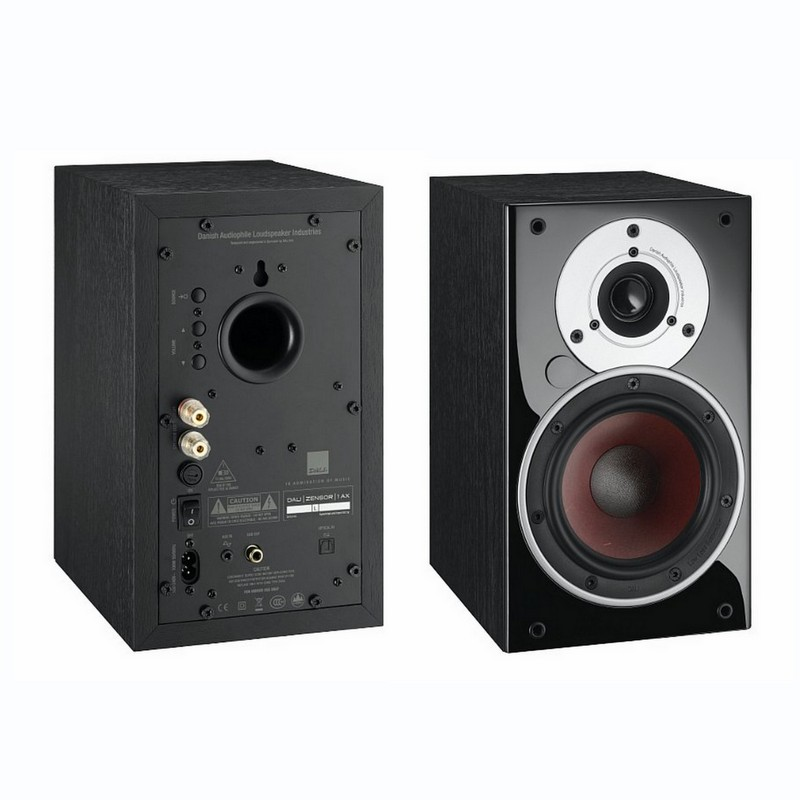
\includegraphics[width=0.5\textwidth]{figures/dali_zensor_1_ax.jpg}
% \caption{The system will be developed upon the DALI Zensor 1 AX.}
% \label{fig:dali_zensor}
% \end{figure}

% In the following sections, there will be an analysis on how the sound can be improved.

% \todo[inline]{Ikke gennemlæst}






